\documentclass[a4paper]{report}
\usepackage[T1]{fontenc}
\usepackage[utf8]{inputenc}
\usepackage{amsmath}
\usepackage{geometry}
\geometry{verbose,tmargin=1.5in,bmargin=1.5in,lmargin=1in,rmargin=1in,headheight=1in,headsep=1in,footskip=1in}
\usepackage{float}
\usepackage{calc}
\usepackage{graphicx}
\usepackage{setspace}
\usepackage{esint}
\usepackage{xcolor}
\usepackage{hyperref}
\usepackage{url}
\usepackage{soul}
\usepackage[round]{natbib} 
\makeatletter
\@ifundefined{showcaptionsetup}{}{%
 \PassOptionsToPackage{caption=false}{subfig}}
\usepackage{subfig}
\makeatother
\usepackage{float}
\raggedbottom
\doublespacing
\usepackage[showframe]{geometry}
		\usepackage{array, caption, tabularx,  ragged2e,  booktabs}
		
\let\oldthispagestyle=\thispagestyle % If we want to see a page number.
\def\thispagestyle#1{} % If we want to see a page number.
\let\oldsetcounter=\setcounter
\def\setcounter#1#2{}

% this code block defines the new and custom floatbox float environment
\floatstyle{ruled}
\newfloat{floatbox1}{t}{lob}
\floatname{floatbox1}{Box}
\newenvironment{floatbox}{\begin{floatbox1}\sf\small}{\end{floatbox1}}


% Please do not delete
\newcommand{\agr}[1]{\noindent{\color{red}({\small \sf #1})}} % axel's
\newcommand{\oga}[1]{\noindent{\color{blue}{\small \sf #1}}} % orestes'
% Orestes, please make your own comment command if desired.

\DeclareMathOperator{\cov}{cov}
\DeclareMathOperator{\var}{var}
\DeclareMathOperator{\log}{log}
\DeclareMathOperator{\min}{min}
\DeclareMathOperator{\max}{max}
\DeclareMathOperator{\det}{det} 
\DeclareMathOperator{\d}{d} 
\usepackage{babel}

\begin{document}

\pagenumbering{arabic}

% titlepage stuff
\title{Evolutionary mechanisms constraining attack rates}
\author{Orestes Uxio Gutierrez Al-Khudhairy \\
\\
Submitted in partial fulfillment of the \\
requirements of the Degree of Doctor of Philosophy\\
\\
School of Biological and Chemical Sciences\\
Queen Mary University of London
}

\date{2020}

\setcounter{page}{1}
\maketitle

\newpage

I, Orestes Uxio Gutierrez Al-Khudhairy, confirm that the research included within this thesis is my own work or that where it has been carried out in collaboration with, or 
supported by others, that this is duly acknowledged below and my contribution indicated. Previously published material is also 
acknowledged below. I attest that I have exercised reasonable care to ensure that t
he work is original, and does not to the best 
of my knowledge break any UK law, infringe any third party’s copyright or other Intellectual Property Right, or contain any confidential material. I accept that the College has the 
right to use plagiarism detection software to 
check the electronic version of the thesis. 
I confirm that this thesis has not been previously submitted for the award of a 
degree by this or any other university. 
The copyright of this thesis rests with the 
author and no quotation from it or 
information derived from it may be published without the prior written consent 
of the author. \\

Signature: \\

Date: 28/09/2020

Details of collaboration and publications: Not Applicable


\newpage

\abstract{According to adaptationism, alleles conferring higher immediate relative fitness are expected to drive the substitution of traits in species' populations. If higher hunting/foraging intensity (henceforth referred to as attack rate) offers a selective advantage to predator/consumer individuals, adaptationism implies that attack rates should always evolve to increase within their populations. Problematically, resource populations will go extinct after threshold levels of attack rates are reached. This continuous increase in attack rates, driven by natural selection and expected by adaptionism, paradoxically implies that consumer populations should evolve to overexploit all their resources in the absence of any evolutionary constraint. This contrasts with  empirical studies that show animal populations are sustained but do not overexploit their resources, such that they lie in the limited range that yield feasible food-webs. This thesis is inspired by the paradox implied by adaptationism, and aims to provide a general mechanistic explanation for how consumers avoid the overexploitation of all their resources. The framework I used to address this problem has two parts. The first is a dynamical, food-web assembly system, in which the evolution of attack rates is simulated without any explicit constraints. In this first part I derive and explain how the "live-fast die-young" trade-off, between invasive ability and local patch persistence, emerges from the underling simulation and constrains attack rates. The second part of the framework uses a patch-specific simplification of a metacommunity to test the robustness of the live-fast die-young trade-off against instraspecific evolutionary forces.}



\tableofcontents

\newpage

This thesis was completed with ample support from a network of colleagues, friends and family. I would like to firstly express my sincere gratitude to Dr. Axel Rossberg for his persistent effort that guided my research at Queen Mary from the day I enrolled. His patience, motivation, and knowledge have indescribably helped my research and writing of this thesis. His energy and enthusiasm propelled us both through every hurdle encountered along the way. I would also like to thank the rest of my thesis committee: Dr. Pavel Kratina and Prof. Andrew Leitch for their encouragement, insightful comments and constructive criticism that inspired me to broaden my research goals and perspectives. \\
 

 I thank my fellow PhD and Masters students with whom I have enjoyed priceless camaraderie, stimulating discussions and many hilarious moments. Much appreciation is also owed to Phil for organising social events that would distract us from our dedicated work ethic and bring us all together.\\

Last but no least, I would like to thank my family. My sister in particular for showing me the beauty and joy of immersing oneself in the study of biology, and my parents for all the confidence and support they have given to me.\\

This research was supported by the fully funded studentship offered by the School of Biological and Chemical Sciences at Queen Mary University of London.

\newpage

\section*{Summary}

In this thesis will firstly argue that the explanations for how attack rate are constrained have yet to be formally tested and mechanistically compared. The first chapter of this thesis aims to address this by not only formally introducing the nature and history of the problem, but also explicitly comparing key theories and ideas which have been conceived to understand it (or have a potential for doing so). The culmination of this chapter is the proposal of a two-part mathematical framework for analysing which of the reviewed constraints are most significant. This framework guides the subsequent method driven chapters. Analysis of this framework allows me to mechanistically uncover a novel negative ecological feedback that emerges from the co-evolution of consumers and their resources. \\

 My main finding and original contribution to this area of research is the derivation of the live-fast die-young trade-off, which I propose as being a universal evolutionary constraint on attack rates. In particular, I find that stronger attack rates of consumer species are more likely to cause the local extinction of their important resources via a process called serial extinction\footnote{The iterative loss of a consumer's resources driven by resource mediated competition}. Consumer species with initially higher attack rates at the point of invasion are subsequently rendered the most vulnerable to extinction by exploitative competition. In this scenario a trade-off subsequently presents itself: The initial invasive fitness advantage associated with higher attack rates is mitigated by the higher probability of local extinction. Maximising long-term fitness with respect to the live-fast die-young trade-off, subsequently yields intermediate attack rates as being the fittest in the long term. \\
 
The second original contribution of this thesis is the framework used to derive and test the live-fast die-young trade-off. This is formally explained in the second chapter, where I highlight a crucial problem that underlies mathematical models frequently used in theoretical ecology and adaptive dynamics. Specifically, the intractability of finding equilibrium solutions of complex non-linear dynamical systems, which hinders the understanding of what types of species are most likely to go extinct. The second objective of this chapter is therefore to introduce a novel mathematical framework that approximates these equilibrium solutions, in such a way that they become tractable. In so doing I am able to elucidate ecological and evolutionary activity that would otherwise remain hidden, and which are crucial for answering the question of this thesis. The third chapter simulates and analyses this approximation of the full model and culminates in the definition of the live-fast die-young trade-off.\\

 The second part of the framework is finally tackled in the fourth chapter, which is dedicated to testing the robustness of the live-fast die-young trade-off relative to the problem of cheaters\footnote{A term used in evolutionary game theory, usually in problems related to the tragedy of commons. Cheaters denote individuals that adopt strategies for using a limited common resources that only benefit their own individual fitness. Furthermore, if all individuals adopt the cheating strategy, the common good will be exhausted and render the competing population extinct.}. The final chapter serves as a platform for comparing the ecological signatures expected by the live-fast die-young trade-off to field observations. Given the ultimate mechanism for enabling the trade-off is rooted in overexploitative behavior, I focus on studies of species invasions that exhibit so called "boom-bust" dynamics\footnote{A phenomenon found in the studies of invasive species. These dynamics denote a mysterious disappearance (the so called "bust") of an invasive species that had initially grown to significant population sizes (the "boom").}. The chapters in this thesis therefore represent four distinct and necessary stages for understanding how attack rates are evolutionarily constrained in complex bi-partite food-webs composed of consumers and resources. \\
 
 
The programming code used to create the simulations, analysis and documents relating to this thesis can be found in the following repository: https://github.com/OreUxio/Ecological_Mechanisms_Constraining_Attack_Rates



\chapter{Types of constraints on attack rates \label{ch:chapter_1}}

In this chapter I will address the question of whether attack rates can be argued as being constrained. A subsequent evaluation on the ability of different kinds of potential evolutionary constraints is provided. To conclude, I present a modeling framework for understanding which is the most active mechanism in constraining attack rates. This framework forms the basis of the ensuing method driven chapters. The following s will firstly highlight the paradox at the heart of this thesis: The naive expectation for natural selection to continuously increase attack rates and thus annihilate resources. This contrasts the apparent balance observed between predator and prey in nature. \\

\section{Evolutionary suicide induced by resource overexploitation}

The idea that species may evolve to limit and even damage their survival, such that this may lead to their extinction,  was first introduced by \citep{Haldane1932} with reference to cases from the fossil records where ‘‘… species literally sank under the weight of their own armaments’’. This phenomenon, referred to as as “Evolutionary Suicide” by \citep{Parvinen2005} and “Darwinian Extinction” by \citep{Webb2003} has been further documented empirically in a variety of biological systems, as reviewed by \citep{Rankin2005}. In terms of attack rates this was first discussed empirically in the two-species predator-prey mite experiments by \citep{gausse1934} and \citep{Gause1936}. The conclusion of these experiments is that predatory mites are doomed to annihilate their prey unless the latter have areas of refuge from predators from which they may repopulate overexploited areas. Formal mathematical treatments of evolutionary suicide that since arose in the field of adaptive dynamics have been reviewed by \citep{Ferr2004}, who found evidence contrary to the expectation that natural selection should always maximise fitness. Indeed, the authors argue that maximisation of fitness is the exception rather than the rule, such that most common expectation is for evolutionary suicide to occur. \citep{Parvivnen2013} confine cases that guarantee evolutionary suicide through optimising selection to two scenarios, one of which is the tragedy of the commons\footnote{A scenario conceived by \citep{Hardin1968} originating from game theory and which and is used to describe a variety of ecological and evolutionary scenarios, as reviewed in \citep{Rankin2007}. In biology, the tragedy of the commons concerns the strategic choices that individuals/species make when competing for are shared limited resource. If they all cooperate to share the resources fairly, everyone wins (i.e. all competing agents are able to persist), if they all attempt to outcompete each other, they will overexploit the resource and loose}. Thus it is a problem of particular interest to this thesis. The cooperative case requires foresight however, which lead \citep{Parvivnen2013} to raise the question of “ .. why does life generally persist?” if selection does not operate with foresight and pushes individuals toward ever higher harvesting intensity and growth rates in a world of limited resources. \citep{Parvivnen2013} argue that there are two possibilities resulting from the conundrum of evolutionary suicide. Either the resulting extinctions are indeed widespread (given the relatively frequent extinctions reported in the fossil record) or there are mechanisms that can potentially prevent evolutionary suicide. The authors list these mechanisms as ranging from cost-benefit trade-offs associated with traits, emergent constraint from co-evolution of species, or spatial structures and relatedness of individuals that allow cooperative strategies to be selected for. Similar mechanisms are discussed in a review by \citep{Rankin2007} for mitigating the tragedy of the commons. In this chapter, I will argue that the question still remains formally unanswered for general consumer-resource models. \\

The problem of overexploitation can be explained mathematically using a simple simulation in adaptive dynamics, similar to the examples treated by \citep{Johansson2013}, used to represent the problem of overexploitation mentioned earlier. The evolution of a consumer (C) that relies on a finite resource (R), with consumer-resource dynamics of the form:

\begin{sub-equations}
  \label{eq:LV11}
  \begin{align}
    \frac{dR}{dt}=\Biggm[ s \Biggm( 1-\frac{R}{K} \Biggm)-F(a_r)C \Biggm] R
\label{eq:LV_consumer11},\\
    \frac{dC}{dt}=\Biggm[ \epsilon+ F(a_r)R-\rho \Biggm] C,\label{eq:LV_resource11}
  \end{align}
\end{sub-equations}

In this system \\

\begin{enumerate}

\item Population growth and maintenance of consumers is achieved by foraging/predating the regenerative basal resource population $R$ (such as a plant), that is limited (i.e. with carrying capacity $K$) and not undergoing selection.

\item Foraging/predation occurs via the functional response $F(a_r)$ which is a function of the consumers' attack rate $a_r$ and the biomass of both resource and consumer.

\item The rate $\rho$ of biomass loss due to respiration and/or natural death of the consumer is independent of $a_r$.

\item The trait $a_r$ in the population is monomorphic, however, mutant types $a_m$ can arise randomly due to mutations.

\end{enumerate}

In this scenario, the resident herbivore population will be replaced by a mutant population if $F(a_m) > F(a_r)$ and the old residents types will go completely extinct. This iterative substitution of attack rates will continue until the foraging intensity is so high that it extinguishes the resource population. This sequence of events is an example of the evolutionary suicide that is expected by \citep{Ferr2004} to occur generally across ecological settings.  \\

\section{Are attack rates constrained? \label{sec:weak}}

Consider the case $F(a_m)=a \times R$ (a type I functional response first proposed by \citep{Holling1959}), we would expect unconstrained optimising selection to continuously increase $a$, the attack rate. If we entertain the idea that evolutionary suicide induced by overexploitation is a general phenomenon, one might expect a prevalence of ever increasing attack rates $a$ driven by unconstrained trait optimisation. However, this would be at odds with the prevalence of weak or intermediate-strength trophic links (which include attack rates) reported across empirical food-webs by \citep{Paine1992} and \citep{Berlow1999}. Indeed, by parametrising attack rates according to predator-prey size ratios \citep{guzman2019}, (such that attack rates are $a = f(m_p,m_v)$, are isotropic functions of predator-prey mass ratios) shows that intermediate attack rates maximise species persistence in food-webs. Considering the possibility of non-adaptive stability selection of food-webs \citep{Borrelli2015}, one would expect configurations that allow for species persistence, such as intermediate interaction strengths, to be observed more frequently. Indeed, the quantitative analyses of \citep{guzman2019}, \citep{Brose2006a} and \citep{Pawar2019} have repeatedly shown that observed species’ attack rates remain in ranges predicted to permit persistence and coexistence within food-webs. This suggests that at a type of constraint on attack rates is active, a conclusion strengthened by evidence found in the review by \citep{Futuyma2010}, which highlights the paradox of attack rates remaining in a feasible range despite an abundance of genetic variation. The implication is that large amounts of genetic variation should in principle lead to instances of rapid local adaptation. Instead, according to a review by \citep{Pearson2001}, evolutionary stasis (which is an evolutionary failure to adapt) is found to be the norm. Specifically the authors point to the meta-analysis of fossil records published between 1972 and 1995 by \citep{Pearson2001} which found that 71$\%$ of species exhibited stasis. Other species cases are also reviewed, for example, in \citep{Choen83} species of gastropods and bivalves were collected and shell morphologies measured (dating from within the time period of 1.3 to 4.5 million years ago). Although three instances of rapid evolutionary change of shell morphologies occurred, these were the result of ecophenotypic\footnote{Plastic phenotypic variation between populations that are due to respective environmental differences and responses} responses to environmental perturbation, such that once the environment returned to normality, so did shell morphologies. Their final analysis, based on multivariate analyses of lineages, showed little variation from the mean within each lineage, and thus demonstrated the ubiquity of stasis.\\

Evolutionary constraints may appear via a variety of mechanisms that are not explicitly controlled for in Gausse's doomed mites experiment and the simulations underlying Eq. \eqref{eq:LV11}. These are over-simplification of reality that do not account for the arising complexities of species evolving in ecosystems. Some have proposed that constraints on attack rates may emerge from the co-evolution of predator and prey, rather than being defined a priori, as in the life-dinner principle \citep{arms_race}. This principle assumes that natural selection acts more strongly on prey than on predators, because the former fight for their lives rather than their dinner. Every increase in a predator’s ability to forage and hunt for resources is subsequently met by an equal if not larger increase in the prey’s ability to evade. More complications occur when considering other dimensions of fitness that underlie the evolutionary trajectories of attack rates. Firstly, allopatric populations facing different environmental conditions do not evolve as they would in isolation. \citep{Thomas2002} for example review how gene flow between allopatric populations can counteract the effects of natural selection so much so that they may undergo gene swamping\footnote{When an allele has an environmentally associated advantage over others in a specific geographic location, but it is lost because the rate of dispersal of other alleles from a much larger nearby population is overwhelming}. Secondly, there is a temporal dimension to fitness (reviewed by \citep{Hendry2018}) that manifests itself via the interaction of traits and the surrounding environment, which may change due to inherent stochasticity or environmental (see \citep{Brisson2018}) and social feedbacks (see \citep{Nowak2012}). Thus fitness is defined as a geometric average of lifetime reproductive output through time (assuming the special case of fixed generation times). The spatio-temporal dimensions of fitness are illustrated in a theoretical review on the evolution of virulence in pathogen-host metacommunities \citep{Goodnight2008}, which discuss how a trade-off between invasiveness fitness and persistence allows types of intermediate virulence to be fittest, thus avoiding the decimation of hosts they rely on. The authors argue this trade-off can only be understood at the metacommunity level, by appreciating the feedbacks that are driven by changes caused to the environment such that “… descendants may have different reproductive success than their ancestors of the same genotype”. Their reasoning led to the hypothesis that there is a trade-off between invasion fitness and persistence, that rewards “prudent” predators, i.e. those with intermediate attack rates, making them the fittest. \\

 The resurrection of prudent predation is potentially polarising in evolutionary theory however. Prudent predators were first envisioned by \citep{Slobodkin1968}, who argued that the feedback produced by predator-prey co-evolution constrains predators to adopt strategies that promote the survival of the resource they rely on. Slobodkin originally posed that by feeding on life-stages that minimise the impact on the resource's fitness, i.e. those with the lowest reproductive value, predators are able to maximise the lifetime and sustainable use of a resource source (the prey). Such an environmentally induced feedback implies that species evolve to exist within the limits permitted by their surrounding environment, implying that the conclusions from experiments like \citep{gausse1934} and \citep{Gause1936} cannot be extrapolated, because they do not account for the joint natural conditions of predator, prey and surrounding environment. Indeed, \citep{Goodnight2008} advocates the importance of integrating the ecological effects of different interacting populations, i.e. the meta-community, and associated feedback experienced by species. This resonates with a review by \citep{Leibold2004} that emphasizes how insights driven by a meta-community analysis may contrast with those obtained from local communities. As argued by \citep{Goodnight2008}, pathogen-host metacommunity systems can be considered similar to that of predator and prey in that they both resemble the tragedy of the commons: both predators and pathogens compete inter and intraspecifically over a respective limited prey and hosts, the resource. The maximisation of intra and interspecific competitiveness then results in the exhaustion of that resource. Although the ultimate mechanisms enabling the trade-off for realising “prudent” pathogens may be analogous to one enabling “prudent” predators, it is not directly translatable at face value: The vast majority of parasites and pathogens have life cycles and hence, rates of evolution that are much faster than their hosts for example, which makes it easier to evolutionarily adapt to specific hosts and host availability. Furthermore, the negative feedback enabling the trade-off depends on the death of hosts, which in terms of units of biological organisation that compose them, are many orders of magnitude of larger than that of pathogens. Thus the question of whether a similar trade-off is operating in predator-prey metacommunities, such that it renders intermediate attack rates as the fittest strategies, remains open.\\

At this point I argue that there is evidence for the existence of some mechanism to constrain attack rates to remain within the feasible range, such that predator and prey may persist, i.e. within “prudent” levels. The mechanisms proposed to generate seemingly prudent attack rates are far and wide however. The objective of this chapter is to quantitatively analyse the ability of each mechanism to mitigate evolutionary suicide induced by overexploitation. I will therefore evaluate theories aimed at explaining how species traits are constrained, and, which originate from a variety of sub-disciplines in biology (namely population and quantitative genetics, evolutionary game theory and adaptive dynamics). I will discuss the evidence that has been brought forward to promote or revoke them. Using the following criteria, I will evaluate whether they are viable explanations with wide-ranging applicability across biota:  

\begin{itemize}
\item Their ability to allow for the feasible co-existence during the co-evolution of consumers and resources despite natural selection.
\item The complexity of mechanism and their resulting ease of applying generally across lifeforms that depend on limited biotic resources. 
\end{itemize}

I will argue that many of these mechanisms are incapable of fully explaining how attack rates are universally (i.e. across all taxa) evolutionarily constrained and thus, the problem of overexploitation is not fully resolved. Indeed, they are either i) at best contextual and applicable to certain scenarios only, ii) subject to evolutionary forces themselves and can therefore be selected for or against (implying that these immediate constraints might be the result of higher-level evolutionary constraints), iii) dependent on the specific interaction of the evolutionary history of a species lineage and the environment (i.e. they occur by chance and cannot be relied upon) iv) or are yet to be formally tested and proven.\\

The final product of this chapter is a modelling framework for subsequent quantitative analysis, which combines the most plausible and relevant mechanisms. Specifically, I will seek to build a minimal model that achieves feasible and realistic food-webs. This model will allow these mechanisms to be isolated, and their phenomenological signature determined, thus permitting in-vivo/vitro testing of any hypothesised mechanisms. The framework should not depend on a specific mechanism applicable only to a subset of species, and instead should focus on those mechanisms that are shared by most (if not all) systems of consumers that rely on limited resources (in particular grazers-plants and predator-prey systems). \\

\section{Potential mechanisms for constraining attack rates}

\subsection{Foraging behaviour, prey density and prey switching \label{sec:forage}} In a model that uses Brownian motion to simulate the dynamics of a predator searching/foraging for prey located in a two dimensional system, \citep{Basset1997} show that the subsequent low density of the resource induced by the foraging efforts of the predator, translates into low prey encounter rates that stall consumer population growth. As a result, prey overexploitation becomes more difficult. \citep{Humphries2010} however show that when prey is scarce, consumers may switch from this type of search pattern to the more efficient Lévy flight foraging behaviour, that increases encounter rate even when resource are scarce. This suggests that for prey to rely on low density as a defence mechanism is not feasible, given that even predator behavioural plasticity can circumvent this. As discussed as early as \citep{Holling1961} and more recently empirically argued by \citep{Jaworski2013}, in a more complex community with many resources, predator’s switching between prey may occur, such that the consumer can rely on other resource populations when one is too low. This is used by \citep{Murdoch1975} to explain how resource overexploitation may be mitigated: Prey-switching between two resources by foraging more intensely on the most abundant, allowing the other species to recover, generates synchronized cyclical dynamics between the two resources. However the general behaviour of the simulation of a consumer foraging on two resource species by \citep{Tanksy1978}, is for the system to stabilise rather than generate the cyclical dynamics expected to alleviate foraging pressure on scarce prey. Furthermore, \citep{Abrams2003} compared a variety of prey-switching type models that incorporate the effect of low prey density simply found an increased likelihood of exclusion of the slower growing prey. Finally, in the empirical review of \citep{MAtter2005} cases are documented in which prey switching could have occurred, but did not, and argue that for prey to rely on scarcity to survive implies chance (i.e. if the traits of predator and prey would have evolved slightly differently, persistence of prey would not have occurred). In conclusion, there appears to be no need to include a complex functional responses to simulate prey switching in Eq. \eqref{eq:LV11} in the hopes of it constraining attack rates. \\

\subsection{Predator-prey arms race \label{sec:arms_race}} Describing attack rates as a function $a(f_r,v_r)$ of consumer foraging ability, $f_r$, and resource vulnerability, $v_r$, provides the setup for an evolutionary arms race (for further details see \citep{rossberg09:_how_troph_inter_stren_depen_trait}). As discussed earlier, the life-dinner principle conceived by \citep{arms_race} assumes that selection acts more strongly on prey than on predators. If the predator fails to capture its prey, it can try again, whereas if the prey fails it will be removed from the gene pool. The prey’s vulnerability traits should therefore evolve faster than the predator’s foraging traits, in such a way that predators will not be able to over-exploit their prey. \citep{Abrams1986} analysed different models of predator-prey co-evolution (under the conditions that adaptation of one trait comes at the cost to another). They questioned the applicability of the life-dinner principle by showing that the direction of selection of a predator’s trait depends on the shape of a cost-benefit function and the population dynamics of the predator-prey system. Furthermore, the authors find cases of asymmetric trait evolution of predator and their respective prey in the fossil record. Predator morphology did not change in response to apparent changes of prey morphology thought to have decreased its susceptibility to predation. Moreover, the authors point out that increasing the complexity of food-webs disrupts the effects of fitness changes on foraging and defensive ability: A change in defensive trait that may protect from one predator species, might make it more vulnerable to another, reducing the potential increase in fitness. Whereas for the predator, a change in foraging traits directed at increasing attacks rates on one species may disrupt potential attack rates on other resources. Finally,  detailed studies of food-web topologies, either on their
own \citep{rossberg05:_props_with_corr} or in comparison with
phylogenetic data
\citep{bersier07:_signat_of_phylog_const_food_web_struc,
  Eklof16:_PhylogeneticComponent}, consistently show that in a joint
niche space in which the predator traits need to match prey traits to
attain a maximum attack rate
\citep{rossberg09:_how_troph_inter_stren_depen_trait}, prey tend to
evolve much slower than predators.\\

It has also been found that the arms-race scenarios (i.e. between competitors and/or predator and prey) may not act to stabilise food-webs, as expected by the life-dinner principle, and may instead lead to extinctions driven either by “escalation” or “co-evolution”, as discussed in the empirical and theoretically reviews by \citep{Dietl2002} and \citep{Vermeij2013}. The process of “escalation” describes an enemy driven evolutionary arms-race, whereas “co-evolution” is that driven by predator and prey. \citep{Vermeij2013} describes escalation as a species’ trait adaptations that are driven by species competition (that are energetically costly) rather than environmental niches (such as geological and climatic factors). He argues that species require more resources to survive relative to when they forage with no other competitors, since they must fuel the traits that allow them to compete. The trade-off for this behaviour occurs when the resources that species depend decline in abundance, via environmental perturbations for example. Given the consumers cannot suddenly shed the energetically costly traits required for competition, they are now more vulnerable to extinction. Evolutionary suicide driven by predator-prey arms-race can also be of the type theoretically studied by \citep{Matsuda1994}, where prey extinction (and subsequently that of the predators) occurs if there is a trade-off between the prey’s intrinsic growth and anti-predator defence. In these simulations predator defence is selected for at the cost of population growth in the prey, thus as foraging efficiency increases via selection, the prey will ultimately starve. Therefore, the inclusion of foraging and vulnerability traits may simply exacerbate extinctions, driven by escalation and co-evolution, rather mitigate them. I will therefore not include them to minimise complexity and simplify subsequent analysis.\\

\subsection{Genetic trade-offs resulting from pleiotropy and epistasis \label{sec:genetic_tradeoffs}} Genetic trade-offs due to pleiotropy and epistasis are a type of biological constraint that results from biotic properties. Specifically, pleiotropic constraints highlight an incompatibility of traits whose joint realization are not practically possible due to the history of selection that has acted on the genetic structure of a species. These genetic effects are usually studied via negative correlations between the phenotypeic traits they define, and are widely reported as extensively reviewed by \citep{Walsh2009} and \citep{Hughes2018}. Furthermore, according to \citep{Hillerislambers2003} negative correlations between traits can increase species coexistence in food-webs by mitigating the ability of evolution to strengthen destabilising species interactions. A clear example of this is given by \citep{Rainey1998}, whose evolutionary experiments on populations of \textit{Pseudomonas fluorescen} revealed how the advent of diversification within identical population depended on the heterogeneity of the environment. The authors subsequently propose that evolutionary trade-offs in competitive ability drive adaptive radiation, given that biodiversity tended toward heterogeneity / homogeneity depending on whether the environment populations was heterogeneous / homogeneous. The reasoning being that, had trade-offs not significantly affected evolution, biodiversity would have been homogeneous even in the heterogeneous landscape. Concrete empirical examples of pleiotropy limiting the evolution of traits are reviewed by \citep{hoffmann2014evolutionary} and include the trade-off present in \textit{Eschera coli}: Their ability to adapt to low temperatures comes with the cost of reduced ability to evolve in environments with fluctuating temperatures. Another example is that of the \textit{Lythrum salicaria} wetland plant. The invasion of \textit{Lythrum salicaria} into relatively colder latitudes was possible via an adaptation that allowed it to flower early. However, this came at the cost of a smaller flower size compared with individuals from warmer areas.\\

 A constraint on attack rates due to pleiotropy could arise in the following way: If the fitness increase from a mutation associated with trait \textit{A} underlying attack rates, is met by a simultaneous fitness decrease caused by the pleiotropic effect that the initially beneficial mutation has on another other trait \textit{B} (or set of traits). New mutants attempting to establish with larger attack rates would then have no fitness advantage over the residents, resulting in an evolutionary stable strategy ESS \footnote{One that renders a species immune to invasion from any other mutant type of that same species in the same environment}. However, this explanation firstly implies that the constraint occurs by chance, given that an ESS would have to occur precisely in the range that ensures feasibility. Secondly, according to the review by \citep{Cheverud2015}, the structural topology of genetic interactions at different loci (which are modelled using gene interaction matrices), tell us that pleiotropic effects are shaped by the preceding history of selection acting on the underlying interacting loci. This means that trait correlations derived from pleiotropic trade-offs cannot be considered to be fixed if the underlying genetic machinery that controls them can be selected for. As a simple example (discussed by \citep{Cheverud2015}), is that of selection acting on two interacting loci which increases positive correlations between the respective traits, whereas selection acting only on one decreases it. One of the most famous examples of positive trait correlation is the landmark study by \citep{Lande1979} for example, which studied the relationship between body-size and brain-size. It can be argued therefore that the ultimate cause for negative correlations between traits is the process of selection that has shaped the lineage for many generations. The pleiotropic effects observed on the other hand, are the proximate causes of trait correlations and trade-offs. Thus including trade-offs associated with pleiotropy in a simulation, requires models using gene interaction matrices (reviewed in \citep{Cheverud2015}), or at the very least, a simplification of this that accounts for the effect of selection. Evidence that trade-offs can be selected for can be found in experimental study of the evolution of phage resistance of textit{Escherichia coli} cells by \citep{Burmeister2020}. The authors discuss how phage selection can either result in bacteria showing increased antibiotic sensitivity (a negative trade-off) or not, depending on the mutations present. Given that selection may simply act to decrease the strength of trade-offs and be selected for, including pleiotropic effects are unlikely to aid the identification of constraints on attack rates.\\

\subsection{Physiological constraints \label{sec:physiological_constraints}} Physiological constraints are another type of biological constraint. They denote an impossibility of certain trait combinations given the restraint imposed by physical laws underlying the chemical reactions and other abiotic processes that biological activity depend on. These include those underlying metabolism and several others \citep{Pauly2017},\citep{Brett2000}. I focus on metabolic constraints as described by the metabolic theory of ecology (originally proposed by \citep{brown}, \citep{Savage2004}) because these are thought to be universal to all living organisms, making them plausible universal constraints on attack rates. MTE states that the physical laws governing (and constraining) chemical reactions for the growth and maintenance of cells, scale up to the growth of and maintenance of individuals, and therefore to entire populations \citep{brown}. A constraint on predator population growth, if calibrated accordingly relative to that of the prey, might thus mitigate the problem of overexploitation. From a modelling perspective, correlations between between traits can be included via their respective allometric scaling with body mass as reviewed by \citep{Pierre2019}, where the authors discuss how these correlations can promote food-web stability. They are also powerful predictive tools, \citep{Pawar2019} for example predicted which predator-prey body mass ratios permit feasible coexistence in nine empirical communities, both terrestrial and aquatic. They achieved this firstly by comparing theoretical predictions of feasible pairings to empirically existing ones, and by simplifying typical food-web dynamics to a) consumers being able to overcome respiration, and b) predator-prey co-existence based on simple two-species consumer-resource equilibrium solutions. It is not clear however how these body-mass ratios remain in the predicted stable range however. I argue that to rely on metabolic constraints on traits as a universal constraint on attack rates that mitigates overexploitation in predator-prey systems again implies chance. This is because the trait correlations within predators would have to be calibrated according to those of their prey. Furthermore the chances of this occurring decreases if we acknowledge that these correlations vary according to genetic backgrounds. As shown by \citep{Werner2018} for example, endotherms require more energy to maintain a certain body temperature than ectotherms. Finally, the actual scaling relations are not as simple as often assumed. For example, \citep{Pawar2012c} show how differences in metabolic scaling occur depending on the dimensionality of the medium (land, water or air) species live in. \\

\subsection{Dispersal between patches and the “rescue effect” \label{sec:Dispersal}} The experiments by \citep{gausse1934} and \citep{Gause1936} on prey annihilation, with two species of mites (one predating on the other), lead to the conclusion that an area of predator refuge is required to rescue the prey in overexploited patches to avoid their global annihilation by predators.\citep{HuffakerC.} reasoned that local extinction of prey does not imply total extinction however. Instead, sources of immigration required to mitigate overexploitation need not necessarily be areas of refuge that are completely inaccessible to the predator, but rather other patches not yet overexploited by them. The associated effect of disparate patches acting as sources of refuge and propagule generation is nowadays referred to as the “rescue effect” \citep{Utherland2012}. \citep{HuffakerC.} thus extended Gausse's predator-prey mite experiments using multiple patches. The hypothesis to test was whether increasing the complexity of the patch network could guarantee the survival of the prey, given the subsequent disruption of dispersal rates. However, their setup only delayed the inevitable annihilation of the prey. Given that increasing patch connectedness significantly increased survival time, the authors concluded that in a more tailored experimental setup, long-term coexistence might be achieved. These experiments generated much curiosity about the effects that varying types and degrees of connectedness within the natural world have on species interactions, as reviewed by \citep{Levin1976}. The authors concluded that the heterogeneity of the environment (either externally imposed or emerging from random events magnified by species interactions) and the potential for dispersal of species, may lead to a system that is at equilibrium at the metacommunity level, even though the individual constituent connected sub-systems are not. This mechanism thus permits the existence of species that are locally overexploitative, via the use of spatio-temporal strategies involving local fluctuations, such that they capitalise on resources that “although locally ephemeral, may be globally very dependable”. It is clear however, that this persistence requires the rate of dispersal of both predator and prey to be in a specific range to avoid starvation of the predator (i.e. when predator/prey dispersal is too low/high) and annihilation of the prey (i.e. when predator/prey dispersal is too high/low). This is highlighted in the numerical simulations by \citep{Hilborn1975} that were inspired by the mite experiments of \citep{HuffakerC.} and \citep{Hastings1977}. The simulations show how although increasing the number of connected patches always increased the chances of persistence, the effect of decreasing/increasing predator/prey dispersal ability is non-linear: at first this increases the chances of persistence, but after a certain threshold the effect is reversed. If selecting for the dispersal rates of predators has the same effect as selecting for attack rates, in that their unconstrained evolution will lead to overexploitation and annihilation of their resources, there must also be constraints acting on the dispersal rates of consumers to achieve stable coexistence with their biotic resources. Thus it would seem that including dispersal only adds to the problem, since we now face two biotic parameters (attack rates and dispersal) that can potentially evolve in such a way as to annihilate the resource.\\

Interestingly, a trade-off between dispersal and competition ability - first envisioned by \citep{levins1971} and extensively reported in nature \citep{yawata2014} and \citep{William2006} - is known to facilitate coexistence of species in a multi-patch system that would otherwise lead to dominance of one in a single patch (i.e the better competitor). If we consider increasing attack rates as implicitly increasing a species’ competitive ability, then this trade-off could also potentially be acting on dispersal and attack rates. In a simulation by \citep{Pillai2012}, where species evolve according to a trade-off between dispersal and interspecific competition rates, it is found that co-existence of many competing species is indeed theoretically possible. This is subject to the condition that local extinctions driven by competition are stochastic rather than deterministic. Species thus initially evolve to decrease their dispersal ability and increase their competitiveness instead. This continues until a steady-state is reached, such that dispersal abilities never decrease past a critical value, relative to the patch-wise natural death rate, that would lead to extinction. This equilibrium implies that a constraint on the evolution of interspecific competition is possible if there is a dispersal trade-off associated with it. This further implies that a constraint on attack rates might also be possible given the association of interspecific competition and attack rates. Problematically even if the exact nature of the underlying mechanisms of the trade-off between dispersal and competitive rates were known and included in a study similar to \citep{Pillai2012}, such that a competition-dispersal steady-state is reached, it is unclear whether this would mitigate overexploitation. This is because the explicit dynamics of resources and consumers, and indeed the biomasses for which a steady-state is reached, are not explicitly considered. Therefore, we may not judge the feasibility and realism (such as non-negative biomasses) of any steady-state that is reached.\\

A similar stabilising trade-off is studied by \citep{Goodnight2008}. Specifically, \citep{Goodnight2008} discuss how a trade-off emerges in co-evolution of parasite-host metacommunities between invasive ability - analogous/correlated to dispersal ability - and persistence - comparable to the competitive ability studied in \citep{Pillai2012} - which renders intermediate types of virulence fittest. This fitness trade-off is then argued to potentially be occurring analogously in predator-prey meta-communities: Overexploitative behaviour initially grants increased likelihood of patch invasions (i.e. higher dispersal rates) at the cost of weakening the local environment in such a way that it reduces the resident’s ability to locally persist. \citep{Goodnight2008} thus argue that we must view fitness as changing with time, given the feedback created by the interaction of traits and environment: strains/mutants deemed to be immediately fitter, i.e. in the short-run, may over-exploit the underlying environment so much that lifetime fecundity is no longer an efficient measure of long-term success. It implies that we must be conscious of the reality of descendants' having different reproductive success relative to their ancestors (even if they have identical genotypes). Therefore the spatial treatment of this scenario is argued to be critical to permit the time-dependent distinction of the ability to invade and the ability to persist. Furthermore this spatial treatment should not be averaged as usually done in gene-centric studies and mean-field treatments. A mechanistic understanding of how the trade-off reported by \citep{Goodnight2008} may occur more generally in predator-prey food-webs is still required however.\\

\subsection{Complex food-webs \label{sec:complex_foodwebs} }

There is evidence to suggest that identification of the fitness trade-off required by \citep{Goodnight2008} can be studied in assembly models that approximate meta-community type dynamics. The community consumer-resource assembly model by \citep{Pawar2009} adds consumer and resource species by sampling biotic parameters (including attack rates) from a fixed distribution, thus simplifying a multi-patch environment. The invasion-instability trade-off that emerges is argued to constrain attack rates: Species with lower attack rates, although likelier to invade, are simultaneously likelier to generate population crashes by increasing the weighted generality\footnote{A stability measure correlated with the real part of the largest eigenvalue of the interaction matrix's Jacobian. If this eigenvalue increase above zero, the system becomes unstable such that species will go extinct. Therefore, as the weighted generality increase, the food-web system is likelier to become unstable and loose species}. The nature of the instability (i.e. which exact types of species will go extinct) is not discussed due to the intractability of the system. However, given the trade-off constrains the evolution of average attack rates in the simulation, it is plausible that these instabilities create a negative feedback on species types that are likelier to invade: If there was no negative feedback, average attack rates might simply continuously increase, simply because they are likelier to invade. This assembly model does not strictly simulate evolution of attack rates however, because these are sampled from a fixed distribution, rather than from remaining the residents in the community that have not gone extinct yet. \\

This feedback has to be scrutinised further therefore, in a scenario where attack rates are allowed to evolve, to make the nature of the instability ecologically and evolutionarily interpretable. This is the case for \citep{Rossberg2008}, which successfully simulates the evolution of attack rates of consumers and resources in a food-web assembly model by sampling the base attack rate\footnote{A parameter which controls the mean of a species’ attack rate in logarithmic space.} of invaders from existing residents. Different species are differentiated by their base attack rate, the mutated parameter subject to evolution. Each new invasion within the food-web is analogous to sampling a handful of individuals from the regional species pool that are attempting to invade the local food-web/patch, therefore simplifying the metacommunity by assuming the focal patch being simulated is representative of surrounding imaginary ones. Interestingly, even though no explicit constraints are imposed in the simulation, the time-series of the averaged (over all resident consumers per time-step) base attack rate reaches a plateau. This indicates the possibility of an evolutionary constraint that emerges as a negative feedback associated with base attack rates. As explained by \citep{Goodnight2008}, this is necessary for shaping the evolutionary trajectory of attack rates in predator-prey metacommuntities, such that predators with intermediate attack rates, i.e. so called “prudent predators”, are the fittest. If the constraint on attack rates in \citep{Rossberg2008} can be mechanistically understood and subsequently tested for in a metacommunity model similar to \citep{Goodnight2008}, this may provide the basis for a universal constraint acting on attack rates in predator-prey system. \\


\subsection{Altruism \label{sec:Altruism}} I next consider how mechanisms relating to the emergence of altruistic traits in species may constrain or exacerbate the evolution of attack rates. A trait is altruistic (or cooperative) if it benefits others while bearing a cost to the trait-bearing individual. In our case study, having less exploitative traits can be considered altruistic, if in so doing the individual forgoes the immediate fitness benefit of consuming more resources but also benefits its species because there are more resources to go around. As argued \citep{Slobodkin1968} if all individuals collectively exploited resources such that they minimise the chances of driving them extinct, more consumer individuals as a whole can be supported, thus maximizing their lifetime as a species. Slobodkin’s argument was based on the observation that the value of ecological efficiency computed for laboratory populations of Daphnia and \textit{Artemia nauplii} \citep{Slobodkin1964} - that were experimentally harvested so as to maximise long-term biomass yield - were numerically close to the efficiencies calculated by \citep{Lindeman1991} and others obtained from field observations \citep{Slobodkin1960}. It is difficult to envision a process that enables prudent predators however, given that selection is “blind” and does not operate according to foresight. Some kind of negative feedback suppressing more exploitative types is required. Indeed the formal theoretical study of altruism and cooperation sparked an infamous debate surrounding the theory of group selection\footnote{A theory for how natural selection may act on groups of individuals, rather than only individuals, leading to trait selection that is advantageous at the group level. See \citep{edwards1986} for a detailed explanation}. \citep{J.MaynardSmith1964} however argued that group selection was unnecessary for explaining apparently altruistic traits. Instead these were said to arise via kin selection \citep{Hamilton1964}, which considers the fact that ultimately the unit of selection that is spreading in an environment is the allele. Individuals that share a particular allele are thus identical from the perspective of the allele type. Conferring fitness benefits to many related individuals sharing the same allele, instead of only the underlying individual, is more beneficial. Secondly, group selection was criticised for being vulnerable to the problem of cheaters, described in a review by \citep{Maclean2006} as individuals that “.. selfishly use common resources to maximize their individual reproduction at the expense of the group”. Although groups containing more altruistic traits may be fitter, they are vulnerable to the invasion of individuals that do not display altruistic traits, i.e. cheaters, and are therefore fitter at the individual level. Slobodkin’s theory of prudent predation was thus heavily criticised for relying on altruism and group selection, \citep{Society2011} for example argued that predators could either avoid prey overexploitation by depending on the spatio-temporal dynamics envisioned by \citep{HuffakerC.} which I discussed previously, or because of differences in hunting ability of individuals within predator population, which depends heavily on the interaction of population structure, environment and prey. \citep{slobodkin1974} refuted the allegation that prudent predation relies on group selection, re-iterating that it could be realised in either of three ways. The first is through an arms race similar to the life-dinner principle, which as I argued above can’t be the general explanation. The second is that predators evolve to maximise the likelihood of catching prey individuals, for example by specialising on those that are most vulnerable. Predatory evolutionary adjustments that then allow so called “prime” prey individuals to be caught although possible, subsequently become inefficient and thus selectively disadvantageous given initial predator adaptations (a theory that remains to be formally tested as a possible general constraint). Thirdly, Slobodkin suggests that deviations from prudent predation do occur and make predator-prey dynamics unstable. In this scenario, individual predators and prey responsible for such instabilities would go extinct, and their genetic information removed from their respective gene pools, such that the predator and prey populations resume stable dynamics (although Slobodkin considers this highly unlikely given that it supposes drastic environmental changes or super-mutations). \\

A concrete example of prudent predation emerges from the experimental study of predator (a planktonic rotifer) and prey (a unicellular green algae) cycles is by \citep{Blasius2020}. In these experiments, populations of predators persisted independently in a homogeneous environment for roughly 300 predator generations. This was hailed by \citep{Hastings2020}\footnote{An important original contributer to the understanding of population dynamic relationships between predator-prey relationship \citep{Hastings1977}} as ground breaking given that it is one of the few / only experimental studies that shows how predator-prey cycles can persist without external stimuli (such as the artificial addition of prey species). However as Hastings himself points out “ ... mathematical theory suggests that the small amplitude cycles observed by Blasius and colleagues would occur only under very specific conditions”. Thus the natural question that again arises is: How would a predator evolve to maintain this cycle that ensures persistence? \citep{Blasius2020}, argue that juvenile maturation is the crucial factor given it sets a phase lag (measured and detected using a time-series analysis) between prey density and the ratio of egg to predator individuals. When the maturation was set to zero in a simulation that replicates the predator-prey dynamics, the lag between prey density and egg ratio disappeared. The effect of juveniles on the phase difference is crucial for realising persistent dynamics. Juveniles carry no eggs and gives rise to a negative phase difference between egg ratio and prey that slows predator population growth, allowing that of they prey to recover. It would seem therefore that it is not the lack of prey that causes the cycles. Evidence for this can be found simply by visually inspecting the time series of predator and prey, in which there are clear instances of predator population declines and increases, in ranges for which the time-series of prey species is clearly more static. If instead it is the population structure of the predator that is calibrated to allow feasible foraging of prey, this would point to prudent predation. We again encounter the paradox that is the focus of this thesis. At the individual level it would make sense for natural selection to accelerate maturation rate given it would grant those individuals (i.e. the cheaters) an advantage over others. Maturation rate must therefore be constrained to remain in this phase, such that predator population structure and life history is either selected for to allow prey persistence, or it is constrained biologically (via pleiotropic effects or MTE), implying that persistence occurs by chance.\\

Kin-selection, as well as other other potentially pertinent mechanisms summarised by \citep{Nowak2012} may well lead to altruism. However, they are associated to instances in which altruistic traits produce services that actively promote the fitness of other individuals (rather than simply forgoing an opportunity cost). Selfish traits on the other hand are those that use these services without contributing, such that a group composed of more altruists will outcompete one that has less. Consider the case of multicellular organisms for example, where \citep{Shapiro1998} state that “Bacteria benefit from multicellular cooperation by using cellular division of labour, accessing resources that cannot effectively be utilized by single cells“ (a detailed reviewed of these phenomena can be found in \citep{West2006}). Therefore, although current specific mechanisms that allow for the emergence existence of altruistic traits cannot yet directly explain how overexploitation is mitigated universally (such as the persistent predator-prey cycles of \citep{Blasius2020}), two important questions do arise: (1) Why are intermediate attack rates beneficial to the group? (2) How does the group benefit drive evolution of individuals to intermediate attack rates? Any mechanisms argued to constrain the evolution of attack rates and subsequently mitigate overexploitation must be robust to these questions and the problem of “cheaters”. For this, a separation of consumer species into allopatric groups needs to be considered. In particular, the effect of migration between allopatric populations that gives overexploitative types (the cheaters) the chance to spread within the species needs to be accounted for. The robustness of any proposed constraint on attack needs must be tested for relative to this advantage associated with cheaters.\\

\subsection{Mutational load \label{sec:Mutational_load}} As explained by \citep{Eyre-walker2007}, mutations fuel the standing genetic variation required for populations to adapt to changing environments and evolve. Most are neutral, having virtually no effect on an individual’s fitness. Indeed, the probability of mutations and their subsequent fitness effects vary across taxa. It is established that mutations that are not neutral are more likely to be deleterious, reducing an individual’s fitness, rather than increasing it \citep{Eyre-walker2007}, \citep{Agrawal2012}. As reviewed by \citep{Agrawal2012}, the number of deleterious mutations that accumulate at a particular locus (i.e. the mutational load) therefore depends on the strength of selection acting on it and the amount of recombination in sexual populations. When selection is weak, deleterious mutations have a greater chance of accumulating and spreading in a population than beneficial ones. When it is strong, the effect of deleterious mutation accumulation weakens as the underlying alleles are removed more quickly from a population through natural selection. Consider the scenario in which the strength of selection acting on loci pertaining to attack rates were to weaken as their average value increase in a population e.g. via some kind of law of diminishing returns. The fitness ratio (i.e. relative fitness) of beneficial versus deleterious mutations would subsequently decrease, as would the rate of removal of deleterious mutations that confer smaller attack rates. The subsequent accumulation of smaller attack rates in the population would slow down the increase of average base attack rates of the population, or even stop / reverse it if the rate of accumulation of deleterious mutations surpasses that of beneficial ones. The opposing forces of selection and mutational load could thus constrain the evolution trajectory of attack rate if they were to equal one another. This requires selective forces to decrease with increasing attack rates. In the community assembly model studied by \citep{Rossberg2013}, the effects of mutational load are simplified via a parameter called the “mutation bias”, which skews the distribution of sampled base attack rates, such that when there is no selection (or it is weak), mutant’s base attack rate will on average be smaller that that of the resident's. The strength of the mutation bias is therefore affected by the strength at which natural selection, mediated by interspecific exploitative competition for resources, is acting on the population.

\section{Summary}

Above I have evaluated the possibility of constraints acting on species traits acting on attack rates in a way that mitigates the problem of overexploitation. My conclusion is that some of the mechanisms proposed in the literature do not satisfy the criteria highlighted in the introduction; whilst they clearly shape the evolutionary trajectories of attack rates, their effects are either non-universal (e.g. the predator-prey arms race), or are themselves shaped by the process of natural selection (e.g. trade-offs due to pleiotropy/epistasis). Below I summarise my conclusions:\\

\paragraph{Low prey density:} The modification of consumer search behaviour in response to low prey density, such that it becomes more directed relative to the typically expected random walk \citep{Humphries2010}, is equivalent to increasing attack rates. This simply adds to the problem of overexploitation rather than mitigating it and so adding this response into this functional characteristic seems like an unnecessary complication for the objective of finding universal constraints.\\

\paragraph{Prey Switching:} Although prey switching can be incorporated using either type II or III functional responses \citep{Holling1959}, empirical \citep{MAtter2005} and theoretical \citep{Abrams2003} studies discussed would suggest that this can still lead to overexploitation.\\

\paragraph{Trophic levels:} Even if higher trophic levels constrained the attack rates of lower ones, e.g. via trophic cascades \citep{heath2014}, one should not expect evolutionary attack rate stabilization to depend on this, because not all consumers have higher-level predators. Excluding the possibility of intra-guild predation (i.e. consumers predating on each other), mutualism and direct interspecific competition will minimise model complexity. Furthermore, the simulations of \citep{Rossberg2008} show how attack rates are evolutionarily constrained for bi-partite (only two trophic levels) predator-prey food-web models.\\

\paragraph{Complex food-webs:} The simulations of \citep{Rossberg2008}, \citep{Pawar2009} and \citep{Pawar2012c} seemingly show that constraint on attack rates are an emergent property of complex food-webs i.e. simulations of food-webs containing many species. Allowing for implicit instead of direct competition between species may allow for negative feedbacks to arise that constrain the evolution of attack rates. \\

\paragraph{Foraging and vulnerability traits:} When considering the possibility of characterising attack rates as functions of abstract foraging and vulnerability traits \citep{rossberg09:_how_troph_inter_stren_depen_trait}, as an attempt to recreate an arms-race scenario and thus the life-dinner principle \citep{arms_race}, it is clear from empirical studies that these scenarios are not always rendered \citep{Abrams1986}, and may simply exacerbate species extinctions, including those resulting from evolutionary suicide that are not related to the problem of overexploitation treated in this thesis. \\

\paragraph{Trade-offs and metabolic scaling:} Although including the metabolic theory of ecology via allometric scaling of biotic parameters with body mass may constrain underlying traits, this does not guarantee that subsequent attack rates are constrained in a range that allows the persistence of predator and prey. In order to simplify a possible model as much as possible, and facilitate the identification of a universal possible constraint (and avoiding cryptic biasses), I will not parametrise the model using the metabolic theory of ecology. I will not account for trade-offs associated with pleiotropic effects either, given their strengths (and indeed sign / direction) may themselves be the subject to selection and cannot guarantee constraint on attack rates. \\

\paragraph{Dispersal and the metacommunity:} Relying on spatially distributed resources does not automatically solve the problem of overexploitation given that dispersal of consumers would also have to be explicitly constrained (in addition to attack rates) to mitigate overexploitation. However given dispersal rate may exacerbate the problem, they should also be accounted for to ensure the robustness of any potential mechanism. Furthermore, by simulating the evolution of attack rates in a food-web community assembly model that approximates a metacommunity, \citep{Rossberg2008} has shown that a constraint on attack rates seems to emerge. That this emergence is due to a trade-off between invasive ability and persistence, as alluded to by \citep{Goodnight2008}, is motivated by the trade-off reported in \citep{Pawar2009} that shows how consumers with larger attack rates are more likely to invade and cause species extinctions. It is crucial to understand what the exact types of extinctions are to be able to gauge whether negative feedbacks associated with attack rates are responsible for mitigating overexploitation.\\

\paragraph{Cheaters:} The possibility of under-exploitative traits fixating in a species should also be robust to dynamics associated with population structures that are divided allopatrically and experience migration (such as gene-swamping \citep{Thomas2002} and the problem of cheaters encountered in group selection, equivalent to overexploitative spreading in a population of prudent predators). Thus each consumer species in the spatially explicit model should be composed of allopatric populations that disperse. To include these dynamics in such a way that any subsequent conclusion is as generalisable as possible, we should allow for the most extreme form of migration possible, one where allopatric populations are essentially competing with one another: Instead of allowing for migration between populations as functions of population size and distance, simply treat the populations as if they were separate species with slightly different attack rates. \\

\paragraph{Mutational load:} Although mutational load (and other evolutionary forces such as drift) on evolutionary trajectory of phenotypes will be affected by the mode and type of reproduction and the general population structure of species \citep{frean2013}, for simplicity I assume the effects to be the same across species: Mutational load will always have a negative effect on fitness, because if mutations are present they are more likely to be deleterious \citep{Eyre-walker2007}. Thus I will include the effects of mutation-load by characterising it as a force of natural selection acting on attack rates that is modulated by inter and intra specific exploitative competition and the environment, similar to the use of the mutation bias parameter used in \citep{Rossberg2008} discussed previously. \\

\newpage

\begin{table}[H]
\caption{List of mechanisms that can potentially constrain the evolution of attack rates such that evolutionary suicide driven by resource overexploitation is mitigated.}\label{tab:mechanisms}
\begin{tabular}{|p{3cm}|p{4cm}|p{6cm}|p{2.5cm}|}
\hline
Mechanism     & Formulation                                                                                                                                                                                                                           & Description & Decision      \\
\hline
Low prey density  & Explicit simulation of predator-prey foraging on a Cartesian grid  & 
Allows the low density of prey to halt foraging activity & Not necessary            \\
\hline
Negative ecological feedbacks &
Complex food-webs with many co-evolving resources and consumers  &
Potentially allows for feedbacks to arise that are hidden from simulations that focus on typical singular predator-prey pairings  & Necessary \\
\hline
Prey switching & 
Complex functional responses &
Allows the predator to switch between preferred prey when these reach density that are too low to harvest & Not necessary \\
\hline
Predator prey arms race, life-dinner principle &
Explicit foraging and vulnerability traits & 
If resource's vulnerability traits evolve faster than predator's foraging traits, subsequent base attack rates cannot continuously increase & Not necessary \\
\hline
Explicitly defined (a priori) pleiotropic trade-offs & 
Correlations between traits and biotic parameters & 
Enforces a fitness maximum (evolutionary stable strategy) during the evolutionary trajectory of attack rates (plotted in the fitness landscape) & Not necessary \\
 \hline
Explicitly defined (a priori) thermodynamic trade-offs that result in physiological constraints & 
Allometric scaling of traits & 
Potentially enforces an upper limit on rates of predator and prey growth and foraging ability & Not necessary \\
\hline
Spatially explicit metacommunity &
Allopatric subdivision of populations &
Confers and advantage to "cheating" overexploitative populations &  Necessary\\
\hline
Mechanisms associated with the study of altruism &
Respective trade-offs, separation of altruists and cheaters, information feedback loops &
Potential to constrain overexploitation via kin selection and other mechanisms associated with the evolution of altruism & Not necessary \\
\hline
The degeneration of traits driven by mutational load &
Simplification of negative drift of attack rates modulated by selection strength &
Allows the rate and direction of change of attack rates to be modulated relative to the selective strength of the environment & Necessary \\
\hline   
\end{tabular}
\end{table}
 
\section{Conclusion \label{sec:framework_def}}

The hypothesis to be tested in this thesis is whether the trade-off first described by \citep{Goodnight2008} between invasive ability and persistence can emerge from the complexity of many co-evolving consumers and resources via a negative feedback on attack rates. In other words, an increase in attack rates, whilst granting invasive ability, may degrade the environment species depend on, and hinder their ability to persist. This trade-off, which I refer to as the live-fast die-young trade-off, is hence expected to evolutionarily constrain attack rates and mitigate over-exploitation. Inclusion of the mechanisms not considered essential (see Table \ref{tab:mechanisms}) would distract from any subsequent analysis. The main effects that should be included are:\\

\begin{itemize}

\item The complexity of food-webs (with many competing consumers and resources)
\item Spatio-temporal evolutionary effects that occur in metacommunity model such that:

\begin{itemize}
\item Resident populations are subdivided allopatrically
\item Populations of the same species compete with one another
\end{itemize}

\item Regimes for the evolution of attack rates that include the effects of mutational load. 

\end{itemize}
 
It would seem therefore that a metacommunity assembly model is required to achieve this, i.e. a model that simulates the assembly of many connected food-webs in which species may disperse. However, given this type of complexity is not only computationally demanding, it would also complicate subsequent analysis, I decided to split the modelling framework into two parts:

\subsection{Part I: Co-evolution of consumers and resources in a simplified meta-community using a bi-partite food-web assembly simulation }

The first part will focus on the analysis of a model variant of the simplified metacommunity simulation by \citep{Rossberg2008} which simulates the co-evolution of consumers and resources such that consumers only forage resources that are constrained by their carrying capacity and grow intrinsically. I will mechanistically describe how a negative feedback on attack rates emerges and acts as a constraint on the evolution of base attack rates, such that these reach an evolutionary stable value. Indeed, the framework of \citep{Rossberg2008} effectively simulates the evolution of trophic interactions and renders scenarios in which attack rates are effectively constrained without explicitly defining any constraints on attack rates in the model. To minimise the complexity of a possible model I will use type I functional responses, which also requires one less parameter, the handling time, to be accounted for. I will also minimise the number of varying parameters, such that all but the baseline vulnerability traits are assumed to evolve. In this way the evolution of the other traits is assumed to be so fast and complex, that resulting effective interaction strengths are random and independent of the interaction strengths of their parent species. All intra and interspecific competition is indirect and will be mediated via shared resources. The actual evolution of attack rates will be simulated by sampling the base attack rates\footnote{A pre-factor that controls the average attack rate strength of species in logarithmic space} of new mutants from current residents. This will be achieved in such a way that the components of fitness that are essential for studying possible constraints on attack rates are present: the fecundity (equivalent to dispersal/invasion rates and therefore short-term fitness) and persistence of species’ populations. Fecundity will be realised by measuring the number successful mutants, where success is defined by the ability to invade and establish within a food-web, that were sampled from a resident species. Persistence will be measured by the number of simulation time-steps that a species was present in the food-web. When simulating evolution by sampling attack rates of residents with mutation, the effects of mutational load are modelled by introducing a mutation bias as in the assembly model of \citep{Rossberg2008}. The base attack rates sampled from residents will be subject to transformations via dimensionless parameters $\gamma_1$ and $\gamma_2$ that respectively control the variance and mean of the resulting distribution. The parameter $\gamma_1$ thus represents standing variation of attack rates in each population. Instead $\gamma_2$ controls the extent of genetic drift given the magnitude of the forces of selection acting on attack rates. If selective forces are high this effect will be negligible. Propagules of new invaders that successfully establish are should therefore be likelier to have higher attack rates than the population they departed from. The converse should be true if selective forces are low. Although it may appear that this model treats resident populations, rather than individuals, as the focal unit of selection implying group selection, it becomes a model of individual selection if one considers the founding individuals of newly invading populations as the units of selection. The related populations that invade other patches later can be considered their “offspring”. The simplifications made to approximate the metacommunity do not explicitly treat the problem of cheaters however, i.e. the exploitative competitive advantage of higher attack rates between allopatric populations. This is addressed in the second part of the modelling framework.

\subsection{Part 2: Spatially explicit meta-community model}

The second part will incorporate the negative feedback (which translates into trade-off between invasive ability and persistence), derived in part 1, into a metacommunity model. The metacommunity model is inspired by that studied by \citep{Goodnight2008} which simulates the evolution of virulence in parasite-host metacomunities, and leads to intermediate virulence as a evolutionary stable strategy. Instead of simulating the evolution of virulence, and subsequent spread of infections in a N $\times$ N patch-specific community that are inhabited by hosts, each patch will now represent a food-web community of the type studied in part 1 of the framework. I will then simulate the spread of populations between patches, by interpolating the rates of invasion and persistence, and by adding a dispersal component. Each population type in the simulation will be defined by a dispersal rate and invasion ability that dictates the number of patches it can successfully establish in, and a persistence rate that dictates its ability to remain in these. Instead of allowing for migration between populations as functions of population size and distance, I treat the populations as if they were separate species with slightly different attack rates. A population that then wishes to invade a patch that already contains another of the same species, but with a lower attack rates, will do so unequivocally and replace it, such that a form extreme migration occurs via total replacement of populations. Cheaters are therefore accounted for by allowing allopatric populations to outcompete one another. This advantage associated with higher attack rates may then destabilise the ability of any trade-off thought to constrain attack rates in \citep{Rossberg2008}. By conducting a parameter space exploration, I will then identify for which regimes of evolution dispersal is the trade-off studied in part 1 robust, such that overexploitative behaviour is still constrained despite the advent of “cheaters”. \\

In the next chapter I will introduce the first part of the modelling framework introduced in this chapter. I will highlight the problem of intractability associated with it, and then derive a simplification of the model that approximates the most important macroscopic features required to study the problem of overexploitation. 

\chapter{Deconstruction of a food-web assembly model \label{ch:chapter_2}}

\section{Introduction}

In the previous chapter I discussed the motivation for studying the problem of overexploitation in predator-prey systems and assessed potential mechanisms - hailing from different fields of ecology and evolutionary studies - that can potentially elucidate it. My conclusion was that the question raised by \citep{Parvivnen2013} of ``why does life generally persist?'' despite the expectation for higher attack rates to be continuously selected for, remains largely unanswered for in general predator-prey systems. A universal mechanism for mitigating overexploitation that is independent of selective forces (i.e. one that does not depend on population or genetic structure), although alluded to theoretically in \citep{Goodnight2008} and observed theoretically in \citep{Rossberg2008}, has yet to be systematically analysed and linked to observations. In Sec. \ref{sec:framework_def} I subsequently proposed a mathematical framework that combines the most significant mechanisms reviewed, under the criterion that these mechanisms could be applied universally across taxa and that they could potentially give rise to stable co-existence of predator and prey in complex food-webs. In this chapter I will formally derive the first part of this framework, based on a running model by \citep{Rossberg2013}, and highlight a critical problem that is often incurred when using the complex dynamical systems associated with it: the calculation of equilibrium solutions. Indeed, when equilibrium solutions become intractable, they are usually obtained numerically and the underlying dynamics become a ``black box''. This makes it difficult to relate system dynamics to ecological phenomena, and indeed virtually impossible to answer the question posed in this thesis.\\

 In an attempt to solve this issue I have derived and validated a simplification of the assembly model by \citep{Rossberg2013} below - called the ``Deconstructed Community Assembly Model'' - that elucidates these inherent intractable equilibrium solutions. Therefore, in addition to introducing the community assembly model tailored according Sec. \ref{sec:framework_def} to study the problem of overexploitation in predator-prey systems, in this chapter I will argue for the necessity of a deconstructed version of this model to mitigate the original model's intractability. The framework I propose for simplifying the community model into its deconstructed counterpart is the first of its kind. Whilst it cannot be directly applied to any other problem in ecology, the underlying methodology of splitting the numerical integration of coupled non-linear differential equations into tractable components, should be applicable to scenarios that involve similar dynamical systems as the ones used in this thesis. Indeed, by tailoring the methodology used for deriving the deconstructed model adequately, its applicability may transcend the context for which the model was first intended. \\


 
\subsection{The evolution of base attack rates in a bi-partite Lotka-Volterra food-web assembly model \label{sec:model_definition}}  

The working model I wish to analyse is of a form that has been studied since
\citep{macarthur69:_species_packing_optimization}.  A community of
$S_{\mathrm{\mathrm{C}}}$ consumers (or ``predators'') forages on a community
of $S_{\mathrm{R}}$ resources (or ``prey''), which for simplicity
are assumed not to compete directly with each other. With Type~I
(i.e.~linear) functional responses, this yields the generalised
Lotka-Volterra model
\begin{subequations}
  \label{eq:LV1}
  \begin{align}
    \frac{dB_{k}^{\mathrm{R}}}{dt}&=\Biggm[s\Biggm(1-\frac{B_{k}^{\mathrm{R}}}{K}\Biggm)-\sum_{i=1}^{S_{\mathrm{C}}}a_{ki}B_{i}^{\mathrm{C}}\Biggm]B_{k}^{\mathrm{R}}&(1\le k \le S_R)\label{eq:LV_consumer1},\\
    \frac{dB_{i}^{\mathrm{C}}}{dt}&=\Biggm[\epsilon\sum_{k=1}^{S_{\mathrm{R}}}a_{ki}B_{k}^{\mathrm{R}}-\rho\Biggm]B_{i}^{\mathrm{C}}&(1\le i \le S_C),\label{eq:LV_resource1}
  \end{align}
\end{subequations}
where $B_{j}^{\mathrm{R}}$ is the time ($t$) dependent population
biomass of the $j$-th resource and $B_{k}^{\mathrm{R}}$ that of the
$k$-th consumer. For simplicity the model assumes identical intrinsic
growth rates ($s$) and carrying capacities ($K$) for all producers, and
identical assimilation efficiencies $\epsilon$ and respiration ($+$
mortality) rates $\rho$ for all consumers.  The coefficients
$a_{jk}\ge 0$ represents the attack rate of consumer $k$ on resource
$j$.\\

To simplify later analytic calculations, I express attack rates using
the dimensionless coefficients $H_{jk}=\alpha_0 a_{jk}$, with
$\alpha_0=\epsilon K/\rho$, and measures resource biomass in units of
$K$ and consumer biomass in units of $\alpha_0 s$, yielding the
equivalent system
% \begin{subequations}
%   \label{eq:LV1_weight}
%   \begin{align}
%     \frac{dB_{j}^{\mathrm{R}}}{dt}&=\frac{1}{\alpha_0}\Biggm[\alpha_0 s\Biggm(1-\frac{B_{j}^{\mathrm{R}}}{K}\Biggm)-\sum_{k=1}^{S_{\mathrm{C}}}H_{jk}B_{k}^{\mathrm{C}}\Biggm]B_{j}^{\mathrm{R}}\label{eq:LV_consumer1_weight},\\
%     \frac{dB_{k}^{\mathrm{C}}}{dt}&=\frac{\rho}{K}\Biggm[\sum_{j=1}^{S_{P}}H_{jk}B_{j}^{\mathrm{R}}-K\Biggm]B_{k}^{\mathrm{C}}.\label{eq:LV_resource1_weight}
%   \end{align}
% \end{subequations}
\begin{subequations}
  \label{eq:LV1_weight}
  \begin{align}
    \frac{dB_{k}^{\mathrm{R}}}{dt}
    &=s\Biggm[
      1-B_{k}^{\mathrm{R}}-\sum_{i=1}^{S_{\mathrm{C}}}H_{ki}B_{k}^{\mathrm{C}}
      \Biggm]B_{k}^{\mathrm{R}}&(1\le k \le S_R)\label{eq:LV_consumer1_weight},\\
    \frac{dB_{i}^{\mathrm{C}}}{dt}
    &=\rho\Biggm[
      \sum_{k=1}^{S_{P}}H_{ki}B_{k}^{\mathrm{R}}-1
      \Biggm]B_{i}^{\mathrm{C}}&(1\le i \le S_C).\label{eq:LV_resource1_weight}
  \end{align}
\end{subequations}

Following \citep{Rossberg2013}, model communities are assembled through
iterative invasion of random species. At each iteration, it is first
decided whether the newly invading species will be a
consumer or a resource. Equal probability is assigned to each type,
but as \citep{Rossberg2013} reports, results are robust to variations
of this choice. Candidate species of the chosen type are then sampled
at random as described below until one is found that can invade the
community (i.e. for which the corresponding term in brackets in
Eq. \eqref{eq:LV1_weight} is positive). After adding this species to
the community with an initial biomass of $B_{\text{min}}$, population
dynamics are simulated until an equilibrium is reached. Species whose
populations go extinct during this simulation, either by falling below
the $B_{\text{min}}$ threshold or exhibiting a slow exponential
decline, are removed.

\subsection{Sampling of new species}
\label{sec:sampling-new-species}

Each consumer species $i$ is associated with a so-called \emph{base attack rates} parameter $a_i$ which corresponds to the ``baseline foraging trait'' and
emerges from a general analysis of the relationship between traits of species
and trophic interaction strengths
\citep{rossberg09:_how_troph_inter_stren_depen_trait}. When a new
consumer species $i$ is sampled, its base attack rate is chosen as
\begin{equation}
  a_{i}=\gamma_{0}\gamma_{1}^{\xi}a_{r},\label{eq:mutation}
\end{equation}
where $r$ is the index of one of the resident consumers sampled at
random. $\xi$ is a standard normally distributed random number sampled anew for each invasion attempt. The two parameters $\gamma_0>0$ and
$\gamma_1>1$ respectively control the bias and size, of what I will call
``mutations'' of base attack rate in the model. This form of sampling new species traits contrasts with that of other assembly models (such as \citep{Pawar2009}, \citep{Pawar2015}, \citep{Bastolla2005a}) which sample species traits from a fixed distribution (rather than sampling from the current residents), such that it effectively simulates the effects of selection and mutation, albeit in a simplified manner. Indeed, the ecological
interpretation of Eq. \eqref{eq:mutation} is not that of a
mutation of an extant species in the community; rather it represents
the invasion of a species from somewhere else in a large
metacommunity. For this I assume that the distribution of $a_{r}$
values in the local community is representative for the metacommunity
as a whole. I choose the mutation bias $\gamma_{0}$ to be smaller
than $1$ to represent degeneration of traits resulting from the accumulation of deleterious mutations of trait that are not under
sufficiently strong selection (i.e. mutational load) as discussed in chapter 1. The choice of $\gamma_0$ is important, if it is too high the food-web system will crash. In this parameter regime, base attack rates will evolve to become ever larger, such that the food-web reduces in size until only one consumer is left that commits evolutionary suicide by overexploiting all its resources. As $\gamma_0$
is reduced past this threshold value (roughly 0.95 if all parameters in Tab. \ref{tab:parameters} are kept fixed) the system grows in size while average base attack rates evolve to become smaller. As I will explain in the next chapter, the mutation bias is not the sole requirement for the system to achieve persistence. It works in unison with another crucial emergent mechanism to achieve persistence and mitigate the problem of overexploitation.\\

I model the attack rates $a_{ki}$ (i.e.\ the trophic interaction
strengths) of candidate invaders as being random, log-normally
distributed and statistically independent from each other (except
for the base attack rate parameter which is sampled from existing residents) that is
\begin{align}
  a_{ki}=a_{i}e^{\sigma \xi_{ki}}\text{\quad or \quad} H_{ki}=\alpha_0a_{ki}=\alpha_0 a_{i}e^{\sigma
    \xi_{ki}},
  \label{eq:attack-rate-sampling}
\end{align}
with $\xi_{ki}$ sampled from a standard normal distribution
(independently for all $i$ if a resource $k$ invades, for all $k$ if a
consumer $k$ invades). The log-normal distributions of trophic
interaction strengths in Eq. \eqref{eq:attack-rate-sampling} can be
understood as the result of trait matching between random consumers
and resources in a high-dimensional trophic niche space,
as discussed by \citep{Rossberg2013}. The spread parameter $\sigma$ of the log-normal
trophic link strength distribution is kept
fixed throughout the simulations. This scheme for introducing new species is designed specifically to avoid setting an inherent scale for attack rates. The magnitude of
attack rates as controlled by Eq. \eqref{eq:mutation} is scale free: it is invariant under multiplication of all
$a_i$ by a constant factor. Finally, if a resource $k$ is to be added I sample a set of $i \in S_C$ number of trophic links $e_{ki}=e^{\xi_{ki}}$ with $\xi_{ki} \sim N(0,\sigma)$. Each effective trophic link is then realised by multiplying $e_{ki}$ with the base attack rate parameter $a_i$ of each respective consumers as shown in Eq. \eqref{eq:attack-rate-sampling}. In Tab. \ref{tab:parameters} I have listed the symbols, definitions and values of the parameters used. 



\begin{table}[H]
  \caption{Model parameters}\label{tab:parameters}
\begin{tabular}{lll}
Symbol     & Description                                                                                                                                                                                                                      & Value                          \\
\hline
$B_{\text{min}}$  & Biomass extinction threshold                                                                                                                                                    & $10^{-5}$                            \\
\hline
$\rho$     & Consumer per capita rate of biomass loss due to respiration and natural death                                                                                                                                                   & 0.1                            \\
\hline
$K$        & Natural carrying capacity of resources reached in the absence of predation                                                                                                                                                      & 1                              \\
\hline
s          & Resource intrinsic per capita growth rate                                                                                                                                                                                       & 1                              \\
\hline
$\epsilon$ & Consumer efficiency coefficient                                                                                      & 0.1                            \\
\hline
$a_i$     & Base attack rate of consumer $i$ sampled from a previous resident $r$                                                                                                                                                               & $\gamma_0 \gamma_1^{N(0,1)} a_r$ \\
\hline
$\gamma_0$ & base attack rate mutation bias                                                                                              & $0.8^{0.5}$       \\
\hline
$\gamma_1$ & Mutation variance of base attack rate                                                                                                                                                                                           & 1.1                            \\
\hline
$\xi_{ki}$   & Trophic interaction exponent between consumer $i$ and resource $k$                                                                                                                                                                  & $N(1,0)$                       \\
\hline
$\sigma$   & The variance of trophic log transformed link strength (i.e. the inverse of niche width)                                                                                                 & 4                              \\
\hline
$a_{ki}$     & Realised trophic interaction between resource $k$ and consumer $i$                                                                                                                                                                  & $a_i e^{\sigma \xi_{ki}}$         \\
\hline
$\alpha_i$ & Summarising coefficient of consumer biotic factors                                                                                                                                                                              & $\frac{K \epsilon A_{ki}}{\rho}$ \\
\hline
$H_{ki}$     & Dimensionless trophic interaction between resource $k$ and consumer $i$                                                                                                                                                         & $\alpha_i A_{ki}$               
\end{tabular}
\end{table}

\subsection{Macroscopic features of the community assembly model}

Simulation of the community assembly model, in terms of iteratively adding species and integrating the underlying dynamical system, leads to a steady-state (for an appropriate parameter choice) in which the average number of consumers and resources is constant. Specifically, when plotting the species richness time-series for consumers and resources, as I have done in Fig.~\ref{fig:spec_a_full} (a), a steady-state is reached such that the number of species extinctions roughly equals that of successful invasions. A steady-state also occurs in Fig.~\ref{fig:spec_a_full} (b) for $\overline{\log_{10}(a_{i})}_t$, the time series of average (over all resident consumer species $i$ at time-step $t$) log transformed base attack rate $a_i$. The steady-sate reached for this parameter is of particular interest given it controls the mean of the log transformed attack rates and thus indicates that the evolution of attack rates is somehow constrained without explicitly setting any constraint in the simulation. Furthermore, given that the same steady-sate state is reached independently of the initial condition, this suggests that this emergent phenomenon can be considered analogously to an evolutionary singular strategy\footnote{Defined by \citep{Kisdi1998} as strategies that attract evolutionary trajectory of species traits. Once populations reach a threshold neighbourhood, they experience evolutionary branching induced by disruptive selection}.

 
\begin{figure}[H]
% Graph created in final_paper_graphs_2.R

\centering{}
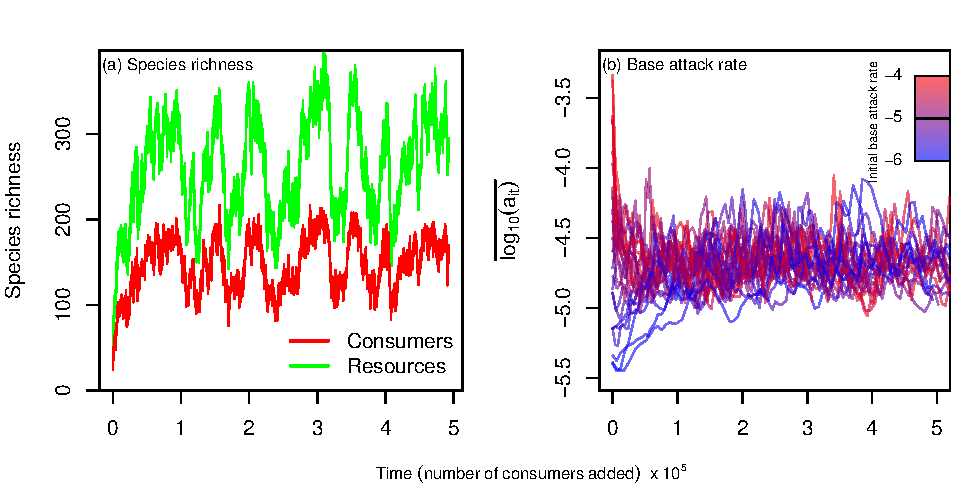
\includegraphics[scale=1]{../Images/spec_a_full.pdf}
 \caption{\label{fig:spec_a_full} Time-series of species richness, panel (a), and average log transformed base attack rates, panel (b). Both figures reach a steady-sate (i.e. when the average value of the time-series becomes time-independent) after around $0.5 \times 10^5$ consumer additions. For panel (a) the red and green graphs respectively represent the number consumers and resources in each time-step of a single assembly model simulation. In panel (b) I have plotted the time-series for many initial base attack rate values used in respective assembly simulations, the colour transitions from blue to red reflects this ascension (as represented by the colour gradient legend on the top right hand-side)}
\end{figure}


\subsection{The curse of complexity}
 Whilst the mechanisms relating to the steady-state of species richness are discussed by \citep{Rossberg2013}, those relating to the steady-state of base attack rates have remained largely opaque. This is due to the problem of intractability associated with identifying each new steady state of this system, which occurs with every new species addition and subsequent numerical integration. Theoretical contributions to the study of ecosystem stability have usually focused on deriving approximate measures that signal the vulnerability of a food-web to undergo a change of state that leads to the loss/extinction of constituent species. As reviewed by \citep{Landi2018}, this can occur for a variety of reasons and are thus classified accordingly. As argued by \citep{Grimm1997} how classifications and measures used to describe changes of state can become ambiguous if they are not used and defined carefully. Some examples of specific studies dedicated to understanding the existence of species richness steady-states and / or the mechanisms driving species extinctions have been discussed using a variety mathematical approaches such as \citep{Rossberg2013}, \citep{Pawar2015}, \citep{Pawar2009}, \citep{Bastolla2005a}, \citep{Bastolla2005b}. They respectively describe and characterise how instability thresholds - where by instability I loosely refer to a loss of species due to any type of extinction - may be calculated for a fixed set of system parameters. These measures are not directly translatable to the focus of this study however: They signal the vulnerability of the whole system to undergo a change of state rather than the propensity for individual species to go extinct, which as I explain in Sec. \ref{sec:evolutionary-forces}, is crucial for understanding the long-term fitness of species, and therefore why species with intermediate base attack rate strength are fittest. \\
 
 One of the most relevant (albeit unusable in this thesis) measures for understanding the propensity of individual species to go extinct, is the weighted generality $G^w_i$ of a species $i$ derived by \citep{Pawar2009}. This measure is derived in a food-web assembly study similar to that defined in Sec. \ref{sec:model_definition}. The only difference other than the parametrisation is the use of carrying capacity for all species and the possibility of omnivory. $G^w_i$ is used to measure the phenotype - such as body-mass as detailed by \citep{Pawar2015} - specific contribution of a species to the total weighted generality, $G^w_{tot}=\sum G^w_i$, of a complex food-web. Given $G^w_{tot}$ is correlated with the real part of the largest eigenvalue $\lambda_{max}(C)$ of the Jacobian (of the interaction matrix), $C$, adding more species increases $G^w_{tot}$ and therefore the chance of the system to loose Routh-Hurwitz stability (it increases the chances of $\lambda_{max}(C)$ becoming positive). Although this measure is used to identify a negative feedback associated with species biomass type in \citep{Pawar2015}, because the total weighted generality is only correlated with the $\lambda_{max}(C)$ (and not any of the other eigenvalues), one cannot interpret the exact nature of the instability, i.e. how many or which species go extinct. Thus whilst the likelihood of an event leading to the loss of species might potentially be inferred from the weighted generality measure in \citep{Pawar2009}, the actual type and number of these (and the resulting negative feedback effect) cannot. \\
 
 Another interesting theoretical study on the effects of invaders on ecosystem stability in species competition model is that of \citep{Barbier2019}. The authors de-couple the per capita change in biomass $\frac{1}{N_i}\frac{\d N_0}{\d t}$ of an invading species $i$ into two components. The first, $w_0$, is the invasion fitness i.e. initial growth of $i$ when it is rare and is yet to significantly alter the biomass of resident species. The second, $v_0$, is the effective density dependence of the invader’s growth rate, which measures the long-term effects of invasion after the biomass of the invader is large enough to affect resident's biomass. The fate of an invasion attempt (either no invasion, coexistence, turnover, irreversible turnover or alternate stable states) is then categorised according to the ratio of $v_0$ and $w_0$. In the supplementary material this is then extended to a resource-consumer model such as the one discussed in this thesis. These results are not directly extendible to the analysis pursued in this thesis however, given they are concerned with understanding the invasive feedbacks of consumer competition resulting from shared resources (i.e. resource mediated competition). This analysis does not account for the potential resource species that are lost, which as I explain in Sec. \ref{sec:cons_lifetime} and show in Fig. \ref{fig:comp_decon}, is crucial for understanding the immediate effects of invasion, and long-term effects resulting from these and from the interaction of other invading resources and consumers.\\

 To understand how consumer feedbacks vary according to species type, one must understand the variation in the likelihood, extent and type of instabilities caused (or propensity to cause them) at the species level. To achieve this, I propose to simplify the different stages of the numerical integration process that relate to species invasions, establishment and turnover. In this way the likelihood, type and resulting negative feedback of instabilities may be mechanistically inferred according to consumer species type (the base attack rate $a_i$). In the following section I will derive and validate these components. The second part of the validation will occur by combining the simplified components into an assembly algorithm (called the deconstructed community assembly algorithm) that mimics the full community model such that it qualitatively reproduces its most important characteristics: The steady-state/steady-state in the time series of species richness and average log transformed base attack rates that are depicted in Fig.~\ref{fig:spec_a_full}. 
 
\section{The deconstructed food-web model}
\label{sec:deconstr-food-web}

In the deconstructed model variant, dynamics following invasions are simplified to a form that avoids simulation of the system of ordinary differential equations Eq. \eqref{eq:LV1}. Instead, dynamics are broken
up into a sequence of phases that permit an approximate analytic description. Each phase can be considered as an independent module (that can be added or removed to the underlying algorithm) that represents particular ecological phenomena. To highlight the similarity of these modules and those considered in invasion ecology (without claiming that they are identical), I name these using analogies to corresponding phases
distinguished and discussed by \citep{Lockwood13:_InvasionEcology} and \citep{Reise06:_AreAliens}. The analogy to invasion ecology becomes clearest if one views the model as describing an ecological community on an island that is occasionally invaded by species from other islands.
\subsection{The deconstructed assembly algorithm}

The aim for the deconstructed model is not to reproduce the dynamics of the full model in all detail but only its system-level phenomenology. For this, surprisingly coarse approximations turn out to be sufficient. All equation references can be found in Box \ref{box:conditions}. Furthermore when I refer to the "main resource" $i$ of a consumer $j$, I am referring to the resource for which $H_{ij}$ is largest over all $i$. The description of the algorithm of the deconstructed
model is as follows:

\begin{enumerate}

\item Initially populate
 an ecosystem with a small set of randomly sampled consumers 
  $S_{\mathrm{C}}=10$ and resources $S_{\mathrm{R}}=20$). The subsequent addition of species, resulting in community assembly and turnover, occurs by:
\item \textbf{Transport (i):} Sample with equal probability whether the next species to invade is a consumer or a resource. \label{step:Ti}
\item If a consumer is to invade, do the following:
\begin{enumerate}
\item \textbf{Transport (ii):} Sample the base attack rate $a_k$ and interaction coefficients $H_{jk}$ for a candidate invader as described in Sec.~\ref{sec:sampling-new-species}.\label{step:Tii}

\item \textbf{Establishment:} Test whether this consumer can invade using first the criterion that the consumer should be able to invade in absence of competitors, Eq. \eqref{eq:invadability_criterion}, and then the (stronger but computationally more expensive) requirement that it should withstand competition from each of the resident consumers $j$ by Eq. \eqref{eq:gen_comp_in}. If it cannot invade, repeat from Step \ref{step:Tii} until a species is sampled that can invade the community. \item \textbf{Spread (within island):} Remove all of the invading consumer's resources that can get over-exploited in the consumer's early boom phase according to Eq. \eqref{eq:overexploitation}.

\item \textbf{Bust after boom:} If the invading consumer now fails the invasibility criterion, Eq. \eqref{eq:invadability_criterion}, remove it and continue with Step \ref{step:adjustment_start}.

\item \textbf{Impact (resource serial extinctions):} If
    Eq. \eqref{eq:serial_extinction} predicts extinction of the
    consumer's main resource by consumer-mediate competition,
    remove that resource and repeat
    Step~3 (e) \label{step:serial_extinction}
  \end{enumerate}
\item If otherwise a producer is to invade, do the following:
  \begin{enumerate}
\item \textbf{Transport (ii):} Sample the producer's interaction
    coefficients $H_{jk}$ as described in
    Sec.~\ref{sec:sampling-new-species} and add it to the
    community\label{step:TiiP}.
\item \textbf{Expansion \& Impact:} While there are consumers
    satisfying the condition for consumer mediated extinction,
    Eq. \eqref{eq:serial_extinction}, repeat the following:
    \begin{enumerate}
    \item Chose one of these consumers at random and call it $l$.
\item Remove $l$'s main resource.
\item Remove any consumers $k$ that now fail
      to satisfy the invasibility
      criterion given by Eq. \eqref{eq:invadability_criterion}.
    \end{enumerate}
  \end{enumerate}
\item \label{step:adjustment_start}\textbf{Adjustment (Exploitative
    competition):} Test which consumers $i$ satisfy the condition for
  exploitative competitive exclusion, Eq. \eqref{eq:gen_comp_in}, by
  any other consumers $j$.  Then remove all that do.
\item \textbf{Adjustment (Pyrrhic competition):} Test which consumers
  satisfy the condition for loss in Pyrrhic competition,
  Eq. \eqref{eq:spec_extinction}, against any other consumers.  Then
  remove \emph{the main resource} of all that do.
\item \textbf{Adjustment:} Remove
  all consumers that now fail the invasibility criterion given by
  Eq. \eqref{eq:invadability_criterion}.
\item Repeat from Step~\ref{step:Ti}.
\end{enumerate}

\newpage

\begin{floatbox}
  \caption{The simplified criteria for the processes structuring
    predator-prey communities used in the deconstructed model presented as respective modules. The corresponding derivations are provided in the sections \ref{sec:inv}\ref{sec:res_over}, \ref{sec:ser_ext}, \ref{sec:exp_comp} and \ref{sec:phy_comp}}.\label{box:conditions}
% \paragraph*{Simplification of ``Establishment'': Respiration and consumer competition
% as invasion criterions.}

\textbf{Invasibility criterion} (simplified by setting $B_{k}^{\mathrm{R}}=K=1\,\forall k$):

\begin{equation}
\sum_{k=1}^{S_{\mathrm{R}}}H_{ki}-1>0\label{eq:invadability_criterion}
\end{equation}
\textbf{Exploitative competition} leading to exclusion of consumer $i$
by consumer $j$:
\begin{equation}
 \sum_{k=1}^{S_{\mathrm{R}}}H_{ki}<1+
 \left(
   \sum_{k=1}H_{ki}H_{kj}
\right)\frac{(\sum_{k=1}H_{kj}-1)}{\sum_{k=1}H_{kj}^{2}}\label{eq:gen_comp_in}
\end{equation}

\textbf{Overexploitation} of resource $k$ during spread of consumer
$i$:
\begin{equation}
\ensuremath{H_{ki}\geq \log\left(\frac{K}{B_{\text{min}}}\right)}\label{eq:overexploitation}
\end{equation}
\textbf{Serial extinction} induced by consumer mediated (``apparent'') competition} leading to loss
of main resource of consumer $k$:
\begin{equation}
  \left(
    \sum_{k=1}^{S_{\mathrm{R}}}H_{ki}-1
\right)>\frac{\sum_{k=1}^{S_{\mathrm{R}}}H_{ki}^{2}}{\max_{k}(H_{ki})}\label{eq:serial_extinction}
\end{equation}
\textbf{Phyrric competition} between consumers $i$ and $j$ leading to
extinction of $i$'s main resource $k$:
\begin{equation}
  H_{ki}<H_{kj}\label{eq:spec_extinction}
\end{equation}
\end{floatbox}

\subsection{Comparison of macroscopic features of full and deconstructed community models}
\label{sec:results}


To see how well the deconstructed model reproduces the long-term
dynamics of the full model with explicit simulation of population
dynamics, I ran both models with the same set of parameters, as given in
Table \ref{tab:parameters}. As shown in Fig.~\ref{fig:spec_rich_time},
the richness of consumers ($S_C$) and resources ($S_R$) rises in both
models until about $0.5\cdot 10^5$ consumers have been iteratively
added, and then fluctuates around some long-term average value.
Species richness in the deconstructed model tends to be slightly
higher, but by and large the deconstructed model reproduces the
richness values obtained using the full model.\\

 I demonstrate for both models that community mean logarithmic base attack rates
$\overline{\log_{10}(\alpha_0 a_{i})}$ reach a steady state over the
same initial period of about $0.5\cdot 10^4$ consumer invasions and then
fluctuate around long-term mean (Fig.~\ref{fig:agg-through-time}), and that this steady state is independent of the value of base attack rate chosen for the initial set of
consumers. In the deconstructed model steady-state base attack rates
tend to be slightly higher than in the full model. The mean over the simulation used to create Fig. \ref{fig:agg-through-time}) of
$\overline{\log_{10}(\alpha_0 a_{i})}$ across time
($2$--$5\cdot 10^{5}$ consumer additions) is
$10^{-4.75}$ for the full model, and $10^{-5.25}$ for the deconstructed model. To understand how this equilibria varies from a null expectation (i.e. one in which no selection is occurring) we can compare this values to the expected value of scaled attack rates given by
Eq. \eqref{eq:attack-rate-sampling}. This can be calculated using the identity for the expectation of log-normally distributed random variables
\begin{equation}
\mathsf{E}\big[a e^{\mu+\sigma Z}\big]=a e^{\mu+\frac{\sigma}{2}},
\end{equation}
where $Z$ is a standard normal random variable and is exactly equivalent to the distribution of $\xi_{ki}$. Here $\mu$ is the shift in mean of $Z$ (which is equal to zero in Eq. \eqref{eq:attack-rate-sampling}) and $\sigma$ represents the standard deviation of the resulting $\mu+\sigma Z$ distribution, equivalent to the inverse niche width $\sigma$ parameter in Eq. \eqref{eq:attack-rate-sampling}. We then have $\mathsf{E}[H_{jk}]= \alpha_0 a_k e^{\sigma^2/2}$, which evaluates to about $\alpha_0 a_k 10^{5.4}$ for our choice of $\sigma$. This implies
that that average scaled attack rates reach equilibria at values of
the order of magnitude of one in both model variants. \\

\begin{figure}[H]
% Graph created in final_paper_graphs_2.R
\centering{}
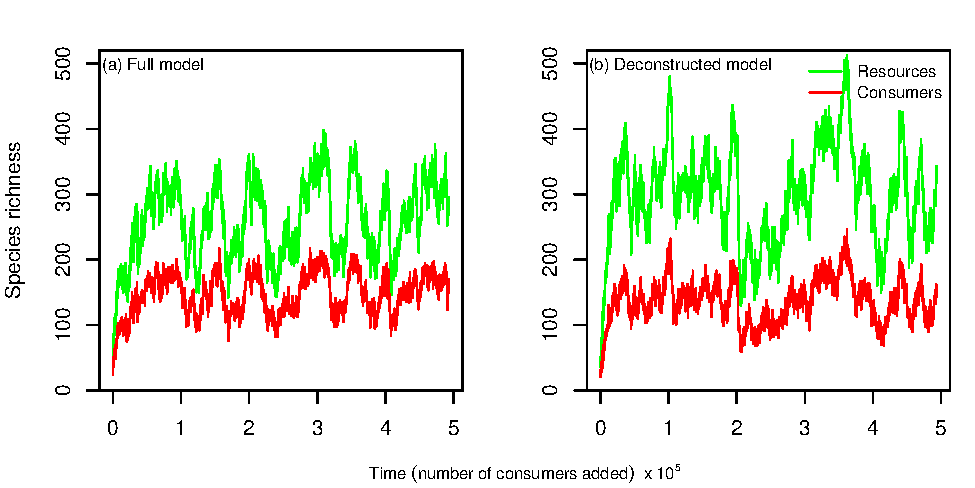
\includegraphics[scale=1]{../Images/animal_plants.pdf}
\caption{Comparison of the species richness time-series of consumers $S_C$ (red) and resources $S_R$ (green). A steady-state is reached for both full (a) and deconstructed (b) assembly models when species richness fluctuates around a constant mean. The average number of species during the steady state is slightly larger for the deconstructed model. \label{fig:spec_rich_time}}
\end{figure}\\

\begin{figure}[H]
% Graph created in final_paper_graphs_2.R

\centering{}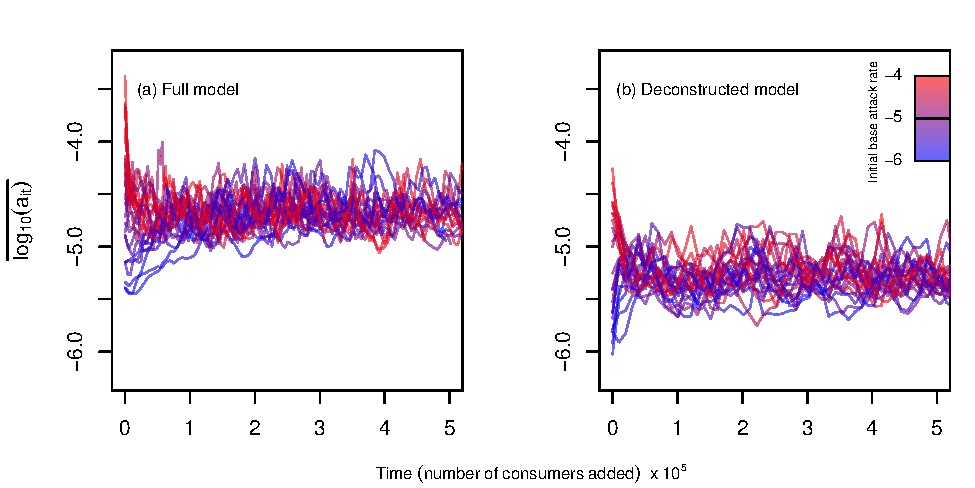
\includegraphics[scale=1]{../Images/agg_time_series.pdf}
 \caption{ Comparison of the time-series of $\log(\overline{a_{i}})$
    for the (a) full and (b) deconstructed models. The mean of the deconstructed model is larger than full model's by an order of magnitude of roughly 0.5. For both models the respective steady state is reached independently of the initial conditions tested for.\label{fig:agg-through-time}}
\end{figure}


\subsection{Invasibility criterion} \label{sec:inv}

I will now provide the derivation and validation for the modules used in the deconstructed model. The invasibility criterion is used in many theoretical and empirical studies of ecology (see \citep{Pawar2009} for an example of how it is used in a theoretical setting similar this study). It is derived by finding for which conditions will Eq. \eqref{eq:LV_resource1} be positive for a mutant species attempting to invade with attack rate $a_{m}$:

\begin{equation}
\sum_{k=1}^{S_{\mathrm{R}}}\epsilon a_{km}B_{k}^{R}>\rho. \label{eq:invadability_criterion_2}
\end{equation}

The invasibility criterion therefore states an invasion attempt can be characterised by the ability of a species to acquire enough biomass from trophic interactions (as given by the left-hand side of Eq. \eqref{eq:invadability_criterion_2}) so it may overcome respiration (the right hand side of Eq. \eqref{eq:invadability_criterion_2}). The criterion also implies that one may ignore competition with other residents mediated by shared resources, and the competition between resources mediated by their shared consumer. To construct Eq. \eqref{eq:invadability_criterion} I approximate $B_{k}^{R}$ by the carrying capacity $K$ in Eq. \eqref{eq:invadability_criterion_2} and divide by $\rho$ which subsequently yields Eq.  \eqref{eq:invadability_criterion}. To validate the use of this module, and indeed the underlying assumptions (i.e. that species invasions can be approximated via \eqref{eq:invadability_criterion}) I firstly calculate the numeric estimate of the invasion probability. I achieve this using steps 3.a and 3.b of the deconstructed assembly algorithm (and analogous steps of the full assembly model), such that I estimate the invasion probability of a mutant with base attack rate $a_m$ for a fixed range of base attack rates (as depicted in Fig.  \ref{fig:birth_verification}) and a fixed number of invasion attempts. The numeric estimate for each base attack value is calculated by recording the proportion of successful invasion attempts, where success is strictly defined as the ability to initially invade, i.e. achieve positive growth at the point of invasion. Even if a consumer were to go extinct after the initial invasion, during the establishment phase, this is still considered a successful attempt to invade the food-web. Fig.\ref{fig:birth_verification}) shows us that the approximated numeric invasion probability obtained using Eq. \eqref{eq:invadability_criterion_2} qualitatively resembles that obtained by numerically simulating species invasions in food-webs generated using the full assembly model. This approximation is improved by correcting the assumption that $B_{k}^{R} \approx K$ $\forall k$ to $B_{k}^{R} \approx \overline{B_{k}^{R}}^{*}$ $\forall k$ in Eq. \eqref{eq:invadability_criterion_2} (i.e. that biomasses of resident resources should be approximated by their average value at equilibrium rather than their carrying capacity). \\

% Graph created in invasion_prob_test_2.R
\begin{figure}[H]
 
\centering{}
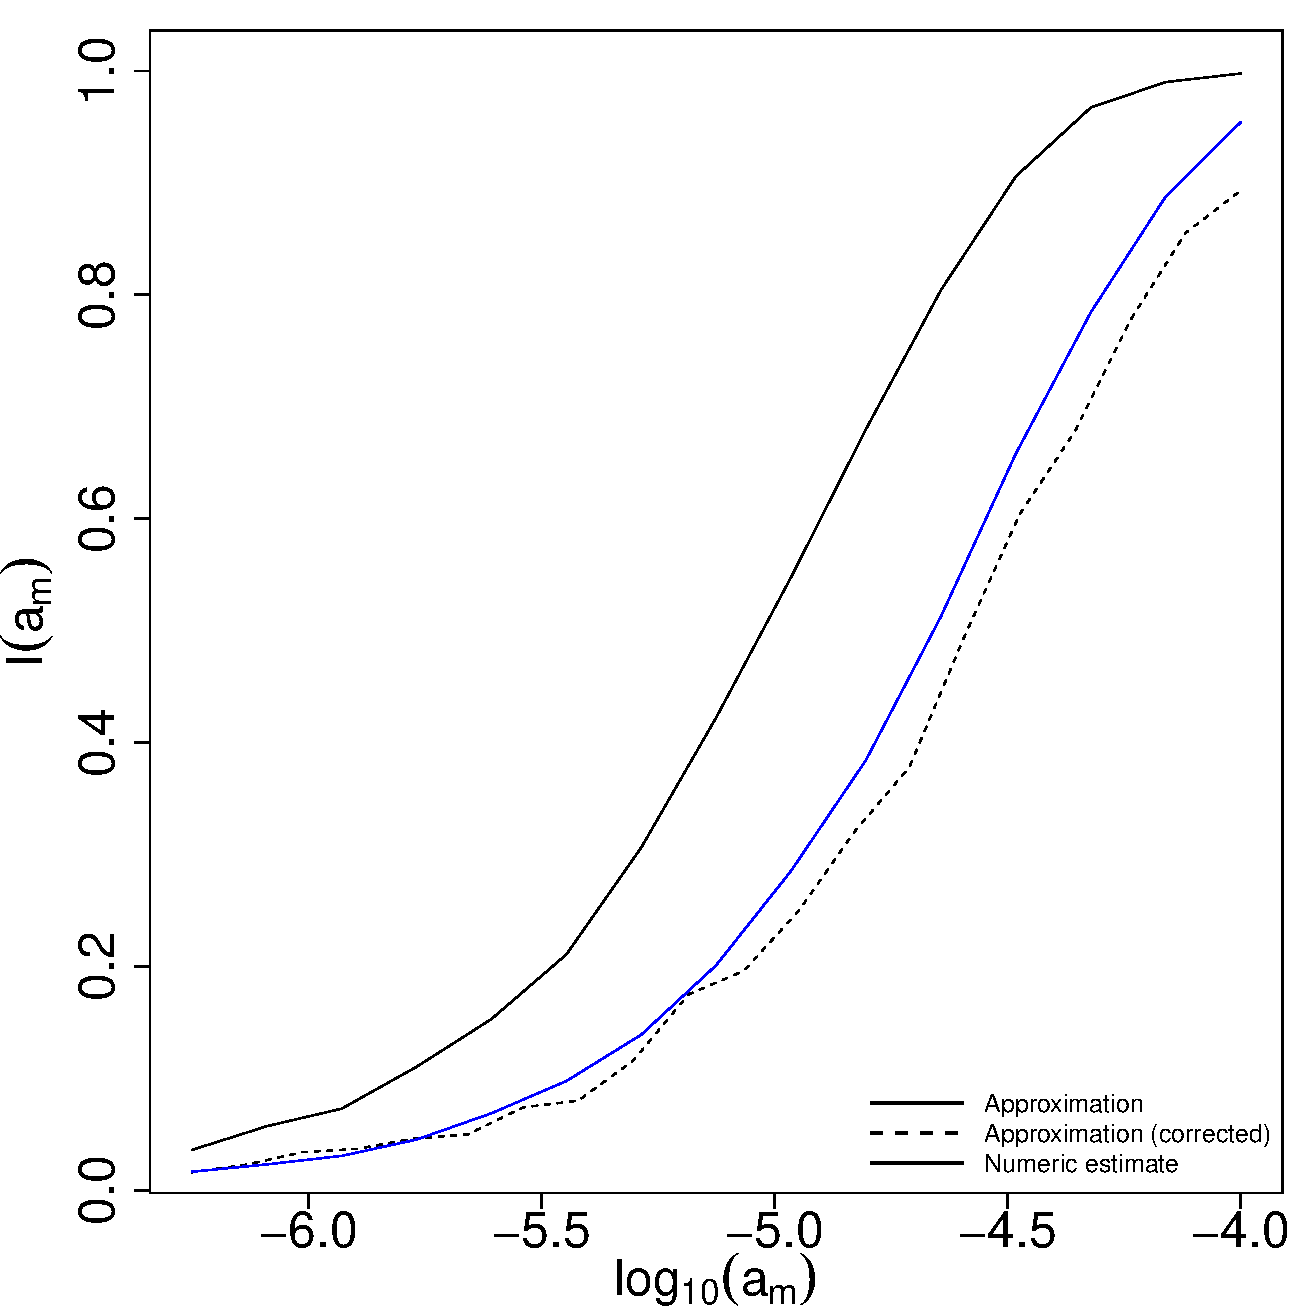
\includegraphics[scale=0.5]{../Images/Invasion_verification.pdf}
 \caption{Numeric estimates of simulated (blue) and approximated (black - using Eq. \eqref{eq:invadability_criterion_2}) invasion probabilities (y-axis) as functions of mutant's base attack rates $a_m$ (x-axis) attempting to invade a food-web. For the simulation estimate (blue) I randomly sampled 100 food-webs saved during the simulation of the assembly food-web. For each base attack rate value (ranging between $10^{-6.25}-10^{-4}$) I then calculated the proportion of successful invasions out of 1000 attempts per food-web. For the approximated estimated probability (black) I fix the number of resource to be the average number of resources at equilibrium (roughly $S_R=250$ resources). For the same range of base attack rates used for the simulation estimate, I then calculated the proportion of successful approximated invasions out of 10000 attempts (sampling an independent set of trophic links at each attempt) by summing the number of times Eq. \eqref{eq:invadability_criterion_2} was satisfied. I improved this approximation (black dotted line) by correcting the carrying capacity by adjust the carrying capacity as $K=\overline{B_{k}^{R}}^{*}$ in Eq. \eqref{eq:invadability_criterion_2} (where $B_{k}^{R}$ is the average resource biomass at equilibrium). 
\label{fig:birth_verification}}
\end{figure}
 
\subsection{Resource Overexploitation}
\label{sec:res_over}
This module simplifies the removal of resources $k$ of a mutant consumer $m$ if the underlying attack rates would lead to the extinction of that resource during the invasion of the mutant. It is possible that during the invasion of a consumer, the biomass of a resource may drop below the extinction threshold, and should therefore be removed. This can occur even though a resource may achieve an equilibrium biomass above the extinction threshold at equilibrium. I use the approximation found in \citep{Rossberg2013} that firstly reduces food-web complexity by only considering the individual pairing of each consumer and resource, as if the former relied only on the latter in isolation. In this scenario, if the resource risks extinction, its biomass will be so low that the self-limiting term in \eqref{eq:LV_resource1} becomes negligible, such that the dynamics of consumer and resource are reduced to the classic Lotka-Volterra equations. The resource minimum biomass value reached is approximately $K \exp(-H_{k,m})$. If $H_{k,m}$ is such that $K e^{-H_{k,m}}$ falls below the extinction threshold $B_{\text{min}}$, resource $k$ should be removed from the system, i.e. if $K \exp(-H_{k,m})<B_{\text{min}}$ which can be re-arranged in terms of $a_{k,m}$

\begin{equation}
a_{k,m}\geq a_{crit}=\frac{\log(\frac{K}{Mmin})\rho}{K\epsilon}.\label{eq:over_exploitation}
\end{equation}

This module assumes that other direct/indirect effects 
of other trophic interactions not considered Eq. \eqref{eq:over_exploitation} do not significantly alter the fate of resource deemed to go extinct according to Eq. \eqref{eq:over_exploitation}, and that it is bound to go extinct. Numerical validation is provided by firstly assuming that for an invasive consumer species $i$, if one of its trophic links satisfies were strong enough to cause the extinction of a resource $k$ (such that if the food-web were solely composed by that resource species $k$), then no other interaction (either direct with other resources or indirect with other consumers) will be able to stop the extinction of $k$. To validate this module I may continue by simplifying the food-web such that it is composed solely of one resource, and safely assume that extrapolating it to any other more complex food-web will not affect the fate of the resource. To continue, I calculate the minimum biomass of a resource, $\min_{t} B^R(t)$), of the sole resource species in a food-web, during the invasion of an invasive consumer species $i$. I calculated $\min_{t} B^R(t)$ as a function of $\omega$, such that $a_{k,i}=\omega a_{crit}$, i.e. the trophic link of the invader is a fraction $\omega$ of the strength expected to cause the extinction of the resident. I did this for different initial values $B^R(0)$ of the resident resource species to show how the approximation of Eq. \eqref{eq:over_exploitation} varies with the initial value of the resource (which would of course vary if we were to replicate the experiment in a simulated food-web with many resource consumers and resources). We can see that the approximation decreases in accuracy as $B^R(0)$ decreases. The actual average value of $B^R(0)$ in the full assembly model is approximately 0.5. According to Fig. \ref{fig:res_over} we should therefore expect the value $\omega\approx 1.3$ to be occurring on average in full assembly model simulation. Thus the approximation I implement for the deconstructed model (i.e. where $\omega=1$) is well within the order of magnitude of occurring on average.

\begin{figure}[H]
\centering{}
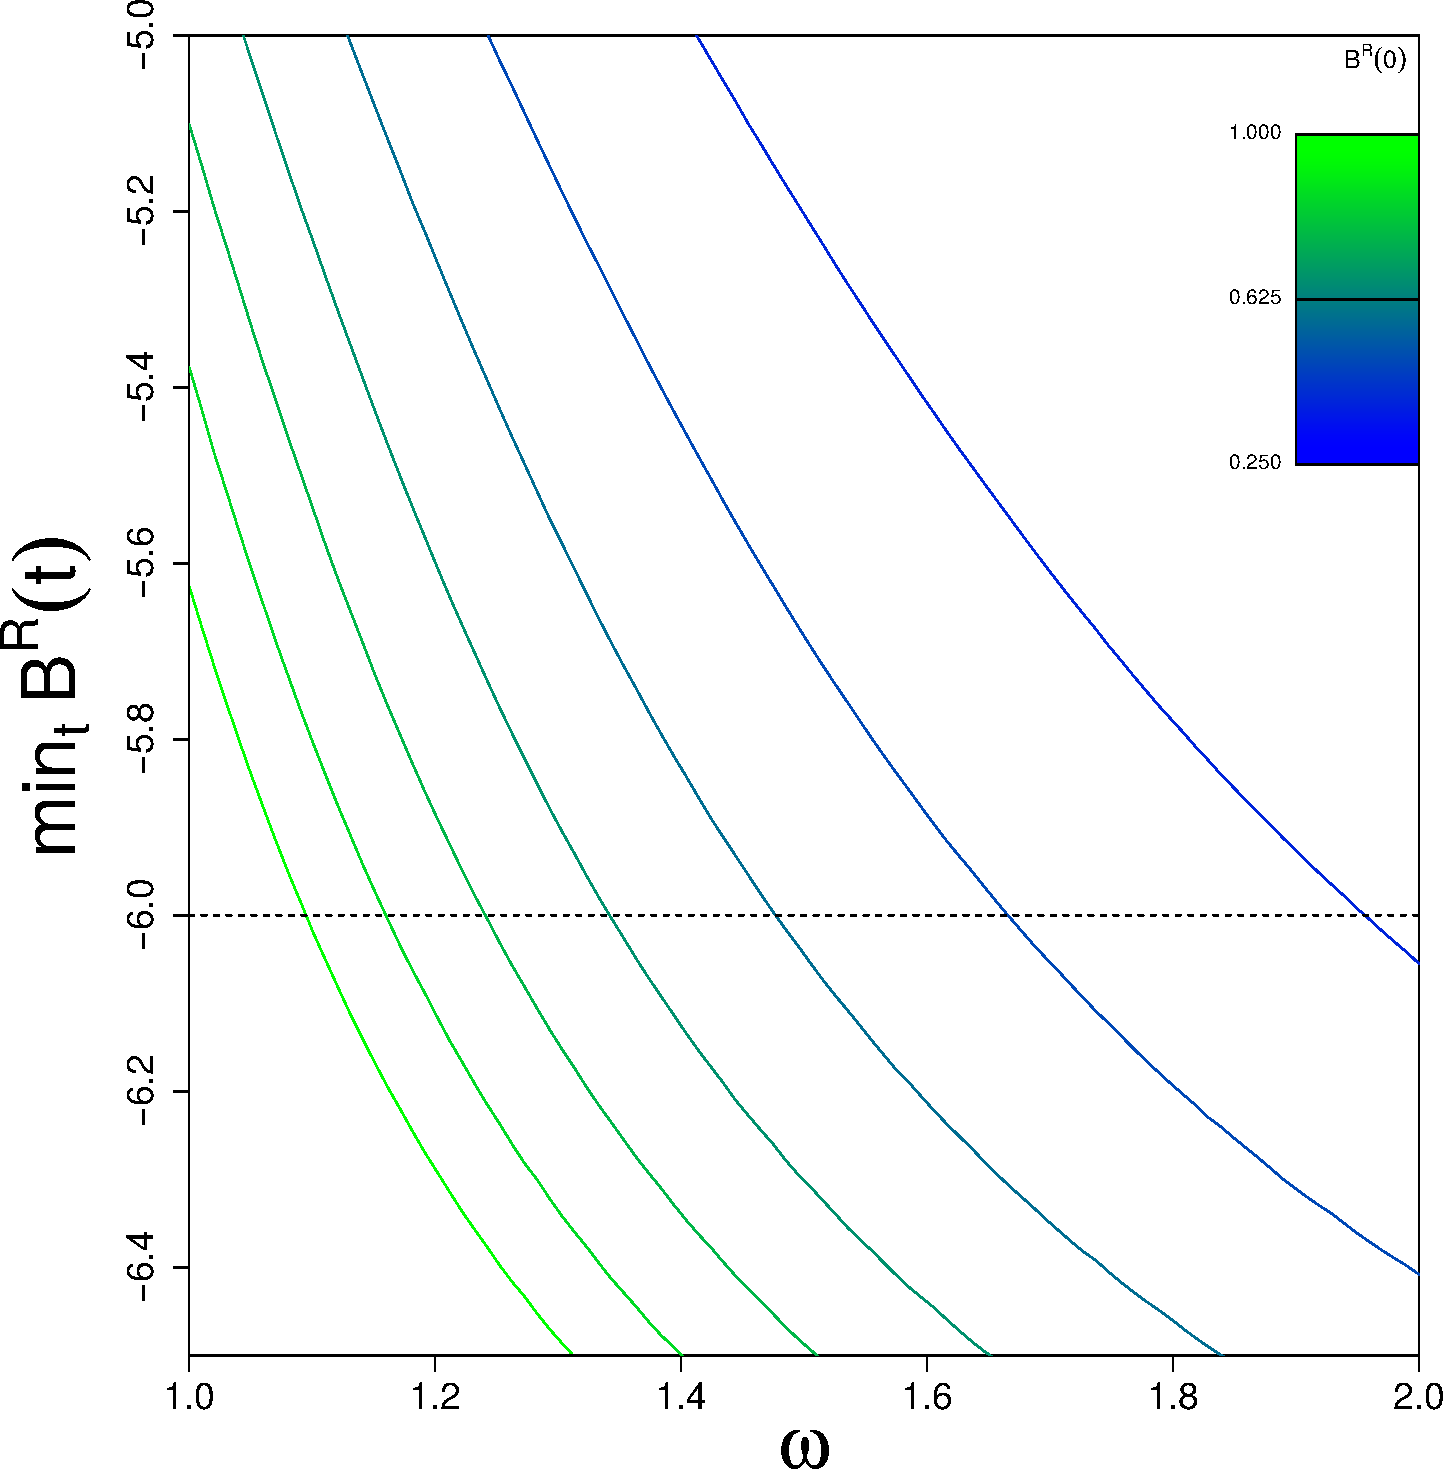
\includegraphics[scale=0.5]{../Images/Over_exploitative.pdf}
\caption{The minimum biomass of a resource, $\min_{t} B^R(t)$ (the sole species in a food-web) during the invasion of the invasive consumer species $i$ as a function of a dimensionless scaling factor, $\omega$ (where $a_{k,i}=\omega a_{crit}$). The ascending colour progression from green to blue represents the increase in the initial value $B^R(0)$ at which the invading consumers attempts to establish itself (the initial biomass of the invader is that used for the full food-web assembly). The dashed black line represents $B_{min}$, the expected value of $\min_{t} B^R(t)$ that should be reached according to the resource overexploitation module. As we can see, to reach this value, we must increase $\omega$ as we decrease $B^R(0)$.
\label{fig:res_over}}
\end{figure}

\subsection{Serial extinctions}
\label{sec:ser_ext}

The theory of apparent competition, as coined by \citep{Hold1977}, states that "alternate prey species in the diet of a food-limited generalist predator should reduce each other's equilibrial abundances, whether or not they directly compete". Any such reductions in abundance that mathematically fall below zero should therefore be accounted for in the deconstructed model. I use the serial extinction inequality to achieved this, provided by \citep{Rossberg2013}, that models the change in the biomass of resources, by ignoring the effects of all other resident consumers. This simplification again assumes that competition between consumers is weak, such that consumers do not share important resources, and that resources equilibrium biomasses are close to carrying capacity. Re-arranging the general equilibrium for this simplified system generates resource biomasses as:

\begin{equation}
B_j^R = \Big(1-\frac{H_j\sum_{k=1}^{S_R}H_k}{\sum_{k=1}^{S_R}H_k^2} + \frac{H_j}{\sum_{k=1}^{S_R}H_k^2} \Big)
\end{equation}

such that if for any resource $j$

\begin{equation}
\label{eq:just_b_ser_ext}
\Big(\sum_{k=1}^{S_{R}}H_{k,i}-1\Big)H_j-\sum_{k=1}^{S_{R}}(H_{k,i})^{2}\geq 0
\end{equation}

is satisfied, resource $j$ will go extinct. Given that for each resource subtraction $j$, it is not guaranteed Eq. \eqref{eq:just_b_ser_ext} will still be satisfied for other resources $l$ that also satisfied Eq. \eqref{eq:just_b_ser_ext} prior to the removal of $j$, one should re-establish the serial extinction as
\begin{equation}
\Big(\sum_{k=1}^{S_{R}}H_{k,i}-1\Big)H_{max,i}-\sum_{k=1}^{S_{R}}(H_{k,i})^{2}\geq 0, \label{eq:serial_cond}
\end{equation}

and only remove the resource link corresponding to $H_{max,i}$ of a consumer $i$ (given that this is the most likely the first resource to cross the extinction threshold). Eq. \eqref{eq:serial_cond} should then be re-calculated for every resource that is removed from the food-web until no more resources go extinct via this mechanism. 


\subsubsection{Serial extinction validation algorithm \label{sec:serial_ext}}

To ensure that the analytic derivation of the resource extinction procedure given by Eq. \eqref{eq:serial_extinction} is correct, one could could compare the resources predicted to go extinct versus the actual resource turnover in the full assembly model. However given species go extinct for reasons other than serial extinction, one cannot directly prove that any resource that does go extinct is specifically due to the prediction of Eq. \eqref{eq:serial_extinction}. Therefore, to ensure an experimental set up in which resources extinction can only occur due to the serial extinction process, I created a sub-model of the ordinary differential equation full assembly model using Eq. \eqref{eq:LV_consumer1} $\&$ Eq. \eqref{eq:LV_resource1} in which only one consumers feeds on a set of resources. In this way resources may only go extinct because of the foraging intensity of the consumer. I then compared the sum of trophic links $\ln\(\sum_{k=1}^{S_{R}}H_{k,i}$ resulting from the repeated addition of resource species (which may or may not active the serial extinction process) to the predicted value that uses Eq. \eqref{eq:serial_extinction} to potentially remove resources. I chose $\ln(\sum_{k=1}^{S_{R}}H_{k,i})$ as a focal comparison point because it controls the invasion fitness of consumers in the absence of competitors. For each fixed base attack rate value I

\begin{enumerate}
\item Sample a set of $S_R$ trophic links conditional to a consumer $i$ being capable of overcoming respiration according to Eq. \eqref{eq:invadability_criterion} by ensuring $i$'s biomass increases after integrating the one consumer and $S_R$ resource food-web after a few time-steps.

\item Create a copy of the set of trophic links such that $H^F_i$ represents the set of links belonging to the full model and $H^D_i$ represents that of the deconstructed model.

\item For $H^D_i$, remove the maximal link of  until Eq. \eqref{eq:serial_extinction} is satisfied. 

\item For $H^F_i$, construct a coupled Lotka-Volterra systems composed of one consumer and $S_R$ resources using Eq. \eqref{eq:LV_consumer1} $\&$ Eq. \eqref{eq:LV_resource1} and integrate for 2000 time-steps (i.e. until equilibrium is reached). Remove any resources whose biomass fall below the extinction threshold $B_{\text{min}}$.

\item If any resources have been lost for either $H^D_i$ or $H^F_i$, such that the resultant number of trophic links is less than $S_R$, re-sample the number of lost trophic links and add these to the respective full and deconstructed food-web. If no links were lost, choose a link at random and replace it by sampling a new one, ensure the consumer can overcome respiration according to Eq. \eqref{eq:invadability_criterion}. 

\item Repeat steps 3. 4. and 5. for each fixed base attack rate value $N$ times to obtain one replicate for the change in $H^D_i$ and $H^F_i$ for a hypothetical turnover of the resource community.
\end{enumerate}

% Graph created in final_graphs_2.R
\begin{figure}[H]

\centering{}
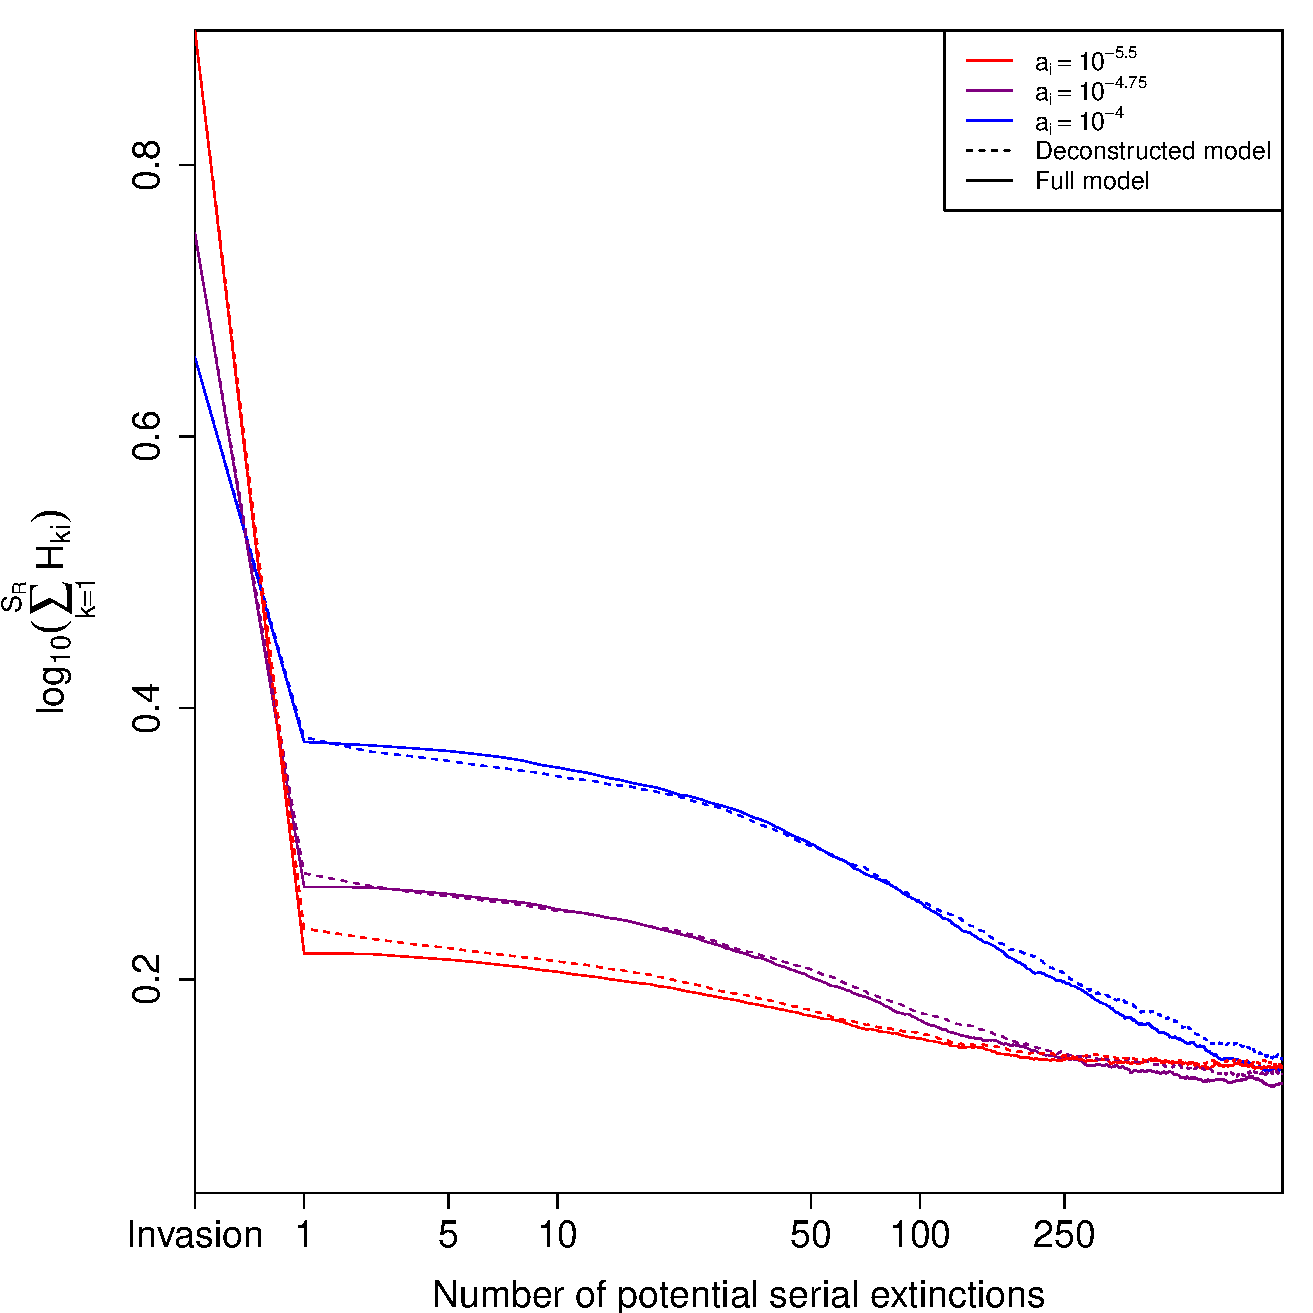
\includegraphics[scale=0.5]{../Images/serial_extinction.pdf} \caption{Depiction of the change (y-axis) in $\log_{10}(\sum_{k=1}^{S_R}H_{ki})$ (a quantity that controls invasion fitness in absence of competitors given it is contained in the invasibility criterion given by Eq. \eqref{eq:invadability_criterion}) according to the serial extinction validation algorithm that cumulatively adds $N$ resource additions (x-axis) described in Sec. \ref{sec:serial_ext}, averaged over 1000 replicate consumers. Each colour represents a distinct fixed value ($10^{-5.5}$, $10^{-4.75}$ and $10^{-4}$) of base attack rate ascending from blue to red. For each replicate I focus on a consumer $i$ and sample $S_R=300$ initial trophic links. The initial set of resources required to overcome respiration is denoted as “Invasion” on the x-axis. The full model curves (dashed lines) correspond to values of $H^F_i$ in which the biomass of species is obtained via numeric integration using ODE solver function “ode” in the “deSolve” R package (using the default solve method and tolerance setting, and 5000 maximal integration steps). The Deconstructed model curves (solid lines) correspond to values of $H^D_i$ in which resources were removed using the serial extinction inequality given by Eq. \eqref{eq:serial_extinction}.\label{fig:serial_ext}}
\end{figure}

In Fig.~\ref{fig:serial_ext} we see that although species with larger base attack rates initially have a larger sum over trophic links at the point of invasion - denoted by "Invasion" in Fig.~\ref{fig:serial_ext}) - after establishment - indicated by "1" Fig.~\ref{fig:serial_ext} - this hierarchy is reversed: Consumers with larger base attack rates now have a smaller sum over all trophic links. As more resources are added and serial extinction is potentially activated, this hierarchy is maintained until the sum over trophic link slowly becomes virtually independent of the base attack rate $a_i$. The initial change in hierarchy immediately after establishment can be explained by imagining two consumer species $i$ and $j$ that have an identical set of trophic links $\sum_k^{S_R}e_{ki}=\sum_k^{S_R}e_{kj}$ (where $e_{jk}=\frac{a_{kj}}{a_j}=\exp(\sigma \xi_{kj})$, i.e. the trophic link strength divided by the base attack rates) but $a_i<a_j$. If we factor out $\alpha_i$ and $\alpha_j$ from Eq. \eqref{eq:serial_extinction} it can be expressed as 
\begin{equation}
\sum_{k=1}^{S_{R}}e_{k,i}-\frac{\sum_{k=1}^{S_{R}}e_{k,i}^{2}}{e_{max,i}}\geq \frac{1}{\alpha_i}\label{eq:serial_ext_2}
\end{equation}

At the point of invasion, the left hand-side of Eq. \eqref{eq:serial_ext_2} will be exactly equal for both $i$ and $j$. However, the underlying inequality is more likely to be satisfied as $a_i$ increases, and therefore as $\frac{1}{\alpha_i}$ decreases. Larger $a_i$ therefore indicates a larger propensity to loose $e_{max,i}$. This does not imply that the resulting sum of trophic links $i$ will be larger than $j$'s. If we consider the scenario in which $j$ activated the serial extinction $N_j$ times and $i$ only $N_i$ times ($N_j>N_i$ and $a_j>a_i$) then to satisfy $\sum_{k=1}^{S_{R}-N_j}H_{k,i}>\sum_{k=1}^{S_{R}-N_i}H_{k,j}$ we must have
\begin{equation}
 \frac{\sum_{k=1}^{S_{R}-N_i}e_{k,i}}{\sum_{k=1}^{S_{R}-N_j}e_{k,j}} > \frac{\alpha_j}{\alpha_i}. \label{eq:serial_ext_3}
\end{equation}

Therefore as long as the ratio of truncated distribution is larger than the ratio of $\alpha$, smaller base attack rates will have a larger sum over trophic links. According to Fig. \ref{fig:serial_ext}, these cases do occur over the range studied in the community assembly model. \\

\subsection{Exploitative competition}
\label{sec:exp_comp}

Exploitative competition refers to the decrease in abundance for a pair of species $i$ and $j$, driven by the increase in predation pressure on a shared common resource $k$. This phenomenon was first mathematically derived by \citep{schoner1976} and verified experimentally by \citep{Jensen1987} for a pair of species whose dynamics are governed and intrinsically limited via logistic growth. Although in this community assembly model, consumers are not directly limited by logistic growth (they are limited indirectly via their resources), the effect is the same: Species competing for resources may lower one another's biomass, such as to lead to the extinction of the other. The most simple case similar to ours is that of pure competitive exclusion first formally derived by \citep{Hardin1960}, which states that for a pair of species foraging on a self-limiting resource, the species with lower foraging rates will outcompete the other. This type of exclusion may also be occurring in the community assembly model studied here via the mediation of many shared resources. In \citep{Rossberg2013} this is referred to as resource mediated competition, such that for a pair of consumers $i$ and $j$, if one is more efficient at using the shared pool of resources it may outcompete the other. The secondary effect of other consumers other than $i$ and $j$, which will also be competing for the same pool of resources, may either dampen or exacerbate these effects. Trying to include all of these effects into the calculation of equilibrium solution is intractable, thus I proceed by only considering simplified sub-components of the food-web, whereby each component is composed of a pair of consumers and all their shared resources. The underling assumption is that it is unlikely that three or more consumers all compete for similar resources. This assumption is partially empirically motivated and validated by \citep{Pawar2019}. The authors only consider the population dynamics of pairs of predator and prey modelled using coupled differential equations similar to Eq. \eqref{eq:LV_consumer1} and Eq. \eqref{eq:LV_resource1}. Although they only use predator-prey pairings to calculate equilibrium biomasses, instead of considering whole ecosystems, they are able to predict ranges of predator-prey body-mass ratios that should are observed in nature. If consumer competition were such that many consumers competed heavily for shared resources, the prediction used in \citep{Pawar2019} based on simplified predator-prey dynamics should not be effective. To achieve the simplification we require the vector of the linearised equilibrium biomass $b^{C}$ of $S_{C}$ consumers in
a food-web described by Eq. \eqref{eq:LV_consumer1} competing for $S_{R}$
resources described by Eq. \eqref{eq:LV_resource1} can be shown by \citep{Rossberg2013}
to be $b^{C}=(\hat{C^{c}})^{-1}\hat{s}$ where $\hat{C^{c}}=\epsilon A^{T}(C^{P})^{-1}A^{'}+C^{c}$
and $\hat{s}=\epsilon A^{T}(C^{P})^{-1}S^{P}-\rho$. Here $\rho$ is the
vector of respiration parameters for each consumer $i$, $A$ is the
bipartite $S_{R}\times S_{C}$ interaction matrix, $C^{R}$ and $C^{C}$
are matrices of the explicit competition between resources and consumers
of size $S_{R}\times S_{R}$ and $S_{R}\times S_{C}$ respectively.
For the case that $A_{ij}=a_{i}e_{ji}=a_{i}e^{\epsilon_{ji}}$, we
can write the vector of effective growths $\hat{s}$ as
\begin{equation}
\hat{s}_{i}=\epsilon\frac{K}{r}r\sum_{k=1}^{S_{R}}a_{i}e_{ki}-\rho=\rho(\alpha_{i}\sum_{k=1}^{S_{R}}e_{ki}-1)=\rho(H_{i}-1)
\end{equation}
where $H_{i}=\alpha_{i}\sum_{k=1}^{S_{R}}e_{ki}$, $\alpha_{i}=\frac{K\epsilon a_{i}}{\rho}$,
$e_{ki}=e^{\sigma\xi_{ki}}$ and $\xi_{ki}\sim N(0,1)$. For the effective
competition term $\hat{C^{c}}$ I therefore have
\begin{equation}
\hat{C_{ij}^{c}}=\epsilon\frac{K}{r}a_{i}a_{j}\sum_{k=1}e_{ki}e_{kj}=\frac{\rho}{r}\alpha_{i}a_{j}\sum_{k=1}e_{ki}e_{kj} \label{eq:post_sem_def}
\end{equation}
\begin{equation}
\hat{C_{ii}^{c}}=\epsilon\frac{K}{r}a_{i}^{2}\sum_{k=1}e_{ki}^{2}=\frac{\rho}{r}\alpha_{i}a_{i}\sum_{k=1}e_{ki}^{2}.
\end{equation}

 For $S_{C}$ consumers and $S_{R}$ resources such that $i,j\in(1,S_{C})$
and $k\in(1,S_{R})$ then:\\

\begin{center}
$\hat{C^{c}}=\frac{\rho K}{r} \begin{pmatrix}
\alpha_{1}a_{1}\sum_{k=1}e_{k1}^{2} & ... & \alpha_{1}a_{S_{C}}\sum_{k=1}e_{k1}e_{kS_{C}} \\
\vdots & \ddots & \vdots \\
\alpha_{S_{C}}a_{1}\sum_{k=1}e_{kS_{C}}e_{k1} & ...& \alpha_{S_{C}}a_{S_{C}}\sum_{k=1}e_{kS_{C}}^{2}
\end{pmatrix}$
\end{center}

The difficulty arises when calculating $(\hat{C}^{C})^{-1}$, I therefore simplify the problem to that of two consumers competing
over $S_{R}$ resources such that
\begin{center}
$(\hat{C}^{C})^{-1}=\frac{\rho K}{det(\hat{C^{c}})r}\begin{pmatrix}\alpha_{2}a_{2}\sum_{k=1}e_{k2}^{2} & -\alpha_{1}a_{2}\sum_{k=1}e_{k1}e_{k2}\\
-\alpha_{2}a_{1}\sum_{k=1}e_{k1}e_{k2} & \alpha_{1}a_{1}\sum_{k=1}e_{k1}^{2}
\end{pmatrix}$.
\end{center}
I can now obtain $b_{1}^{C}$, the biomass of a focal consumer, which
is simply the first row of $(\hat{C^{c}})^{-1}\hat{s}$):
\begin{equation}
B_{1}^{C}=\frac{\rho^{2}}{det(\hat{C^{c}})r}a_{2}[\alpha_{2}(H_{1}-1)\sum_{k=1}e_{k2}^{2}-\alpha_{1}(H_{2}-1)\sum_{k=1}e_{k1}e_{k2}.]\label{eq:simpli_gen_comp}
\end{equation}
If I wish to know whether the biomass will be negative, we
can ignore $\frac{\rho^{2}}{det(\hat{C^{c}})r}a_{2}$ (given that Eq. \eqref{eq:post_sem_def} implies that the determinant
of a positive-definite matrix is always positive) and focus on the
terms inside the bracket of Eq. \eqref{eq:simpli_gen_comp} which will be negative if 
\begin{equation}
 \sum_{k=1}^{S_{\mathrm{R}}}H_{ki}<1+
 \left(
   \sum_{k=1}H_{ki}H_{kj}
\right)\frac{(\sum_{k=1}H_{kj}-1)}{\sum_{k=1}H_{kj}^{2}}\ \label{eq:exploitative}
\end{equation}

thus verifying Eq. \eqref{eq:gen_comp_in}.

\subsubsection{Validating the exploitative competition module}

As with the other modules, the validation procedure is difficult to implement using the full assembly model because one cannot be sure for which reason species go extinct. I have therefore set up a specific sub-model that tests how food-web complexity affects extinctions that are predicted by Eq. \eqref{eq:exploitative}. The model begins with two consumers competing over a fixed set of resources, conditional to one of the consumer being out-competed by the other. I then iteratively add other consumers to verify whether the added complexity does not mitigate the extinction predicted by the simplified exploitative competition module. This module was achieved via the following algorithm

\begin{enumerate}

\item Sample $S_R$ trophic links for a pair of consumers $i$ and $j$ with respective base attack rates $a_i$ and $a_j$.

\item To ensure that both consumers are competing over a feasible set of resources (i.e. one in which all resource have positive biomasses), perform the serial extinction modules on $i$ and $j$ on the shared set of resources. 

\item Ensure that a) both consumers can overcome respiration according to the invasibility criterion Eq. \eqref{eq:invadability_criterion} and b) that consumer $j$ outcompetes $i$ according to the exploitative competition inequality given by Eq. \eqref{eq:exploitative} and c) that neither consumers out-competes each other according to Phyrric competition. If either 3.a, 3.b or 3.c are not met, repeat from step 1.

\item Add $S_C$ more consumers to the food-web by ensuring that a) each new consumer no longer triggers serial extinction (and thus no more resources are lost from the food-web) and b) no new consumers outcompetes any other existing consumers due to Phyrric competition and c) no other new consumer may out-compete the focal consumer $i$. If either 4.a, 4.b or 4.c are not met repeat from step 1.

\item Calculate vector of biomasses that solves the equilibrium condition of the underlying food-web and record how many times consumer $i$ (i.e. the consumer we expect to go extinct given we force exploitative condition to do so via competition with species $j$ in step 3.b) goes extinct.
\end{enumerate}

I reproduced this algorithm over a range of $S_C$ consumers whose base attack rates spanned the range $10^{-6}-10^{-4}$. For a fixed number of resources $S_R=300$ as reported in Fig.~\ref{fig:Validation_exploitative} I show how the  accuracy (i.e. the proportion of correctly predicted extinctions) depends on the number competing consumers such that it increases with $S_C$. If we compare it to the range of $S_C$ experienced at quasi equilibrium, (roughly 100 - 200 consumer species), this module achieves an accuracy of around $95\%$ and $75\%$. This confirms that if the ratio of the number of consumers and resources is not too large, it is unlikely for three or more consumers to all compete for the same resources, such that with naturally rich ratios, we are in the range the exploitative competition module is valid (which focuses on pairs of consumers competing over important resources).

\begin{figure}[H]

\centering{}
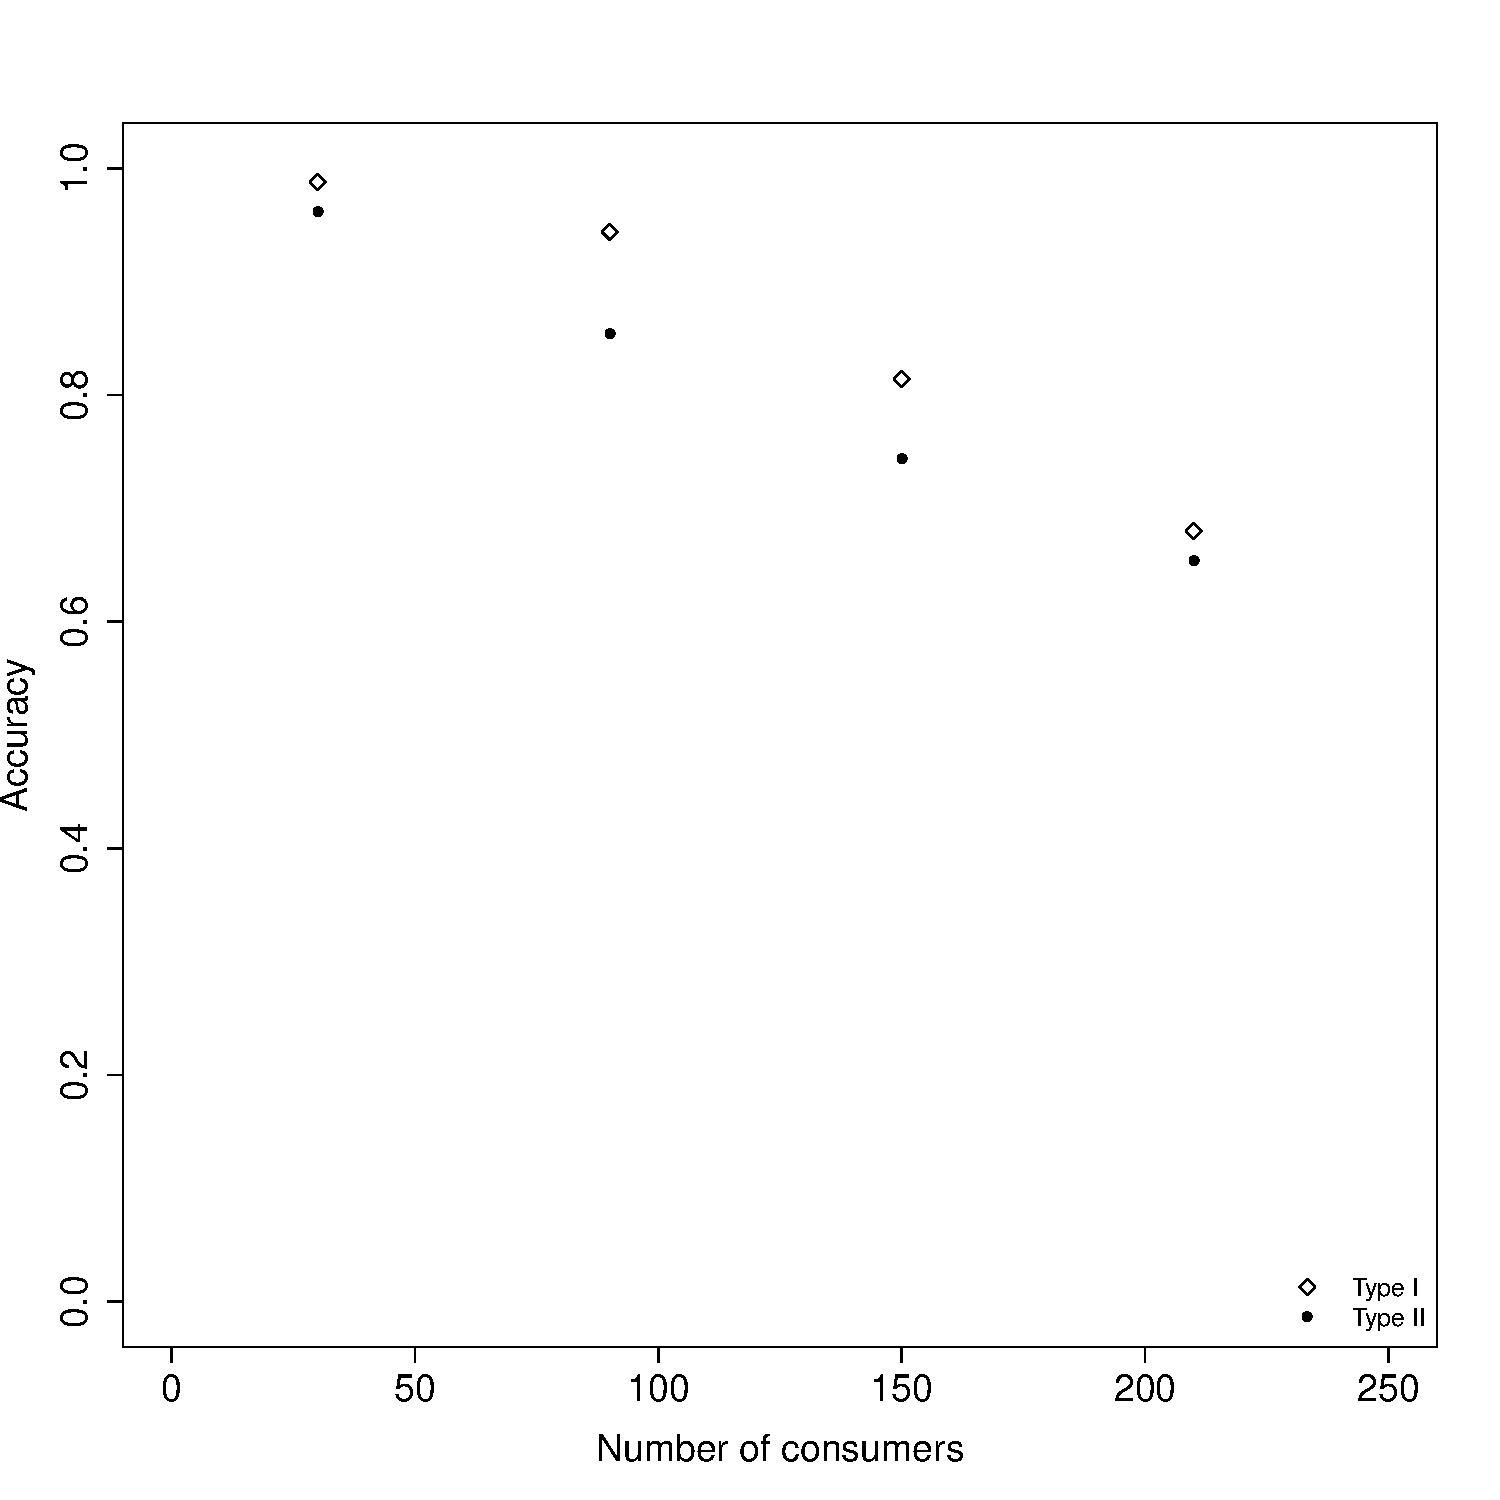
\includegraphics[scale=0.5]{../Images/Validation_exploitative.pdf}
 \caption{Accuracy (y-axis), expressed as the ratio of correctly predicted over actual extinctions, of the exploitative competition module over a range of $S_C$ values (x-axis). The base attack rates for the consumers used to test the module were sampled randomly from the range $10^{-6}-10^{-4}$. The number of resources is fixed at $S_R=300$. All other parameters are defined in Tab. \ref{tab:parameters}. Each point is calculated as the average of 500 replicates. Type I prediction are for when species should go extinct, type II for when both consumers can coexist.\label{fig:Validation_exploitative}}
\end{figure}


\subsection{Phyrric competition}
\label{sec:phy_comp}
The Phyrric competition module stems from  considering possible extinctions of resources driven by exploitative competition: consumer may compete so heavily for resources as to push the theoretical biomass of resources to below zero. Such a loss may cause further consumer extinction if it means they can no longer satisfy the invasibility criterion described by Eq. \eqref{eq:invadability_criterion}. Although a consumer may successfully outcompete another via this process, it is a Phyrric victory\footnote{A victory that bears such heavy costs to the victor that they also essentially loose. This term  dates to the \textit{Battle of Asculum} (279 BC), in which \textit{Pyrrhus of Epirus}'s victory over the Roman legions forced \texti{Epirus} to end his whole campaign due the heavy loss of casualties incurred.} given it has weakened itself in the process by loosing an important resource (as we will see below). To simplify this process I focus on the pair-wise competition between two consumer species $i$ and $j$ foraging on two resources and assume that
\begin{itemize}
\item Both consumers can overcome respiration according to Eq. \eqref{eq:invadability_criterion}
\item Neither consumer over-exploits either of the resources according to Eq. \eqref{eq:over_exploitation}
\item Neither consumer activates the serial extinction inequality given by Eq. \eqref{eq:serial_extinction}
\item Neither consumer out-competes the other according to the exploitative competition inequality Eq. \eqref{eq:exploitative}
\item Species $i$ and $j$ do not share their most important resource with one another. This can be written mathematically as $\max_k H_{k,i}\neq \max_k H_{k,j}$, where $\max_k H_{k,i}$ is species $i$'s strongest trophic link such that the trophic link $k$ satisfies $H_{k,i} > H_{l,i}$  $\forall l \neq k$
\end{itemize}
The condition for the resource corresponding to the trophic link $\max_k H_{ki}$ to go extinct using the above (calculated using Mathematica) is
\begin{equation}
H_{\text{max}_i,i} < H_{\text{max}_i,j}\label{eq:phyrric_b}
\end{equation}

i.e. if $i$'s strongest link is weaker than the strength of $j$'s equivalent link. I could not find a similar condition for the general case of  $S_R$ resources (the solution becomes intractable) so I proceeded to numerically estimate the accuracy of Eq. \eqref{eq:phyrric_b} for different values of $S_R$. Specifically I calculated how many times the most important resource of a consumer $j$ goes extinct when competing with another consumer $i$ over a range of resources $S_R$ by sampling the trophic links for both consumers using the parametrisation in Tab. \ref{tab:parameters}. The biomasses $B^*$ were calculated algebraically by solving the equilibrium condition of the resulting simplified food-web. To ensure that only the effect of consumer competition is captured, I set conditions such that none of the other extinction components (i.e. serial extinction, overexploitation, exploitative competition) are active during the examination of the final equilibrium solutions. The algorithm for this numeric validation is as follows:

\begin{enumerate}

\item Sample $S_R$ trophic links for a pseudo focal invader $i$ whose base attack rate is sampled from a range of base attack rates that resembles those found at equilibrium in the full model ($10^{-6}-10^{-4}$). Ensure that each respective pseudo resident can overcome respiration and then apply the serial extinction module to the initial trophic links. 

\item Sample a pseudo focal resident $j$ according to (1), if either pseudo invader or resident has more trophic links than the other, remove links at random such that both have the same number of trophic links. 

\item Ensure that both consumers can overcome respiration and that neither competes the other according to the exploitative competition module.

\item Ensure that $H_{\max_i,i}<H_{\max_i,j}$ and that $\max_i \neq \max_j$, i.e. that consumer $i$'s most important trophic link is smaller than the respective trophic link belonging to $j$, and that $i$ and $j$ do not share a common resource.

\item Calculate the equilibrium biomasses of $i$, $j$ and their shared resources algebraically, i.e. by only considering the system of two consumers and shared resources (rather than the whole food-web) according to Eq. \eqref{eq:LV_consumer1} and Eq. \eqref{eq:LV_resource1} and solving $B^*=A^{-1} r$. $M$ is the interaction matrix such that for $A={a_{ij}}$, $a_{ij}= - \epsilon a_{ji}$ and $a_{ii}=-\frac{s}{K}$   (intraspecific competition) for resources, else $a_{ii}=0$ for consumers. $r$ is the vector formed of elements $r_i$ that equal the respiration term $\rho$ for consumers, and the growth term $s$ for resources.

\item Record how many times $R_{\max_i}$, the most important resource of consumer $i$, goes extinct.

\end{enumerate}

I reproduced this algorithm over a range of $S_R$ resources as reported in Fig.~\ref{fig:Validation_phyrric} to show its accuracy (i.e. the proportion of correctly predicted extinctions) depends on the the number resources such that it increases with $S_R$. If we compare it to the range of $S_R$ experienced at quasi equilibrium, (roughly 200 - 500 number of species), this module achieves an accuracy between $50\%$ and $80\%$.

\begin{figure}[H]

\centering{}
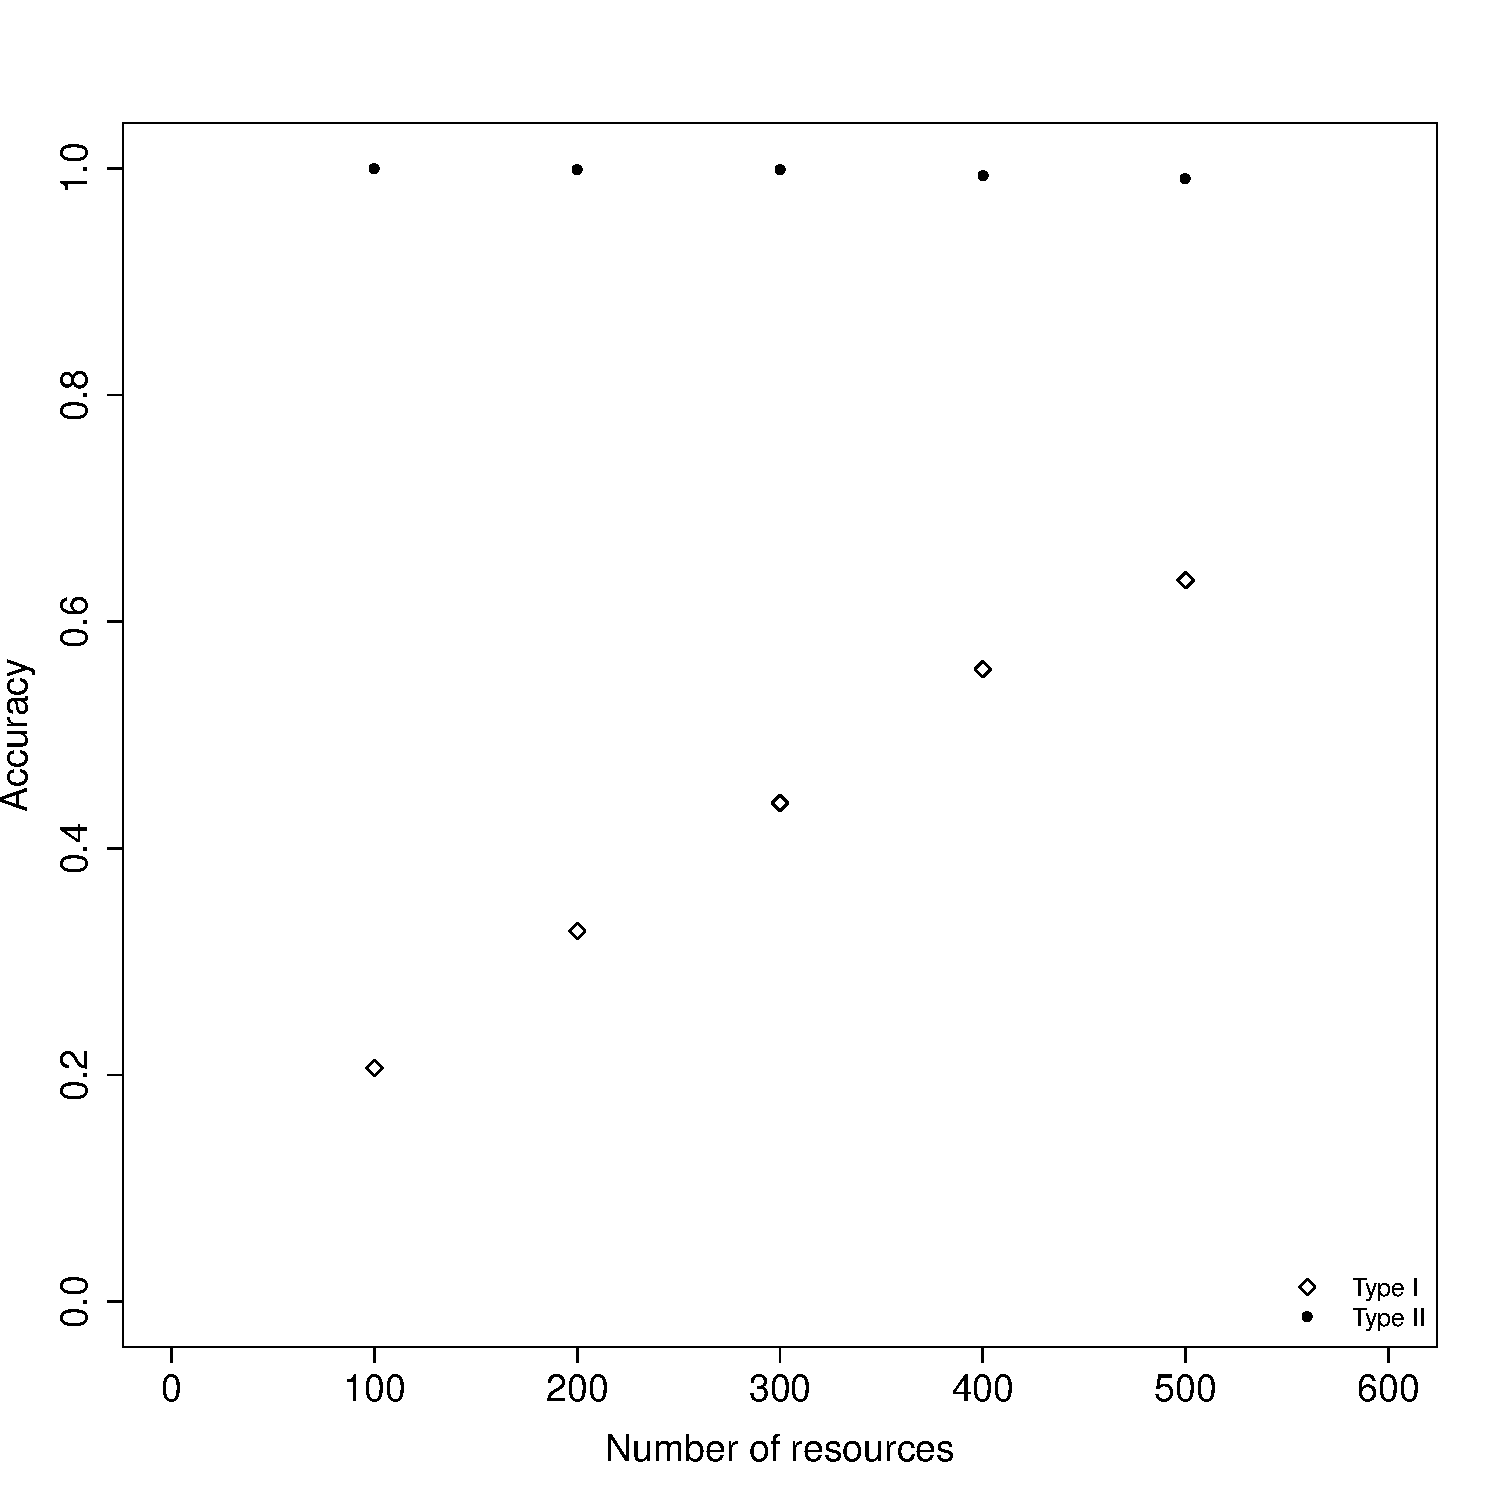
\includegraphics[scale=0.5]{../Images/Validation_phyrric.pdf}
  \caption{Accuracy (y-axis), expressed as the ratio of correctly predicted over actual extinctions, of the Phyrric competition module over a range of $S_R$ values (x-axis). The base attack rates for the consumers used to test the module were sampled randomly from the range $10^{-6}-10^{-4}$. All other parameters are defined in Tab. \ref{tab:parameters}. Accuracy of this module increases as the number of resources in the food-web system increases. Each point is calculated as the average of 500 replicates. Type I predictions are for when species should go extinct, type II for when both consumers can coexist.\label{fig:Validation_phyrric}}
\end{figure}


\subsection{Conclusion}

In this chapter I introduced a particular community assembly model studied by \citep{Rossberg2013} that forms the first part of a theoretical framework required to study the problem of overexploitation in consumer-resource systems. Whilst discussing the model's macroscopic behaviour, I highlighted the existence of an evolutionary steady state that is reached in Fig. \ref{fig:agg-through-time} during the evolutionary trajectory of community averaged base attack rates. This steady state suggests that types with intermediate attack rates are somehow evolutionary fittest, which is similar  to the emergence of "prudent predation" first envisioned by \citep{Slobodkin1968}: Predators that evolve to avoid overexploiting the very resources that they rely on for survival. Furthermore, the fact that this steady state is reached independently of the initial value of attack rates suggests some kind of constraint or negative feedback is shaping the evolutionary trajectory of attack rates. Given that no explicit constraints on attack rates are used in Eq. \eqref{eq:attack-rate-sampling}, this suggests that the constraint in the simulation is an intrinsic emergent property of the underlying food-web system. This emergence could potentially be similar to the trade-off associated with virulence that emerges from the co-evolution of parasites and hosts as suggested by \citep{Goodnight2008}. \\

Having discussed the difficulty in obtaining tractable expressions of steady state solutions for the community assembly model, which are necessary for inferring whether negative feedbacks associated with species type are indeed causing fitness trade-offs, I dedicated the rest of this chapter to constructing and validating the deconstructed assembly model and its individual components. This simplified variant of the community assembly model can now be used to study specific ecological processes within assemblages of consumer-resource food-webs. \\


The whole deconstructed assembly algorithm has been validated firstly by comparing the focal macroscopic characteristics we wish to study: the emergence of the time-series of food-web specific average base attack rate, and the associated average species richness, such that they both reaches a steady-sate fluctuating around a constant mean. That these phenomena appeared without any explicit constraints is essential, given the trade-off I wish to study is an emergent property of the full community assembly model and also appears without the need to specify any associated explicit constraints. For the full model, although this phenomenon of evolutionary stabilisation of base attack rates is known \cite[Fig.~20.8]{Rossberg2013}, the
underlying mechanisms have yet to be determined and discussed. I will show in the next chapter the main advantage of the deconstructed model is its ability to elucidate this opaque emergent phenomena and indeed interpret it in an ecological settings. \\

I argue that the use of the deconstructed model is a suitable simplification of the full model and that the disadvantages incurred are shadowed by its advantages. The main disadvantage of the deconstructed model is that of precision. The accuracy of the Phyrric and Exploitative competition modules vary according to the environment for example. Other modules such as serial extinction and invasibility criterion perform well and accurately depict and predict the ecological behaviour of the full assembly model. In terms of the invasibility criterion, Fig.~\ref{fig:birth_prob} depicts how this approximation improves if we apply a correction $\alpha$ to $K$. This is achieved in order to reflect the effect that other consumers residents have on  the biomass of resident resources. In the next chapter I show how we can improve this approximation further by taking in to consideration the effect that resident consumers have on the potential invaders. The main advantage is that given the macroscopic features of the full model we wish to study are recreated using the deconstructed model, one can now use this model to infer meaningful ecological and evolutionary mechanisms from it. The serial extinction module is a good example of this given that it clearly and accurately depicts a negative feedback occurring according to species types: Species with higher attack rates will incur stronger negative feedbacks in the form of the loss of important resources. \\

 As we will see in the next chapter, persistence of the system depends on the interaction of evolutionary forces represented by $\gamma_0$, the mutation bias parameter\footnote{This parameter controls deleterious effects that result from the accumulation of mutations at loci not under strong selection.}, with a trade-off that can be mechanistically explained with the deconstructed assembly model. Finally, I argue that the methodology underlying the deconstructed model, i.e. that of simplifying and breaking down the numerical integration of complex dynamical systems, may well transcend the original objective of this thesis. It has the potential to serve other studies that implement coupled non-linear differential equations to study food-web communities and which face similar problems of intractability. I can therefore focus on using only the deconstructed model from now on to study the problem of overexploitation, and only require the full assembly model for further validation processes. \\
  
\chapter{Ecological mechanisms constraining attack rates via the "live-fast die-young" trade-off \label{ch:chapter_3}}

\section{Introduction}

In this chapter I will demonstrate how studying the deconstructed variant of the predator-prey full community assembly model allows us to analyse a trade-off occurring between invasive ability and persistence. I will then mechanistically explain how this "live-fast die-young" trade-off constrains attack rates, such that a steady-state (first studied in \citep{Rossberg2008}) appears in their evolutionary trajectory. \\

The simulations by \citep{Goodnight2008} suggest that the evolutionary outcome of host-parasite metacommunity co-evolutionary models can be interpreted analogously in consumer-resource models. Specifically, the negative feedback associated with virulence - which affects the persistence of types and is incurred by the damage to the surrounding environment that parasites depend on - may occur analogously for the evolution of attack rates. In these simulations intermediate values of virulence are fittest, because they strike a balance between invasion fitness and persistence, such that long-term fitness is maximised. The authors argue that to study this phenomenon one must adopt a metacommunity focus and forgo mean-field approaches\footnote{An approximation of dynamical systems that compartmentalises the whole system. Each component is assumed to be identical on average. The study of the whole system can then be approximately studied by focusing on only one of these components}. The difficulty with using this metacommunity type setup to study whether analogous negative feedbacks occur in specific consumer-resource models are twofold and stem from the necessity of having to study many connected assembling food-web. First comes the issue of computational memory required to simulate a multi-patch community assembly model which is not impossible but significantly demanding. Then comes the problem of intractability of finding equilibrium solutions of dynamical systems composed of many coupled non-linear differential equations. These are necessary for elucidating the different facets that compose the fitness of consumer types.\\

I partially circumvented these hurdles by focusing on a evolutionary community assembly model first studied by \citep{Rossberg2013} (the second critical computational experiment that has inspired this thesis) that simplifies the multi-patch environment via a specific sampling paradigm: A single food-web assembly model that simplifies a metacommunity by imagining it is surrounded by other patches. The exchange of species makes all patches similar on average such that sampling species from within the patch approximates that of sampling from surrounding ones. The steady state that is reached during the evolutionary trajectory of attack rates, depicted in Fig. \ref{fig:agg-through-time}, clearly implies that some kind of constraint on attack rates exists. Moreover, given that an explicit constraint is not expressed in the model, this further implies that any constraint that exists is emergent. The possibility of an emergent constraint bolsters the possibility that the trade-off between invasive fitness and persistence, as alluded to by \citep{Goodnight2008}, is the most active in constraining attack rates. In this chapter I will firstly quantitatively prove this trade-off exists and will further understand it mechanistically. \\

The model studied in chapter 2 assumes that trophic traits evolve comparatively fast, such that the trophic niche of species are sampled completely randomly. One cannot affirm therefore, regardless of any mechanistic derivation, whether any resulting constraint studied in this chapter  would be robust to the advent of migration between patches in which this assumption is relaxed, i.e. one in which trophic niche information is retained. As I will explain in chapter \ref{ch:chapter_4} this leads to the problem of cheaters that is not explicitly treated in either the full or deconstructed assembly model. As a solution I propose to test any mechanisms that is derived from the community assembly model of \citep{Rossberg2008} in a simplified metacommunity simulation similar to that of \citep{Goodnight2008}.

 \section{Analysis of the Deconstructed Community Assembly Model}

In this section I will identify a mechanism for explaining how a negative feedback relative to the base attack rate leads to the emergence of a trade-off between short-term and long-term fitness, i.e. between invasive/dispersal ability and persistence. To achieve this, I mathematically decompose the long-term fitness, which is composed of invasion fitness and persistence. Specifically, for an existing population in a given patch, I measure how many new populations in other patches it may generate on average. To incorporate the effect of the mutation bias into the long-term fitness of types I will use the Price equation, which I introduce in the next subsection. I will then relate how the base attack rates $a_i$ of consumer populations affect their fitness.

\subsection{Evolutionary forces}
\label{sec:evolutionary-forces}

The first step required to disentangle the evolutionary forces that allow the stabilisation of base attack rates, is the construction of the relevant fitness landscape. I therefore re-iterate the perspective one must adopt when tackling the problem of overexploitation. According to \citep{Goodnight2008} one must account for the contrasting effects of invasion fitness and persistence. Invasion fitness is reported as the initial invasive and/or dispersal ability, and is the simplest component given it can be measured from a single individual and quantifies the relative immediate advantages of one type over others. Persistence describes the ability with which a type can survive and further reproduce once it has affected the environment and thus generated feedbacks. This is a more complicated measure because it must encapsulate the effects of any feedbacks in the environment that result from an invasion, thus they can only be inferred after invasion. This component of fitness therefore no longer stems from a single individual, but rather from the effect of a particular type of individual establishing itself in a population and/or geographic location. The first fitness component must quantify the invasive ability of a single individual. This is the ability to satisfy the invasibility criterion defined in Eq. \eqref{eq:invadability_criterion}, which is given by $\sum_{k=1} H_{ki} -1 $, i.e. the weighted sum of trophic links of a species $i$. The second fitness component includes the persistence of that individual's type once it has established and spread through out the species.\\

The unit of selection initially occurs at the individual level, i.e. at the point of invasion when only a handful of mutants are assumed to attempt an invasion. To correctly incorporate the facets of fitness, types have to be characterised at the species level. I then assume that as the species grows in density, all the traits belonging to the individuals within it are identical to those that initially entered and established that patch. To
bring our model for inheritance of base attack rates,
Eq. \eqref{eq:mutation}, into a mathematically more suitable form, I
express it in terms of logarithmic base attack rates:
\begin{equation}
  \log_{10}(a_{i})=\log_{10}(a_r) + \log_{10}(\gamma_{0}) + {\xi} \log_{10}( \gamma_{1}).\label{eq:log-mutation}
\end{equation}

In Figs.~\ref{fig:fitness-decomposition} (a) and (e) I show that
$\log_{10}(a)$ is approximately normally distributed in the steady state of
both the full and the deconstructed model, suggesting that a representation of the fitness landscape in term of $\ln(a_i)$ is more suitable for mathematical analysis than one in terms of $a_i$. Given $\xi$ is the only random variable (distributed as a standard normal), it is clear that $\log_{10}(\gamma_{0}$) represents the
size of the mutation bias for $\log_{10}(a_i)$, and $\log_{10}(\gamma_{1})^2$ the mutational
variance. \\

\subsection{The Price equation}

The effect of mutation bias on trait evolution is best understood at
the level of the Price equation \citep{Price72:_ExtensionCovariance},
which I interpret here by applying the unifying formulation of
evolutionary dynamics of \citep{Page2002}. In it the
expected rate of evolutionary change of the trait $q$ is given by
\begin{align}
  \label{eq:price}
  d \mathsf{E} q/dt = \cov[f(q),q] + \mathsf{E} \dot q,
\end{align}

with $f(q)$ denoting the invasion fitness of species of type $q$ and
the last term representing the mutation bias (the mean inherent rate
of change of traits). We are looking for trait values $q^*$ where the
left-hand-side, and hence the right-hand-side, of Eq. \eqref{eq:price}
evaluate to zero, so-called evolutionary singular strategies.
Following \citep{Page2002}, I expand $f(q)$ to first order at $q=q^*$, which approximates to $ \cov[f(q),q] \approx f'(q^*)\var q$, re-substituting this into Eq. \eqref{eq:price} then yields

\begin{align}
  \label{eq:price2}
  d \mathsf{E} q/dt = f'(q^*)\var q + \mathsf{E} \dot q,
\end{align}

The population-dynamical equilibrium condition implies that left hand side of Eq. \eqref{eq:price2} equals zero during the stead-state or equivalently

\begin{align}
  \label{eq:ess}
  f'(q^*) = - \frac{\mathsf{E} \dot q}{\var q}.
\end{align}

This condition generalizes the conventional criterion for evolutionary
singular strategies, that $f'(q^*)=0$, to situations with mutation bias. To continue we need to define and determine $f(q)$, i.e. the fitness as functions of species type, $q$. \\

\subsection{Defining and validating fitness}

I proceed by setting the trait parameter $q$ in the Price equation as being $\log_{10}(a_i)$ (I use a logarithmic transformation of $a_i$ because it is log-normally distributed). All that is left is do define $f(\log_{10}(a_i))$, i.e. the fitness of types. In a review by \citep{Metz}, one of the most relevant measure of fitness is given as the  mean of lifetime reproductive success, which is the average number of offspring that reach reproductive age during the lifetime of an individual, which I denote by $R(\log_{10}(a_i))$. The unit corresponding to offspring in this simulation is a mutant attempting to invade a web. Reproductive age is therefore analogous to successfully invading the food-web, and lifetime is the time spent (measured in consumer additions) in the food-web before going extinct. The birth and death rates typically associated with individuals become analogies for the birth and death rates of populations. Our measure of fitness for a resident $i$ therefore becomes the total number of mutants derived from $i$, that successfully invaded during its lifetime. Next, consider that in both the full and the
deconstructed model the ancestors of potential mutant consumer invaders are chosen at random with equal probability from the pool of
resident consumers. Then the probability that a given species gives rise to
a new invasion is independent of the lifetime of that species. This independence allows the factorisation of mean lifetime reproductive success. Specifically, $R(\log_{10}(a_i))$ (equivalent to $f(q)$ in the Price equation) 
becomes the product of the mean rate $b(\log_{10}(a))$ at which species generate
new invaders---their ``birth rate''---and the mean lifetime of
species: $R(\log_{10}(a)) = b(\log_{10}(a))L(\log_{10}(a))$ and hence

\begin{align}
  \label{eq:R-factorise}
  \log_{10}\{R[\log_{10}( a)]\} &= \log_{10}\{b[\log_{10}(a)]L[\log_{10}(a)]\}.
\end{align}

Validation of this decomposition is given in Figs.~\ref{fig:fitness-decomposition}: In (b) and (f) where I show how the average fitness of types (black curve) is accurately estimated using Eq. \eqref{eq:R-factorise} (dotted red curves) for both model types. Finally, validation of Eq. \eqref{eq:R-factorise} is achieved by applying Eq. \eqref{eq:ess} to the community assembly model: I set $q=\log_{10}(a_k)$ and
$\mathsf{E} \dot q= \frac{\log_{10}( \gamma_0)}{L^*}$, where $L^*$ is the mean
lifetime of populations in the community at equilibrium.  I determined
$\var q=\var \log_{10}(a)$ from the distribution of $a$ over the simulation
steady state. The steady-state invasion fitness, i.e. the mean inherent
rate of increase ($f(q)>0$) or decrease ($f(q)<0$) of the number of
populations of type $q$ in the simulation steady state, was approximated as
$f(q)\approx \log_{10}[R(\log_{10}(a))]/L(\log_{10}(a))$. Here $R(\log_{10}(a))$ is the the fitness of types $\log_{10}(a)$ 
of populations that inherit their base attack rate \emph{via}
Eq. \eqref{eq:mutation} from a population with base attack rate $a$. $L(a)$ is the mean
lifetime of populations with base attack rate $a$.  With $a^*$
representing the geometric mean of $a$ over the simulation steady
state, such that $\log_{10}(a^*)$ is the arithmetic mean of $\log_{10}(a)$, I expect
that $R(a^*)=1$. This in turn should lead to
\begin{align}
  \label{eq:fprime}
  f'(q^*)\approx\left.
  \frac{d[R(\log_{10}(
  a))]/L(\log_{10}(a))}{d\log_{10}(a)}
  \right|_{a=a^*}=
  \left.
  \frac{1}{L(\log_{10}(a))}\frac{d\log_{10}[R(\log_{10}(a))]}{d\log_{10}(a)}
  \right|_{a=a^*}\approx
  \left \frac{1}{L^*}\frac{d\log_{10}[R(\log_{10}(a))]}{d\log_{10}(a)}\right|_{a=a^*}.
\end{align}
Eq. \eqref{eq:ess} can therefore be written as
\begin{align}
  \label{eq:ess-agg}
  \left.\frac{d\log_{10}(R(\log_{10}(
  a))]}{d\log_{10}(a)}\right|_{a=a^*} \approx -\frac{\log_{10}(\gamma_0)}{\var\log_{10}(a)}.
\end{align}
Verifying Eq. \eqref{eq:ess-agg} means our definition of fitness satisfied the Price equation in Eq. \eqref{eq:price} and is therefore suitable for studying the underlying evolutionary forces. I achieve this graphically in
Fig.~\ref{fig:fitness-decomposition}b and~f.  Specifically, I find,
as expected, for both the full and the deconstructed model (i) that
$\log_{10}(R(\log_{10}(a^*)))=0$, and (ii) that the straight line with slope
$-{\log_{10}(\gamma_0)}/{\var\log_{10}(a)}$ is tangential to the curve
$\log_{10}(R(\log_{10}(a)))$ at $a=a^*$. Furthermore, the mutation bias slope is tangential at the point equal to the average base attack rate at equilibrium, at which fitness is equal to zero. \\

These results confirm that $R(\log_{10}(a))$ can be used as a fitness proxy in the analysis of mechanisms driving the evolution of base attack rates in the community assembly model. We can now clearly see how the fitness of consumer species is defined by a trade-off. As base attack rates increase, so do birth rates (Figs.~\ref{fig:fitness-decomposition} (c) and (g)), but at the cost of decreasing lifetime spent in the food-web (Figs.~\ref{fig:fitness-decomposition} (d) and (h)). The birth rate component of fitness $\log_{10}(b(\log_{10}(a_i)))$ exhibits the increasing
trend with $a_i$. This confirms the naive expectation that larger base attack rates increase the likelihood of a consumer having access to sufficient amount of
resources needed to sustain its population. In fact this
curve can be understood at an analytic level. In
Figs.~\ref{fig:fitness-decomposition} (c) and (g) I included two analytic predictions for
$\log_{10}(b(\log_{10}(a_i)))$. The first (green solid line) is based on transformation of the
invasibility condition into a probability as explained in Sec.\ref{sec:inv}. The full calculation of the birth rate then takes into account the mutation bias and the fact that I measure time in units
of consumer invasions and is presented in Sec. \ref{sec:mech_det}. As is clear from
Figs.~\ref{fig:fitness-decomposition} (c) and (d), this prediction does not fit
the data well. The prediction in Sec. \ref{sec:deconstr-food-web} can be improved (green dashed line) by relaxing
the simplifying assumption that the invader does not compete with
other consumers for its resources. Much more surprising is the dependence of lifetimes $L(\log_{10}(a_i))$ on base
attack rates. On the basis
that high exploitation rates are beneficial for Phyrric and Exploitative competition (and so protect against extirpation) one would naibly expect to see an increase of $\log_{10}(L(\log_{10}(a_i)))$ with
$\log_{10}(a_i$). Instead I find a weak decline
of $L(\log_{10}(a_i))$ with $\log_{10}(a_i$). That is, the higher a consumer's base attack rate, the
shorter is the average time until its extirpation from a community
(see Fig.~\ref{fig:fitness-decomposition} (d) and (h)). \\

We can now build a clearer picture for how different evolutionary forces interact with one another in such a way to constrain the evolution of $a_i$. In the previous chapter I discussed how $\gamma_0$ has to be below a threshold value to achieve persistence. In Fig.~\ref{fig:fitness-decomposition} we see why given that for no mutations bias (such that $\gamma_0=1$ and $\log_{10}(\gamma_0)=0$), then the value of $\log_{10}(a_i)$ for which Eq. \eqref{eq:price2} will be zero is exactly the point at which $\log_{10}(R(\log_{10}(a_i)))$ becomes stationary. This does not occur in the observed range of base attack rates, and presumably does so for a value of base attack rates that results in the evolutionary domination of overexploitative types. I also discussed how $\gamma_0$ on average decreases the value of $\log_{10}(a_i))$ whilst increasing the number species during the steady state. This can be explained using Eq. \eqref{eq:price2} and Fig.~\ref{fig:fitness-decomposition}: Decreasing $\gamma_0$ is equivalent to making the mutation bias slope in Fig.~\ref{fig:fitness-decomposition} (b) and (f) steeper, thus lowering the point that it is tangential to $\log_{10}(R(\log_{10}(a_i)))$. For persistence to be achieved, such that $\log_{10}(a_i)$ values do not evolve beyond to a threshold that leads to overexploitation, $\log_{10}(R(\log_{10}(a_i)))$, $\gamma_0$ and $\text{var}\log_{10}(a_i)$ have to interact in such a way that Eq \eqref{eq:price2} is satisfied below this threshold value. It is crucial therefore that $L(\log_{10}(a_i))$ decreases as a function of $a_i$, if it did not Fig. \ref{fig:fitness-decomposition} tells us that  the resulting fitness curve $\log_{10}(R(\log_{10}(a_i)))$, which equals the sum of $\log_{10}(b(\log_{10}(a_i)))$ and $\log_{10}(L(\log_{10}(a_i)))$, in agreement with Eq. \eqref{eq:R-factorise}, would no longer slowly saturate. Indeed, if lifetime were to increase with $a_i$ (as one would naively expect) then so should $\log_{10}(R(\log_{10}(a_i)))$. In this scenario the mutation bias would therefore have to be much stronger to achieve persistence. To understand the live-fast die-young trade-off between birth rates and lifetime as functions of $a_i$ I continue by mechanistically decomposing these in the following subsections. \\

% Graph created in final_paper_graphs_2.R
\begin{figure}[H]
  
\begin{center}
  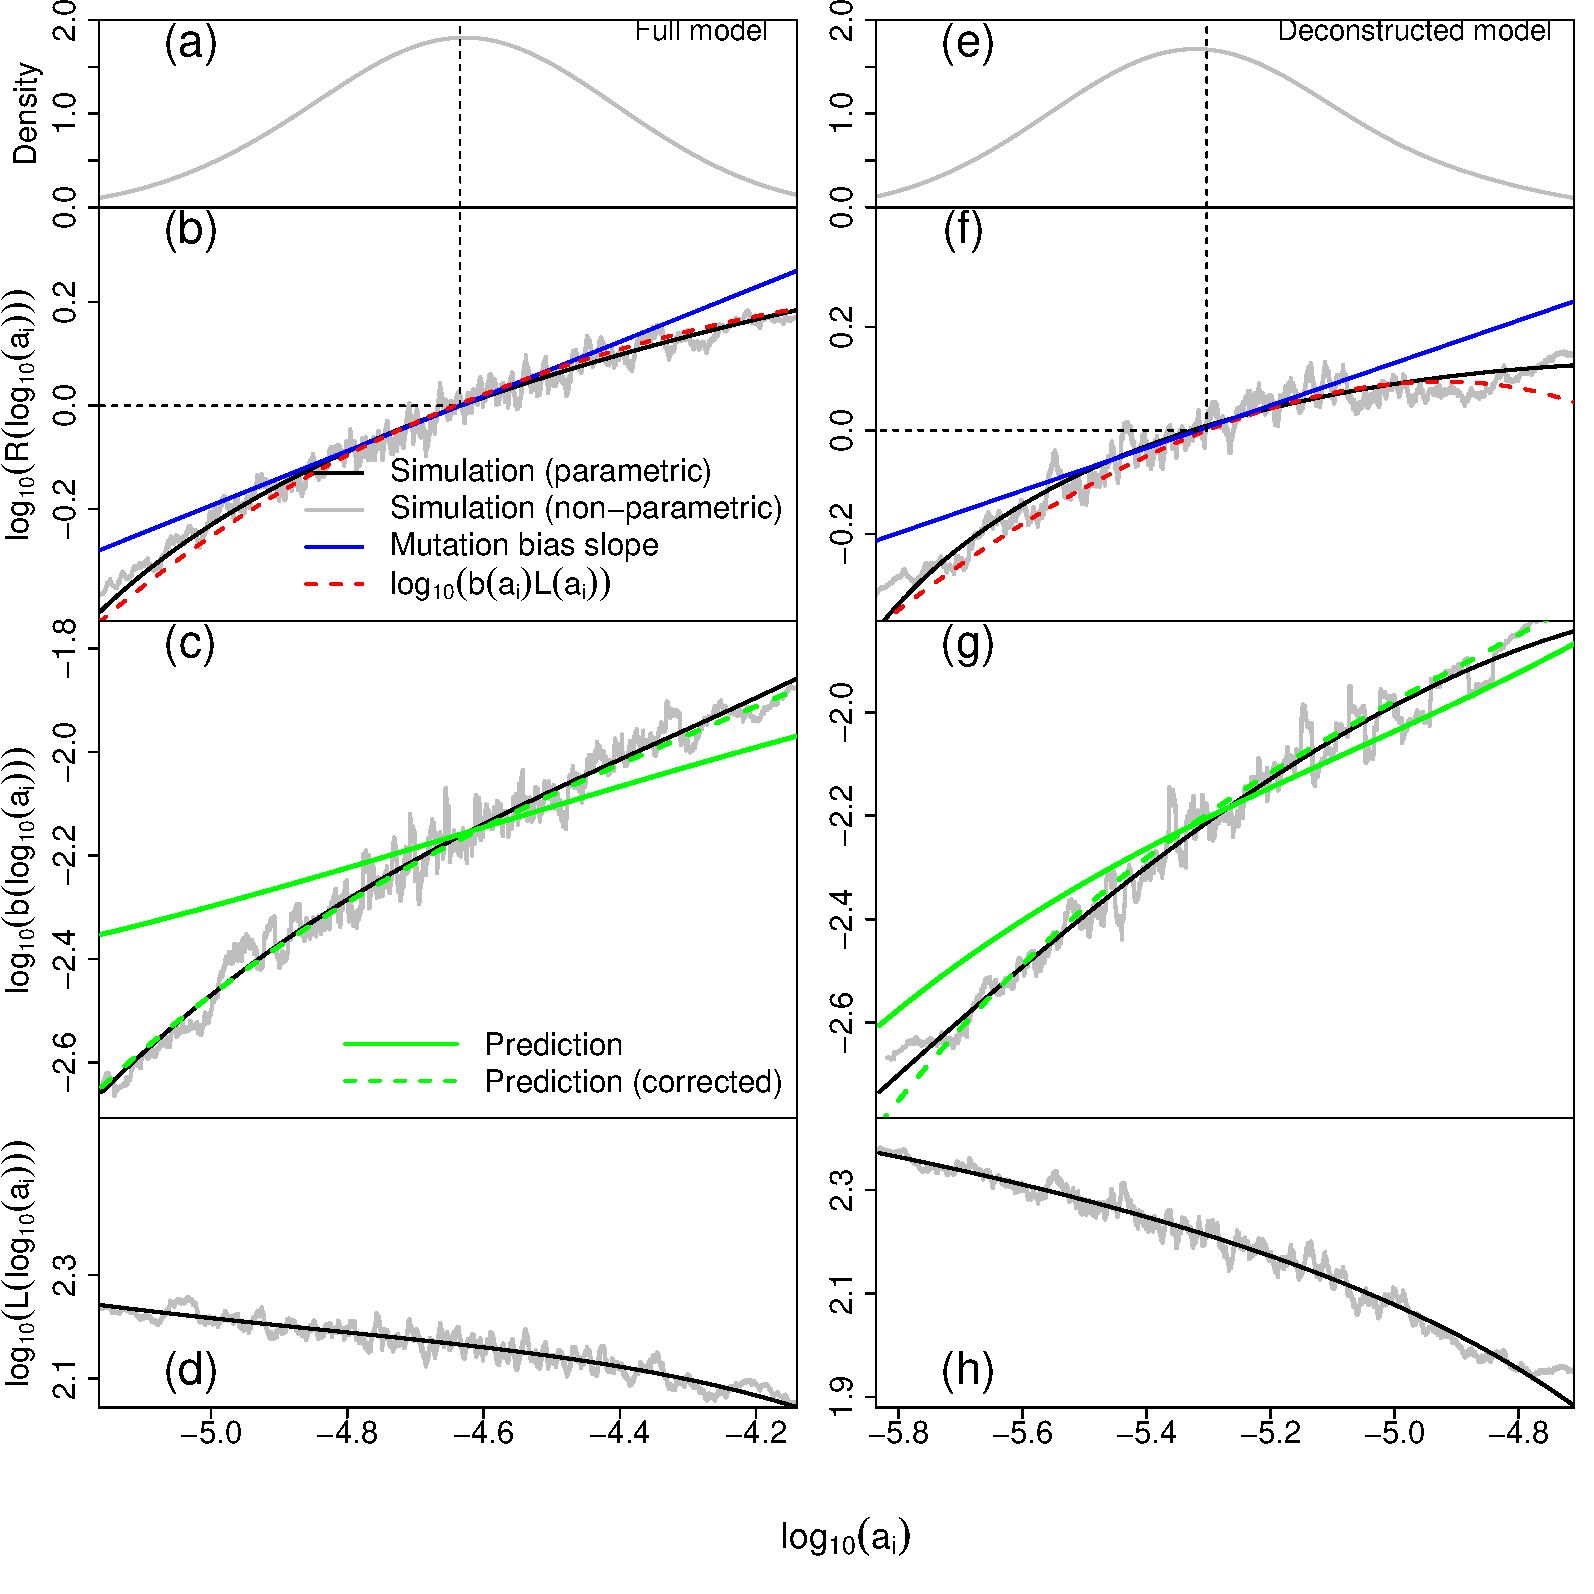
\includegraphics[scale=0.6]{../Images/All_deconstructed.pdf}
\end{center}
\caption{Panels (a) and (e) represent the distribution of $\log_{10}(a_i)$ values at quasi-equilibrium, the mean of (a) and (e) correspond to fittest values of $\log_{10}(a_i)$ (on average) in the simulation. The mean of (a) and (e) should correspond to the point where the fitness function in boxes (b) and (f), depicted by the black (rolling mean average) and grey (parametric fit) lines, is tangential to the random drift due to mutational genetic degradation, i.e. the mutation bias slope depicted by the blue line. This correspondence is shown by drawing a dotted line from the maximum of the distribution of $\log_{10}(a_i)$ in (a) and (e) (the mean at equilibrium) to the point where the mutation bias slope is tangential with the fitness curve in (b) and (e). Furthermore this point should have fitness equal to zero, depicted by the horizontal dotted line. The bottom two rows show the decomposition of fitness into birth rate (boxes (c) and (g)) and lifetime $\log_{10}(L(\log_{10}(a_i))$  (boxes (d) and (h), and thus graphically display the "live-fast die-young trade-off": As $a_i$ increases, the ability to produce successful mutant types increases at the cost of decreased lifetime of the population spent in the food-web (i.e. decreased propagule persistence).   \label{fig:fitness-decomposition}
  }
\end{figure}\\

All curves in Fig. \ref{fig:fitness-decomposition} are generated using data taken during the steady-state of both assembly models, i.e. after $0.5 \times^5$ consumers were added. In panels (a) and (e) I estimate the density distribution of $\log_{10}(a_i)$ which are obtained using the “density” function available for R statistical software. The non-parametric curves in (b), (c), (d), (f), (g) and (h) are obtained using rolling mean function “rollmean” in the “zoo” package  available for R, using window sizes of 1000 for both x and y axis values. The parametric curves are calculated by fitting cubic functions over the non-parametric curves using the maximum likelihood curve fitting function "nls" also available for R. The predicted curves for the birth rates $\log_{10}(b(\log_{10}(a_i))$ in (c) and (g) are calculated according to Eq. \eqref{eq:birth_rate_final}. The (correction) annotation refers to the relaxation of the assumptions described in Sec. \ref{sec:mech_det} that leads to Eq. \eqref{eq:birth3_full_corrected} being used in Eq. \eqref{eq:birth_rate_final}. The mutation bias curve is calculated from the mutation bias slope in Eq. $\eqref{eq:mutation}$, $\gamma_0$,  by multiplying it by $\log_{10}(a_i)$. 

\subsection{Mechanisms determining $b(a)$ \label{sec:mech_det}}

To derive the birth rate $b(a_{r})$ of a resident of type $a_{r}$ we must mathematically express 
the various steps that form the invasion process in the Deconstructed Assembly algorithm i.e.

\begin{enumerate}
\item Selection of the resident $a_{r}$ over all others (given it is present in the food-web)
\item Sampling a random mutant $a_{m}$ from a resident according to Eq. \eqref{eq:attack-rate-sampling}
\item Attempt an invasion with the sampled mutant
\item If 3. fails, repeat from 1. until successful
\end{enumerate}

Steps 2 and 3 represent the probability $b(a \in \Re|a_{r})$ that
a resident $a_{r}$ \textbf{once chosen} will generate any invasively
fit mutant (i.e. for any value of $a\in\Re$). To account for
steps 1 and 4 and thus calculate \textbf{$b(a_{r})$} the probability
that $a_{r}$ is chosen \textbf{AND} generates any fit mutant offspring
we must consider that we ''force'' a mutant to invade at a particular
time-step and should therefore have that $\sum_{r\in S_{C}}b(a_{r})=1$
for that time-step. This implies that by summing $b(a_{r})$ over all consumer residents
in the food-web, this must add to one, which is satisfied for: 
\begin{equation}
b(a_{r})=\frac{b(a\in\Re|a_{r})}{\sum_{l=1}^{S_C}b(a\in\Re|a_{l})} \label{eq:birth_rate_final}
\end{equation}

 To establish the birth rate, I must first capture the distribution of the invasion probability. In chapter 2 I compared how the invasibility criterion can approximate the ability for a consumer to successfully invade by showing how the numeric estimate of successful invasion attempts of simulated food-webs qualitatively matches invasion attempts defined by Eq. \eqref{eq:invadability_criterion}. I also displayed its resemblance with the cumulative distribution function of a normal distribution (see Fig.\ref{fig:birth_verification}). To continue, I firstly note that the $\sum_{k=1}^{S_{R}}e^{\sigma\xi_{ki}}$ term is the sum of $S_R$ log-normal distributed random variables $e^{\sigma\xi_{ki}$ and is therefore itself also a random variable. I can subsequently approximate Eq. \eqref{eq:invadability_criterion} into an analytic probability distribution
\begin{equation}
P\Bigg[\sum_{k=1}^{S_{R}} \epsilon a_m e^{\sigma\xi_{km}} K<\rho\Bigg]
\label{eq:birth_prob_first}
\end{equation}
and compare it to its  numerical estimate, i.e. the invasion probability.

\paragraph{Invasion probability of a mutant invader: analytic approximation} To derive the analytic approximation for the probability of invasion, I first write down the probability that Eq. \eqref{eq:birth_prob_first} is satisfied and then re-arrange this expression as follows:
\begin{equation}
P\Bigg[\sum_{k=1}^{S_{R}}e^{\sigma\xi_{km}}<\frac{K\epsilon a_{m}}{\rho}\Bigg]=P\Bigg[\sum_{k=1}^{S_{R}}e^{\sigma\xi_{km}}<\alpha_{m}\Bigg]
 \label{eq:birth}
\end{equation}
where the dimensionless parameter $\alpha_m=\frac{K \epsilon a_{m}}{\rho}$. To proceed I note that the distribution of $\sum_{k=1}^{S_{R}}e^{\sigma\xi_kjm}$ is analytically unknown, I thus use the approximation derived in \citep{Rossberg2011a} such that
\begin{equation}
P\Bigg[\sum_{k=1}^{S_{P}}e^{\sigma\xi_{km}}<x\Bigg]\approx\prod_{k=1}^{S_{R}}P\Bigg[e^{\sigma\xi_{km}}<x\Bigg]=\Phi\Big(\frac{\ln(x)}{\sigma}\Big){}^{S_{P}} \label{eq:birth2}
\end{equation}
where $\Phi$ is the cumulative distribution function of a standard normal random variable. As shown in \citep{Rossberg2011a} the mean and variance of the resulting distribution in Eq. \eqref{eq:birth2} can be approximated by $y_{0}=\sigma\sqrt{2\ln S_{R}}$ and $\sigma_{0}=\frac{\sigma^{2}}{\sqrt{\sigma^{2}+y_{0}^{2}}}$ respectively such that
\begin{equation}
P\Bigg[\sum_{k=1}^{S_{P}}e^{\sigma\xi_{km}}<x\Bigg]\approx\Phi\Big(\frac{\ln(x)-y_{0}}{\sigma_{0}}\Big) \label{eq:birth44}
\end{equation}
Substituting $\alpha_{m}^{-1}$ for $x$, the invasion probability
for a mutant $m$ with $S_{R}$ possible trophic interactions to overcome
respiration (the invasibility criterion) becomes
\begin{equation}
I(a_{m};y_{0},\sigma_{0})\approx1-\Phi\Bigg(\frac{\log_{e}(\alpha_{m}^{-1})-y_{0}}{\sigma_{0}}\Bigg) \label{eq:birth3}
\end{equation}
I also determine the mean $y_{E}$ and standard deviation $\sigma_{E}$ of $\ln\big(\sum_{k=1}^{S_{R}}e^{\sigma\xi_{km}}\big)$ from $10^4$ independent samples for a specific value of $S_{R}$. Finally, in addition to using $y_0$, $\sigma_0$ and $y_{E}$, $\sigma_{E}$,  I estimated $y_{S_{R}}$ and $\sigma_{S_{R}}$ using
the "optim" function in R, by minimising the sum of squared errors $\sum_{i\in R^{a_{m}}}(I(a_{i})$-$I(a_{i})_{e})^{2}$,
over the range $R^{S_{R}}$ of the number of resources reported in the assembly simulations. Thus for each $S_{R}\in R^{S_{R}}$
I obtained a pair of $y_{S_{R}}$ and $\sigma_{S_{R}}$ estimates
for $I(a_{m}; y_{S_{R}},\sigma_{S_{R}})$ such that 
\begin{equation}
I(a_{m};y_{S_{R}},\sigma_{S_{R}})\approx1-\Phi\Bigg(\frac{\log_{e}(\alpha_{m}^{-1})-y_{S_{R}}}{\sigma_{S_{R}}}\Bigg).\label{eq:birth3-2}
\end{equation}

represents the best possible prediction of the numeric invasion probability using the analytic form of Eq. \eqref{eq:birth44}. It therefore serves as a benchmark for other variations of mean and variance used to parametrise it. The qualitative validation for the general use of the invasibility criterion is again provided in Fig.~\ref{fig:birth_prob} by comparing their approximate values based on Eq. \eqref{eq:birth3} (red, yellow and green curves) to the respective accurate numeric estimates (blue curves) obtained for the full and deconstructed model. I focus on the deconstructed first (solid lines), where the predictions using optimised  parameters (green) (using the "optim" function in R) are the benchmark for the best possible fits that are obtainable using the form Eq. \eqref{eq:birth3}. Thus we can see that predictions using analytically obtained parametrisations of mean and standard deviation for Eq. \eqref{eq:birth3-2} are worse than the numerically derived parameters (green). Comparison of the predictions (green and red curves) to the estimated (blue curves) probabilities shows that Eq. \ref{fig:birth_prob} reproduces the invasion probability for the deconstructed model well. However, comparison of deconstructed (solid) and full (dashed) numeric estimates shows that we can only qualitatively reproduce the invasion probability emerging from the full model. This is due to the approximation of  resources biomasses in Eq. \eqref{eq:invadability_criterion} which are set to their carrying capacity instead of their actually value at equilibrium. To correct for this I  assume that the biomass of resources is well approximated by their mean at equilibrium, and set $B^R_k=\overline{(B^R_k)^*}$ in Eq. \eqref{eq:invadability_criterion_2}. This correction is still quantitatively not perfect however, given that I am omitting the effect of species competition on the equilibrium biomass of the invader. 

% Graph created in invasion_prob_test_2.R
\begin{figure}[H]
\centering{}
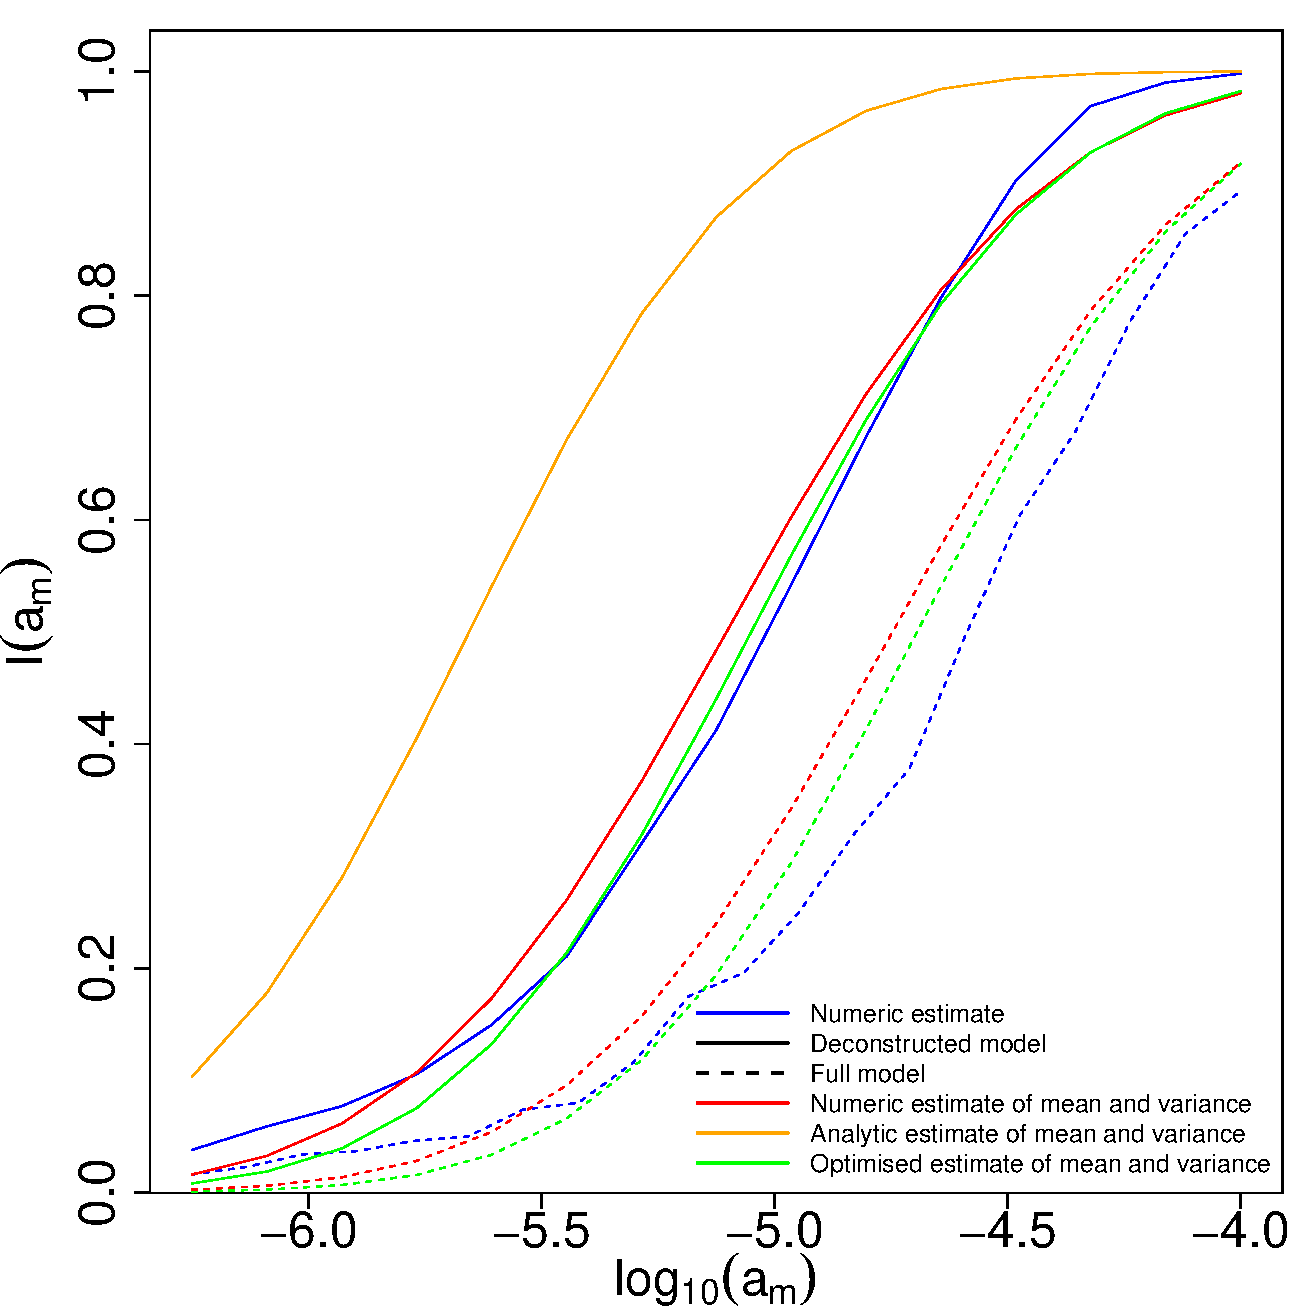
\includegraphics[scale=0.5]{../Images/Invasion_Probabillity.pdf}
 \caption{Invasion probabilities (y-axis) as functions of mutant's base attack rates $a_m$ (x-axis) attempting to invade a food-web with $S_R=300$ resources. The probabilities test the validity of Eq. \eqref{eq:invadability_criterion} by plotting the corresponding numeric (blue) and predicted (orange, red and green) invasion probabilities for 20 base attack rate values equally spaced logarithmically in the range spanning $10^{-6.25} - 10^{-4}$. Three distinct analytic probability distributions defined by Eq. \eqref{eq:birth3} are provided according to whether the underlying mean and variance parameters were approximated analytically (orange), numerically (red) or optimised (green). The solid and dashed lines respectively correspond to the Full and Deconstructed community models. All other parameters used to obtained these graphs are given in Tab. \ref{tab:parameters}. Each probability point calculated is an average over 500 replicates. 
\label{fig:birth_prob}}
\end{figure}

To continue, I note that $I(a_{m})$ is the probability of a mutant $a_{m}$ successfully invading once it is randomly
sampled from a resident $a_{r}$. This  can be used to construct $b(a\in\Re|a_{r})$ which I derive as being the expectation over all possible mutants being derived from a particular resident, times the probability they successfully invade. Next I identify the distribution that represents the sampling of log transformed base attack rates of mutants from a residents base attack rate $a_r$ according to Eq. \eqref{eq:attack-rate-sampling}, i.e. $\log_{10}(a_m)=\log_{10}(\gamma_0\gamma_1^{\xi}a_r)$. I firstly consider that $\xi$ is the only random variable. Therefore $\log_{10}(a_m)$ will also be normally distributed. Second I take into consideration the constants, i.e. the mutation bias, $\gamma_0$, and the variance surrounding the sampling of mutants, $\gamma_1$. The underlying mean of the normal distribution will therefore be equal to the expectation which equals $\log_{10}(\gamma_0a_r)$ and the variance will subsequently equal $\log_{10}(\gamma_1)^2$. The cumulative distribution function then becomes
\begin{equation}
\Phi\Big(\frac{\log(a_m)-\log(\gamma_0a_r)}{\log(\gamma_1)}\Big) \label{eq:mutant_prob}
\end{equation}
where $\Phi(x)$ represents the cumulative distribution function of a standard normal random variable. $b(a\in\Re|a_{r})$ will subsequently be the convolution of the probability of sampling a particular mutant $a_m$ from resident $a_r$ and the probability $I(a_{m})$ of that mutant successfully invading
\begin{equation}
b(a_{m}\in\Re|a_{r})=\int_{-\infty}^{\infty}I(a_m)\Phi\Big(\frac{\log(a_m)-\log(\gamma_0a_r)}{\log(\gamma_1)}\Big)da_m. \label{eq:birth_rate_final}
\end{equation}

To test the birth rate given by Eq. \eqref{eq:birth_rate_final} I ran a model containing the elements of the invasion algorithm of the deconstructed model for a fixed range of base attack rate values (the pseudo-residents). To successfully invade, a mutant had to a) overcome respiration and b) not be outcompeted by rival resident consumers that were obtained from a previously saved food-web. In Fig.~\ref{fig:birth_rate_comp} we compare the estimated birth rate of each pseudo resident against the predicted birth rate given by Eq. \eqref{eq:birth_rate_final} where the numerical and predicted rates are not well matched, I thus presumed that this was due to b). Indeed when I re-ran the experiment without the competition component (i.e invaders only have to overcome respiration) I obtain a good match between predicted and observed birth rates as shown in Fig.~\ref{fig:birth_rate_no_comp}. This confirms the effect that resident consumers have on the invaders ability to successfully establish themselves. \\

% Graph created in invasion_prob_test_2.R
\begin{figure}[H]
\caption{Comparison of the estimated (black) and predicted (red) birth rates  according to an invasion algorithm that samples pseudo invaders which will successfully invade if they a) overcome respiration and b) are not outcompeted by a rival resident consumer that were obtained from a previously saved food-web. \label{fig:birth_rate_comp}}
\centering{}
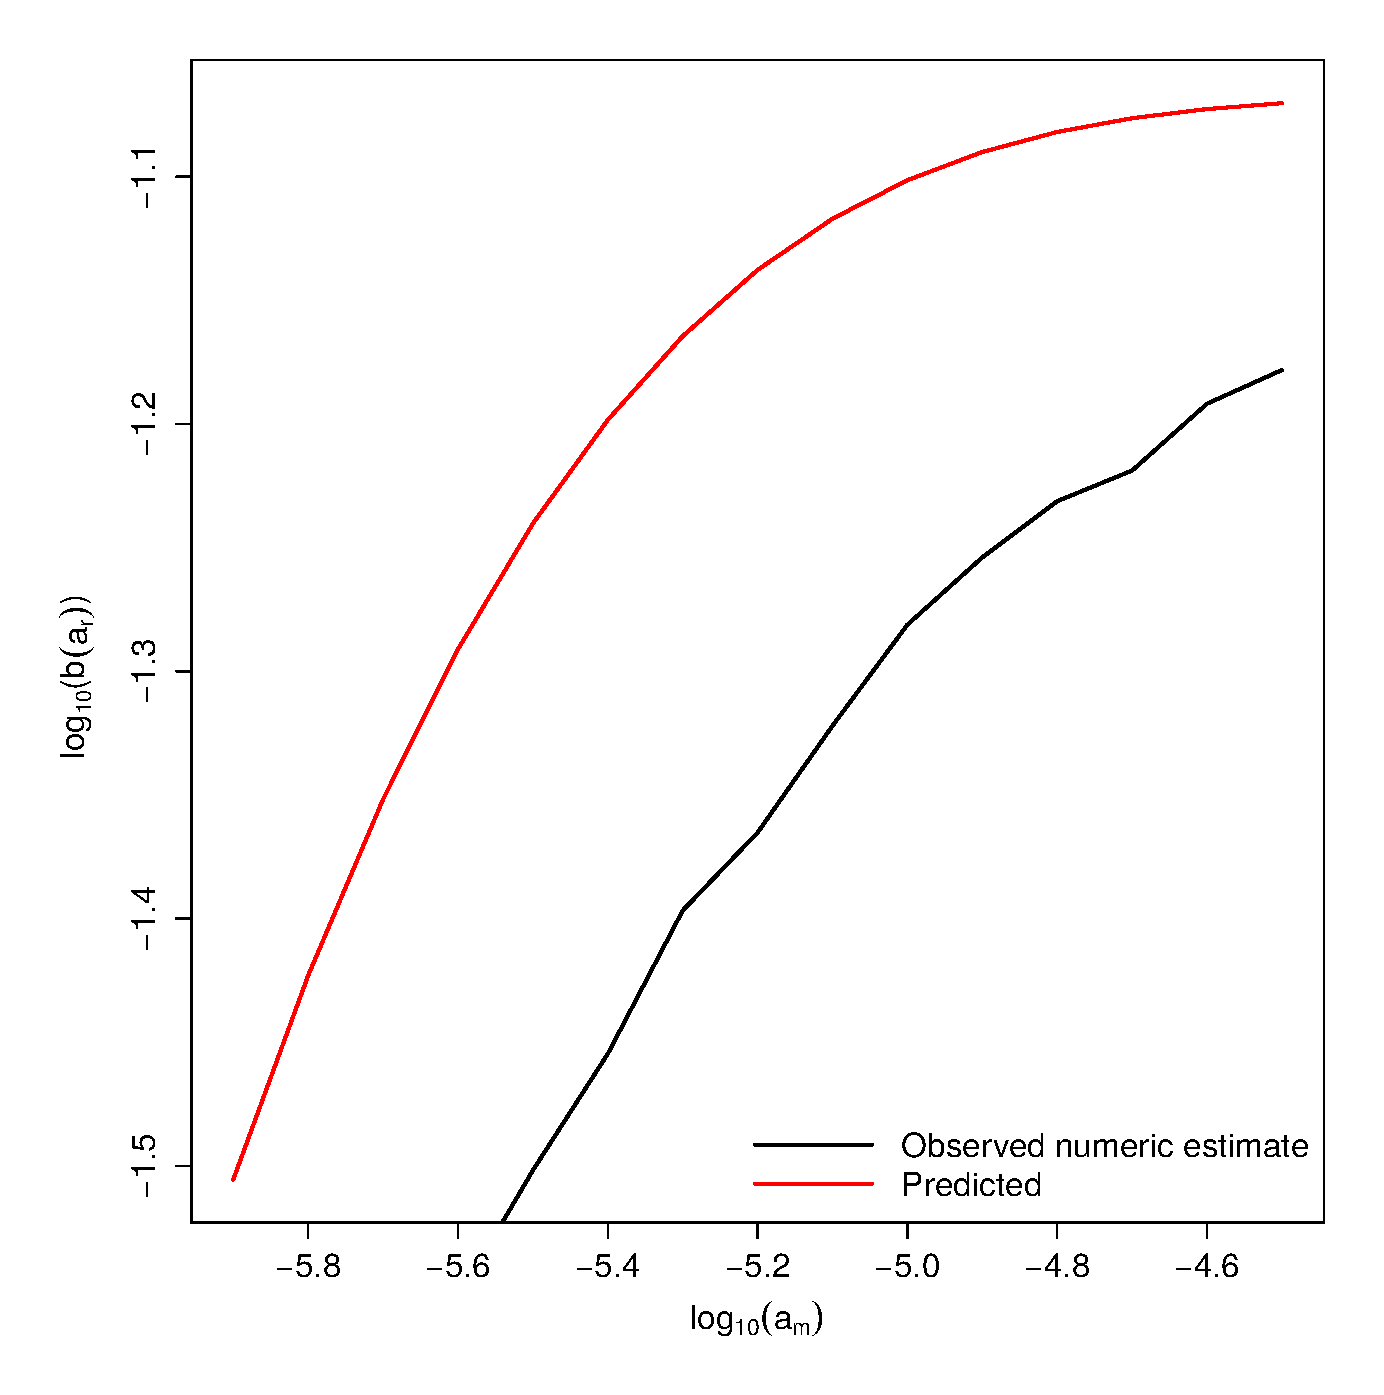
\includegraphics[scale=0.6]{../Images/Birth_rate_comp.pdf}
\end{figure}


% Graph created in invasion_prob_test_2.R
\begin{figure}[H]
\caption{Graph for comparing the estimated (black) and predicted (red) birth rates according to an invasion algorithm that sample pseudo invaders which will successfully invade if they they overcome respiration. \label{fig:birth_rate_no_comp}}
\centering{}
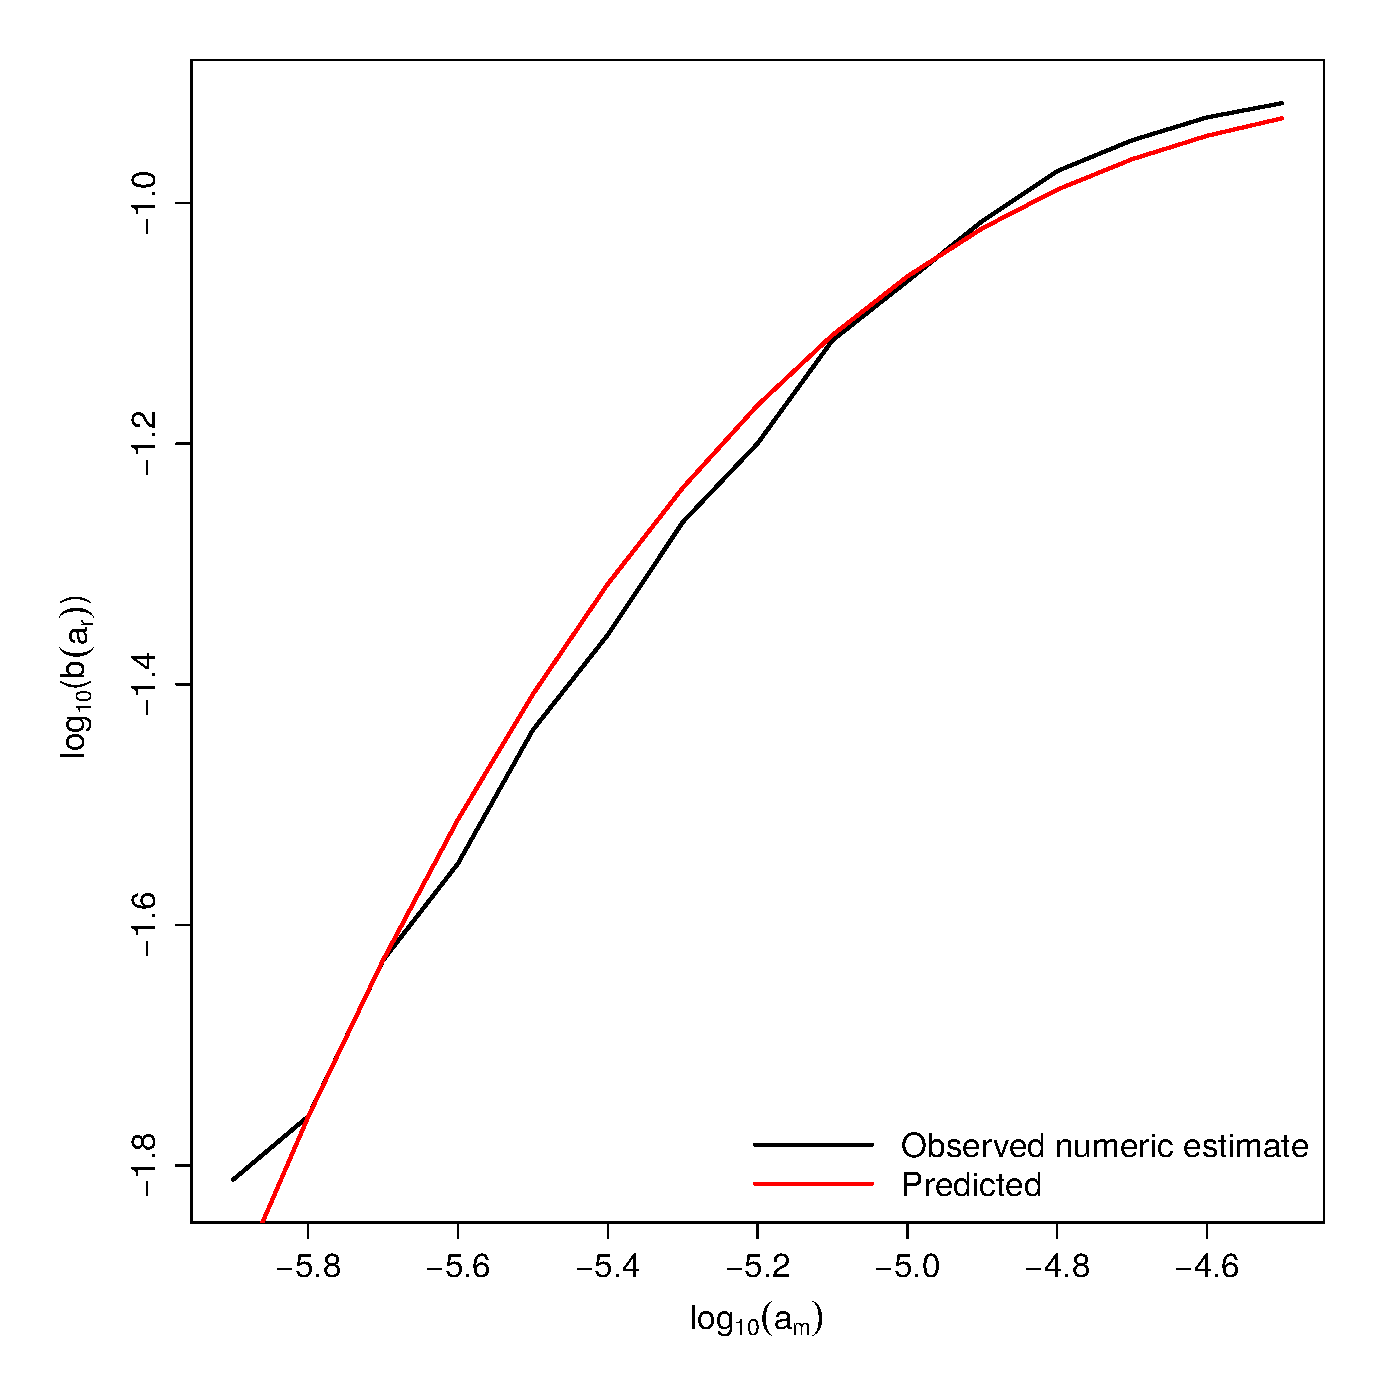
\includegraphics[scale=0.6]{../Images/Birth_rate_no_comp.pdf}
\end{figure}
 
  To consider the effect that resident consumers have on the the invader, I note that Eq. \eqref{eq:invadability_criterion} makes two critical simplifications that must be corrected. The first is that the transition from Eq. \eqref{eq:invadability_criterion_2} to Eq. \eqref{eq:birth_prob_first} for constructing the invasion probability Eq. \eqref{eq:prob_invasion} requires the approximation $B^R_k \approx K$ for all $k$. The second is that invasions are guaranteed as long as a consumer can overcome respiration. In terms of the latter we see that by rearranging the exploitative competition inequality in Eq. \eqref{eq:exploitative}, an invader's $i$ biomass will be positive if it can overcome competition from any resident $j$, i.e. if 
\begin{equation}
\min_j \sum H_{ki} [ 1 - H_{kj} (H_j-1)/(\sum_l H^2_{lj}) ] - 1 > 0. \label{eq:inv_crit_3}
\end{equation}
To continue note that the minimum (over all $k$ for given $j$) of the term contained within the square bracket of  Eq. \eqref{eq:inv_crit_3} is 
\begin{equation}
1 - \max_k H_{kj}(H_j-1)/(\sum_l H^2_{lj}) \label{eq:cor_fact}
\end{equation}
which is positive if and only if there is no more serial extinction, i.e. if
\begin{equation}
(\sum_l H^2_{lj}) > max_k H_{kj}(H_j-1).
\end{equation}

One can therefore expect that there are some $k$ for which Eq. \eqref{eq:cor_fact} is close to zero but positive. The factor  Eq. \eqref{eq:cor_fact} contained in Eq. \eqref{eq:inv_crit_3} is exactly the change in biomasses due to the presence of $j$ (assuming no other resident consumer has a sizeable effect). This factor takes values within the range 0 to 1. One can further expect, that for the consumer $j$ with the strongest overlap with $i$, the Eq. \eqref{eq:cor_fact} can be approximated by some constant correction factor $\beta$ well within the range 0 to 1.  \\

%%%%%%%%%%%%%%%%%%%%%%%%%%%%%%%

%\begin{equation}
%H_{i}>\sum_{k=1}H_{ki}H_{kj}\frac{(H_{j}-1)}{\sum_{k=1}H_{kj}^{2}}+1 \label{eq:inv_crit_2}
%\end{equation}
%
%in our current simplification of the invadabilty criterion, invasion is achieved if $H_{i}>1$, which omits the effects of consumer competition outlined in Eq. \eqref{eq:inv_crit_2} which have to be considered in both the full and deconstructed assembly model. The right handside of Eq. \eqref{eq:inv_crit_2} can thus be simplified via a term $\frac{1}{\beta_{ij}}$ such that the invadability criterion for the deconstructed model becomes
%
%\begin{equation}
%\sum^{Sr}_{k=1} H_{ki}B^R_j\beta_{ij}>1. \label{eq:inv_crit_3}
%\end{equation}
%
% For the full model we must further consider the effect of consumer competition on  $B^R_j$. The vector of equilibrium resource biomasses $B^R$ is shown in \citep{Rossberg2013} to be a function of consumer competition
%
%  
%\begin{equation}
%B^R = \Big(C^P\Big)^{-1} \Big[s^P - A^{'} \Big( \hat{C}^C \Big)^{-1}\hat{s} \Big] 
%\end{equation}  
%  
%   given it contains the bi-partite interaction matrix $A$ and the vector of equilibrium consumer biomasses $ \Big( \hat{C}^C \Big)^{-1}\hat{s} $, which as shown in section \ref{sec:exploitative_comp} is itself a function of consumer competition. Thus the effect of consumer competition on an invader can also be captured through the equilibrium biomasses of resource and therefore via our simplification of setting $B^R_j=K$ for all $j$ in Eq. \eqref{eq:prob}, which in its current form may be unsatisfactory given that it implies all resources exist at carrying capacity at equilibrium and are unaffected by multiple consumers. We again face the problem of intractability at this point when handling the equilibrium biomasses of an arbitrary number of consumers and resources. If we reduce the problem as per the exploitative competition modules, the equilibrium biomasses become a function of the exploitive competition inequality such that
%   
%\begin{equation}
%B^R_k = \frac{K_k}{r_k} \Big[g_k - A_{ki}b^C_i  - A_{kj}b^C_j \Big] = \theta_{k,i,j} \label{eq:simp_res_biom}
%\end{equation}  
%  
%Thus by joining the effects of competition on resource and invader biomasses according to Eq. \eqref{eq:simp_res_biom} and Eq. \eqref{eq:inv_crit_3} respectively, the invadability criterion for an invader $i$ in the full model becomes 
%
%\begin{equation}
%\sum^{Sr}_{k=1}H_{ki}\beta_{ij}\theta_{k,i,j}=\sum^{Sr}_{k=1}H_{ki}\theta^c_{k,i,j}>1. \label{eq:inv_crit_3}
%\end{equation}
%   
%where $\theta^c_{k,i,j}=\beta_{ij}\theta_{k,i,j}$. Instead of performing the birth rate predictions using exact calculations of $\theta_{k,i,j}$ and $\beta_{i,j}$ 

Instead of performing the birth rate predictions using exact calculations of $\beta$, I use an optimisation algorithm to obtain the value for a corrected version of Eq. \eqref{eq:birth3-2}. I firstly approximate the convolution in Eq. \eqref{eq:birth_rate_final} by a normal distribution, such that the probability of a resident yielding an invassively fit mutant is simply the invasion probability of that resident shifted by the mutation bias, where $\alpha_r_0=\alpha_r \times a_0$:
\begin{equation}
b(a_{m}\in\Re|a_{r})\approx I(a_{0}a_{r};y_{S_{R}},\sigma_{S_{R}})\approx1-\Phi\Bigg(\frac{\log_{e}(\alpha_{r_{0}}^{-1}\beta)-y_{S_{R}}}{\sigma_{S_{R}}}\Bigg)\label{eq:birth3_full_corrected}
\end{equation}

This assumes the approximation is valid for when the variance associated with the mutation, $\log_{10}(\gamma_1)^2\approx 3\times10^{-2}$ is much smaller than that of the invasion probability, which can be estimated as $\sigma_E$ defined in Sec. \ref{sec:inv} and which roughly equals 1.16). Then, for the full and deconstructed models, I generated optimised values of $\beta$ (respectively $\beta_F$ and $\beta_D$) of these by minimising the squared difference between the observed and predicted birth rates (respectively for each model using the "optim" function in R). The resulting "corrected" predictions of the birth rate are displayed in Fig. \ref{fig:fitness-decomposition} (c) and Fig. \ref{fig:fitness-decomposition} (d) (green dashed graphs). For the full assembly model the correction factor $\beta_F \approx 0.25$, where as for the deconstructed model it was $\beta_D \approx 0.45$. To check that the returned optimised values $\beta_F$ and $\beta_D$ are coherent, firstly consider that $\beta_F$ firstly accounts for the relaxation of assumptions caused by setting all resource biomasses equal to $K$ (when in fact they are on average less than $K$) and secondly for ignoring the effect of resident consumer competition on a new invader. Instead, $\beta_D$ only accounts for ignoring consumer competition. Therefore we should have that $\beta_F=\overline{R}^*\beta_D$ (where $\overline{R}^*$ is the average biomass of resources during the steady-state) which is roughly what we obtain for $\overline{R}^*=0.45$, i.e. $0.45 \times 0.45 \approx 0.2$. The discrepancy between this value and the actual value of optimized returned $\beta_F \approx 0.25$ (i.e. roughly 0.05) can be interpreted as other effects that are not being captured by the the correction used in Eq. \eqref{eq:inv_crit_3} for the birth rate (such as indirect effects of species competition). 

\subsection{Mechanisms determining consumer lifetime \label{sec:cons_lifetime}}

As is clear from the algorithm of the deconstructed model
(Sec.~\ref{sec:deconstr-food-web}), the processes controlling consumer
extinction are considerably more complex than those controlling
consumer invasions. This is why I was unable to develop an analytic
theory predicting $L(a)$ from model parameters. Instead, I conducted
a numeric analysis of the mechanisms leading to extinction in our
deconstructed model, which provides insights into the mechanisms
controlling $L(a)$. In Fig.~\ref{fig:frequency} I plotted the activation frequencies as functions of base attack rates of all possible mechanisms that directly lead to consumer extinction. I processed these frequencies by dividing the log transformed range of base attack rates into bins of sizes equal to 5$\%$ for a range spanning -5.75 to -4.75. Fig.~\ref{fig:frequency}, shows that the Exploitative and Phyrric competition modules explain more than three quarters of all extinctions in the deconstructed model. I therefore assume that they are the most relevant mechanisms needed to understand why $L(a_i)$ decreases with $a_i$ and proceeded to only inspect these in more detail.\\

% Graph created in final_paper_graphs_2.R
\begin{figure}[H]

\begin{center}
  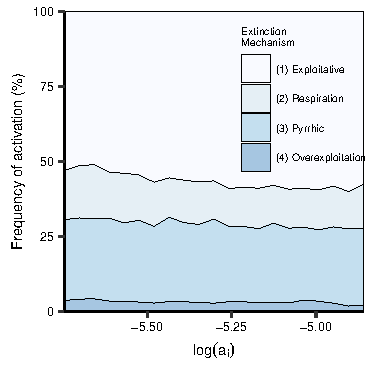
\includegraphics[scale=1.4]{../Images/activation_frequency.pdf}
  \caption{Activation frequencies of extinction mechanisms as functions of base attack rate
for respiration, over-exploitation, exploitative competition and
specialist competition. The frequency of activation is calculated for attack rates that fall between the 2.5$\%$ and 97.5$\%$ percentiles of the distribution of attack rates in the steady state of the model. This is achieved by sorting $a_i$ in to pre-defined bins of $\log_{10}(a_i)$ whose sizes are 5$\%$ of the total range recorded over the simulation. To calculate the frequency of activation of each respective extinction mechanism I divide (a) the probability of activation per bin (sum of the total number of extinctions divided by the sum of all lifetimes) by (b) the total probability of extinction per bin (sum of the respective probabilities of all mechanisms). \label{fig:frequency}
}
\end{center}
\end{figure}

\paragraph{Exploitative competition} The negative feedback produced by serial extinction is the most crucial component for understanding why consumers with larger $a_i$ are weaker with regards to exploitative competition. I firstly separate the exploitative competition inequality into components as
\begin{equation}
A=(\sum_{k=1}H_{kj}-1);\,\,B=\sum_{k=1}H_{kj}^{2};\,\,C=(\sum_{k=1}^{S_{\mathrm{R}}}H_{ki}-1);\,\,D=\sum_{k=1}H_{ki}H_{kj}\label{eq:comps}
\end{equation}
such that the inequality can be expressed as
\begin{equation}
\log_{10}(B)-log_{10}(A)+\log_{10}(C)-\log_{10}(D) < 0 \label{eq:exploitative_comp2} 
\end{equation}

where A and C represent the rescaled growth of consumer species in isolation. B and D respectively represent the intra and inter specific competitive. To understand why species with larger $a_i$ are more likely go extinct I  show how the distribution of each component varies with $a_i$ in Fig.~\ref{fig:comp_decon}. I have excluded the distribution of the joint components $\log_{10}(\frac{A}{B})$ because it depends entirely on the competitor $j$ and is thus unaffected by $a_i$ (see Fig.~\ref{fig:variation} (a) and (b) for a visual confirmation of this independence). Fig.~\ref{fig:comp_decon} thus serves as a visual tool for understanding the distribution of each component in the food-web, by averaging over may consumers during the steady-state. Fig.~\ref{fig:comp_decon} (a) firstly shows us that a larger $a_i$ is more likely to trigger the inequality in Eq. \eqref{eq:exploitative_comp2} given that $\log_{10}(B)-\log_{10}(A)+\log_{10}(C)-\log_{10}(D)$ decreases with $a_i$ (the increase in $a_i$ is depicted by the chromatic transition from blue to red). Comparison of Fig.~\ref{fig:comp_decon} (b) and (c) then tells us that most of the variation of (a), and indeed the shift in distribution from left to right for ascending $a_i$, is caused by component D. This is  what causes consumer species with larger $a_i$ to be weaker competitors in the long-run. Fig.~\ref{fig:comp_decon} (b) tells us that component C slightly decreases with $a_i$, contrary to the naive expectation given that at the point of invasion this component should increase with $a_i$. However, as discussed earlier in Sec. \ref{sec:serial_ext}, this decrease can be explained by the negative feedback caused by the serial extinction process, which I have replotted in Fig.~\ref{fig:comp_decon} (d). \\

% Graph created in final_paper_graphs_2.R
\begin{figure}[H]
 

\centering{}
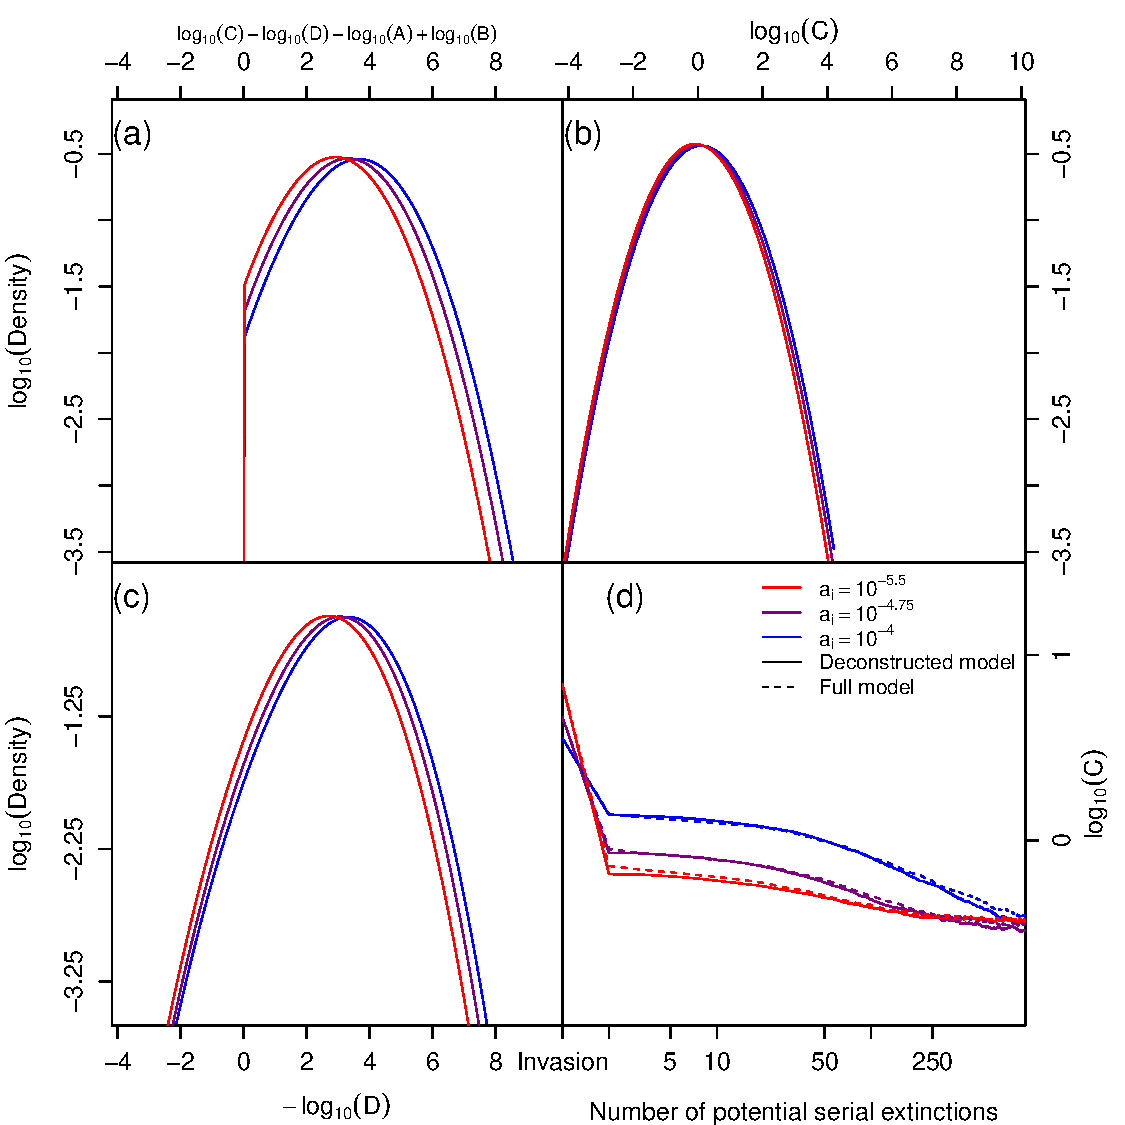
\includegraphics[scale=0.75]{../Images/components_with_without_serial_scaled_older.pdf}
\caption{Panels (a), (b) and (c) represent the distribution of the respective component of Eq. \eqref{eq:exploitative_comp2} obtained directly from the deconstructed assembly simulation (plotted using the density function in R with the bandwidth parameter set to 0.5). Panel (a) has been truncated past the threshold value of 0 because populations that reach values beyond this point go extinct. Figure (d) depicts the change in $\log_{10}(C)$ (y-axis) for fixed values of attack rate according to the cumulative number of resource additions (x-axis) averaged over 1000 replicate consumers obtained using the algorithm in Sec. \ref{sec:ser_ext}. The initial sampled set of resources to overcome respiration is denoted as “Invasion” on the x-axis, all other values reflect the change according to repeated serial extinction events driven by the addition of new resources. The full model values (dashed lines) correspond to the numerically integrated Lotka-Volterra equations (using ODE solver function “ode” in the “deSolve” package using the default solve method and tolerance setting, and 5000 maximal integration steps). The deconstructed model curves (solid lines) are calculated using the serial extinction algorithm in Eq. \eqref{eq:serial_extinction}. \label{fig:comp_decon}}.
\end{figure}

Fig.~\ref{fig:comp_decon} therefore explains why on average species with larger $a_i$ are more vulnerable to exploitative competition: For a fixed competitor $j$, such that $\log_{10}(B)-\log_{10}(A)$ is fixed, given that $\log_{10}(C)$ and $-\log_{10}(D)$ both decrease with $a_i$, the inequality in Eq. \eqref{eq:exploitative_comp2} is more likely to be activated. To get a more granular view of the dynamics that cause extinctions, I have plotted how the distribution of these components change with the number of resources added in Fig.~\ref{fig:variation}. I constructed this figure by randomly sampling a pseudo-competitor / invader during every resource addition in the serial extinction algorithm discussed in Sec. \ref{sec:serial_ext}. The resultant change in the components of the exploitative competition inequality, given the addition of a new resource and consumer, is depicted in Fig.~\ref{fig:variation} for two different $a_i$ values (left and right column respectively). I chose to show changes for each component in this way, because by fixing base attack rates and the number of resources for the component values calculated, I can provide a controlled comparison between $a_i$ values.

% Graph created in final_paper_graphs_2.R
\begin{figure}[H]
\centering{}
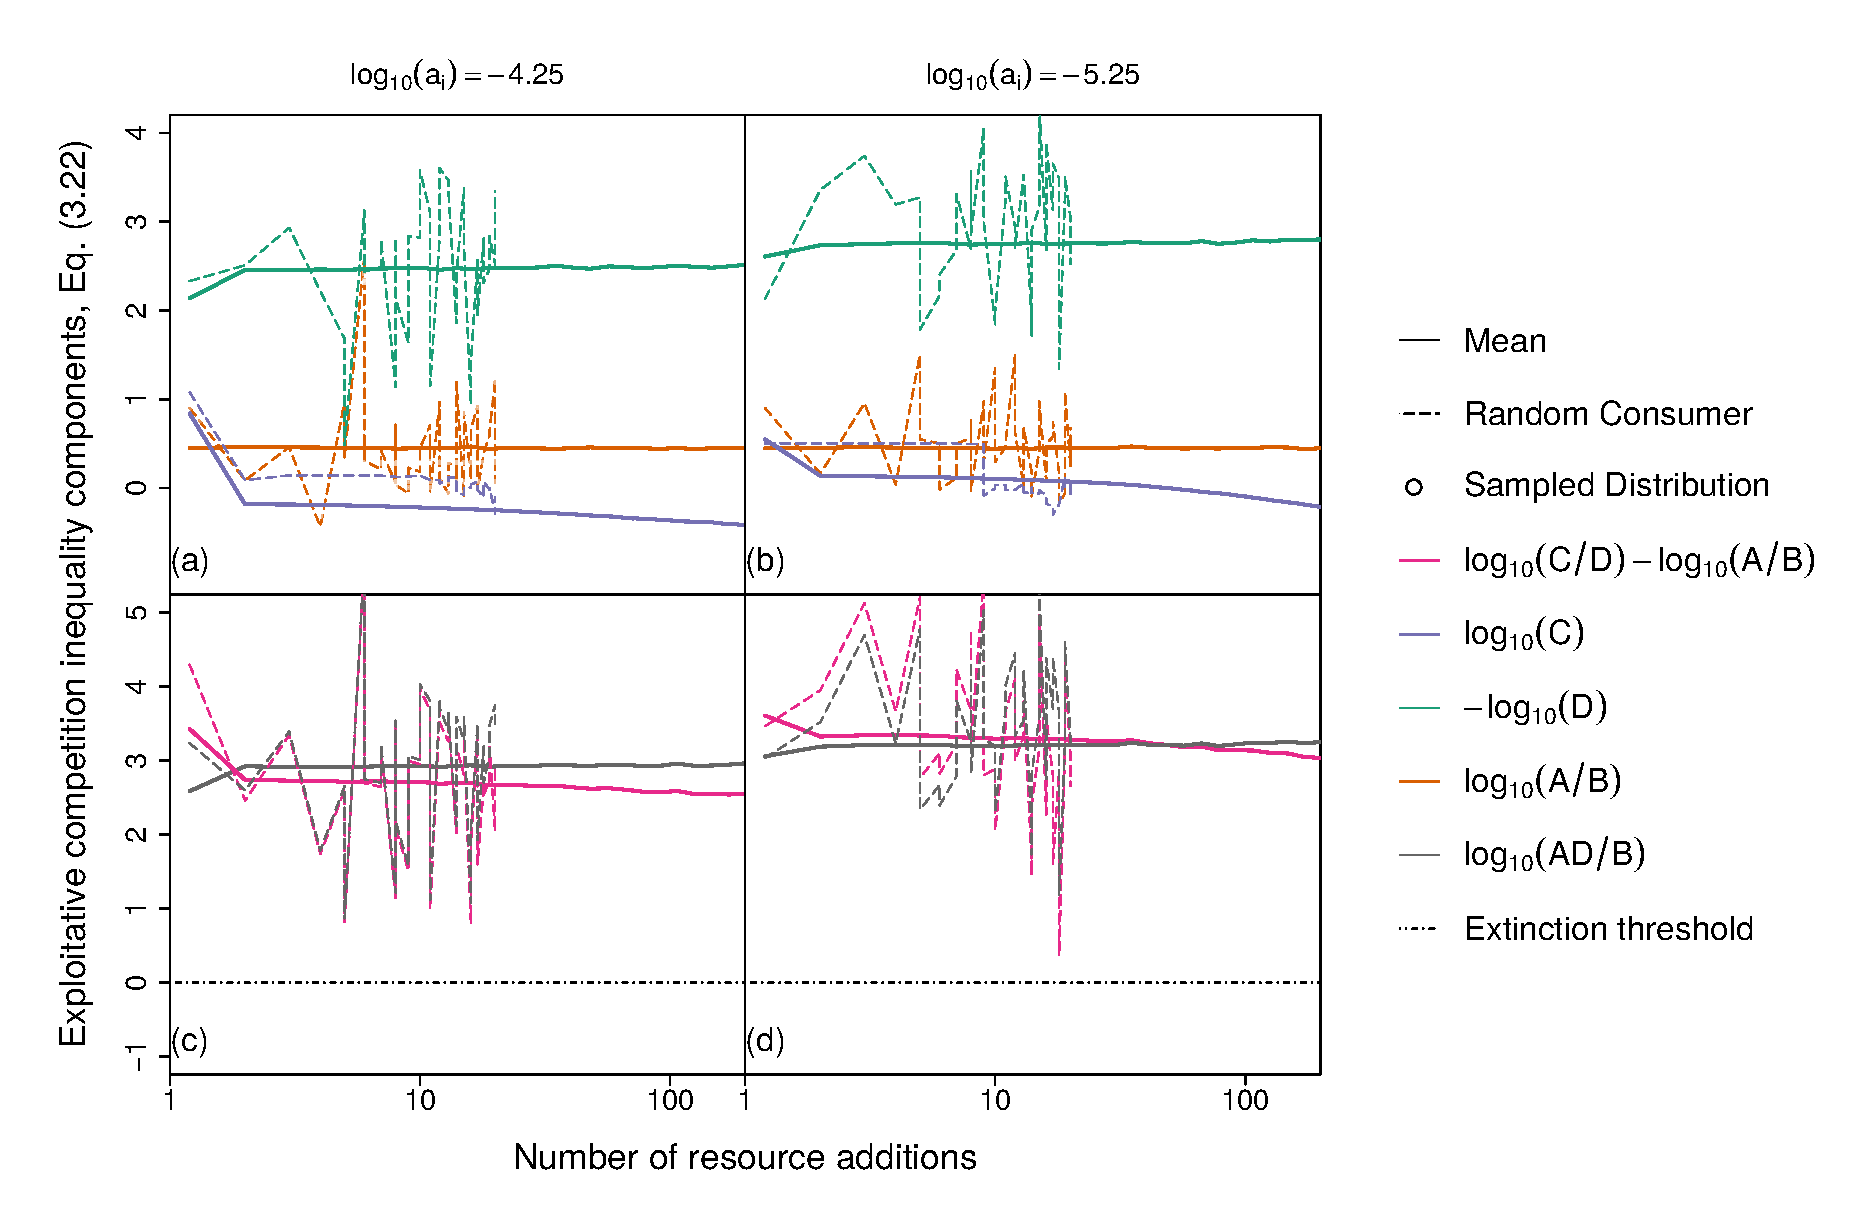
\includegraphics[scale=0.6]{../Images/variation.pdf}
\caption{I show how the respective components of exploitative inequality in Fig. \ref{fig:comp_decon} change through time due to the addition of resources (according to the serial extinction validation algorithm provided in Sec. \ref{sec:ser_ext}), and therefore, possible iterative activations of serial extinction. I plot these graphs for two fixed values of $a_i$ (left and right columns respectively) to show how these changes are dependent on the base attack rate of the species. The x-axis shows the number of resource addition events and thus represents the number of attempted serial extinction activations induced by adding resources. The solid lines are calculated using the same simplified serial extinction algorithm used to show the saturation of component C in Fig. \ref{fig:comp_decon} (and thus the corresponding number of replicates are identical). The dashed lines depicts the time-series of these components for a randomly sampled consumer used in the calculation of the mean, to give a sense of how each component may vary through time for an individual. I chose to limit the x-axis range of the dashed lines because when plotted on a logarithmic scale, including all time-series point after a threshold time-signature makes the resulting plot confusing to look at. I think plotting these lines before this threshold point is an acceptable solution given they are only mean to serve as a visual guide for the typical, individual specific, change in time for each component. Respective comparison of boxes (a) and (b) with (c) and (d) show how most of the variation in the exploitative competition inequality is accounted for by $\log_{10}(D)$. Furthermore, the mean is largely controlled by the mean of $\log_{10}(C)$. This is because as the resources are added, the mean of $\log_{10}(C)$ changes faster than that of $\log_{10}(D)$ and thus controls the change in mean of $\log_{10}(C/D)-\log_{10}(A/B)$, bringing it closer to the extinction threshold. By comparing left and right columns we see that the approach to extinction threshold occurs faster for larger $a_i$. The proximate cause of consumer extinctions is therefore $-\log_{10}(AD/B)$. The ultimate cause, which qualitatively explains the lifetime distribution of $a_i$, is due to the fast / slow decrease of $\log_{10}(C)$ over time with $a_i$ during / after establishment.
\label{fig:variation}}
\end{figure}


  In Fig. \ref{fig:variation}, panels (a) and (b) firstly show us that $\log_{10}(\frac{A}{B})$ is independent of competitor $i$, this is because this value depends entirely on the competitor $j's$ base attack rate, $a_j$. Second it is important to emphasise the following: If we sample through consumers $i$, but fix their competitor $j$, such that $a_j$ and $\log_{10}(\frac{A}{B})$ are fixed, Eq. \eqref{eq:exploitative_comp2} tells us that if C decreases and / or D increases (as we sample consumer's $i$), the chances of extinction of the competitor species $i$ increases. Now if we fix $a_i$ instead of $a_j$, and sample the competitors $j$, such that $C$ is fixed, although C and D are positively correlated (given they are both increasing functions of the set of trophic links of $i$), D can be considered as a random variable as we sample different competitors $j$ (because it is significantly affected by the amount of overlap between $i$ and $j$). Indeed this is why the variance of $D$ is much larger than that of $C$ with every resource and consumer addition. To see this compare the green dotted line (the time-series of a randomly sample consumer) to the solid line (the mean over all consumers) in Fig.~\ref{fig:comp_decon} (a) and (b)). Therefore although the means of C and D are positively correlated, the variation surrounding D makes their pair-wise correlation (i.e every $i$ $j$ competition paring) negligible. \\

Now consider the difference in means of $\log_{10}(D)$ with respect to the different base attack rates as negligible compared to their surrounding variance. Then, after the first serial extinction event, the combination of $-\log_{10}(D)$ and $\log_{10}(\frac{A}{B})$ (i.e $-\log_{10}(\frac{AD}{B})$) can be imagined as a random variable whose mean is largely invariant over time (measured as the number of resources is added). Thus, extinction occurs when $-\log_{10}(\frac{AD}{B})$ is small enough relative to $\log_{10}(C)$, which slowly decreases over time, and crucially does so faster as $a_i$ increases. The proximate cause for extinction are therefore the "jumps" in $-\log_{10}(\frac{AD}{B})$, that occur due to species turnover. Ecologically these "jumps" occur via consumer and resource turnover. The ultimate cause for increased vulnerability to extinction with increasing $a_i$ is the serial extinction process. Firstly because with increasing $a_i$, the subsequent decrease in $\log_{10}(C)$ makes the exploitative competition inequality defined in \eqref{eq:exploitative_comp2} likely to be crossed. Secondly, because the serial extinction component is the mechanism that accelerates the decrease of component $\log_{10}(C)$ over time as $a_i$ increases.


\section{Conclusion}

My objective for this chapter consisted in identifying how the evolution of trophic interaction strengths is constrained in a consumer-resource bi-partite food-web assembly. I firstly highlighted that species with intermediate trophic link strengths are fittest. I achieved this by defining the fitness of types as a function of mutant birth rate $b(a)$  and lifetime $L(a)$, and validated this in accordance with the Price equation. I was then able to explain the existence of a evolutionary steady-state via the interaction of the mutation bias and the emergence of the live-fast die-young trade-off. This trade-off penalises the initial advantage of increasing $b(a_i)$ by decreasing $L(a_i)$, such that on average $a_i$ reaches quasi-equilibrium when these terms (along with the mutation bias and standing variance) cancel each other out. \\

A mechanistic derivation of $b(a_i)$, i.e. Eq. \eqref{eq:birth_rate_final}, was achieved in Sec. \ref{sec:mech_det} via a convolution of the invasion probability of mutant species (which is based on the invasability criterion as shown in Sec. \ref{sec:inv}) and the probability of generating mutant species of type $a_m$. This completed the mechanistic derivation of the first part of the trade-off responsible for mitigating overexploitation. This first part describes how species with larger attack rates are initially favoured at the point of invasion and thus for dispersing in a metacommunity. A complete mechanistic quantitative derivation of $L(a_i)$ was not possible to achieve. Instead I set out to explain the qualitative decrease of lifetimes with $a_i$. I focused on the exploitative competition module given that this was the most frequently activated extinction mechanisms.\\

I discovered that the serial extinction process is responsible for penalising consumers with higher $a_i$ relative to this extinction mechanism. I achieved this by showing how component $C$ of the exploitative extinction threshold in Eq. \eqref{eq:exploitative_comp2} can be viewed as a threshold value that decreases with $a_i$, and further decreases as more resources are added. At a fixed point in time and for a fixed consumer $i$, such that component $C$ is fixed, the combination of all other components therefore acts as a random variable (if we consider each possible competitor as a random sampling event). The combined value of this random variable causes the extinction of $i$ if it is small enough relative to $C$. Given $C$ decreases with $a_i$ immediately after the invasion due to the serial extinction process, species with larger $a_i$ are more likely to go extinct due to Exploitative competition. This is not hindered by the eventual saturation of component $C$ because it makes many resource additions for this to occur. In fact, Fig. \ref{fig:comp_decon} shows us that it takes roughly 500 resource additions (equivalent to 500 time-steps) which is 5 times more than the average lifetime of consumers (roughly 100-150 time-steps). Even at the point of saturation of $C$, higher $a_i$ would still imply a higher chance of extinction because component $D$ (which increases the chances of activating extinctions) increases with $a_i$. \\
 
I argue that serial extinction is the ultimate reason for why species with higher base attack rate have a shorter lifetime within the food-web studied in this chapter. This is because the serial extinction process weakens species types with higher base attack rate, such that they are more likely to be outcompeted according to the Exploitative competition module. This is a more nuanced explanation than the naive expectation I had when I began investigating the central question of this thesis. I initially though that the decrease of $L(a)$ with $a$ would be due to the latter increasing the chances of activating and the overexploitation module defined in Sec. \ref{sec:res_over}. This is equivalent to the typically attributed evolutionary suicide induced by resource overexploitation. However Fig. \ref{fig:variation} tells us that this module is rarely activated.\\

The interplay of birth rate, lifetime and mutation bias is therefore essential to curb the evolutionary trajectory of base attack rates. The mutation bias is independent of the birth rate and lifetime, where the latter are intrinsically linked via a negative correlation. I call this effect the  live-fast die-young trade-off. I state that the interaction of the live-fast die-young trade-off with the mutation bias mitigates evolutionary suicide induced by overexploitation, in complex consumer-resource assembly models. It is important to highlight that the mutation bias is not an explicit constraint. This is because it does not directly modify the invasion fitness of species (i.e. the sign and magnitude of Eq. \eqref{eq:LV_consumer1} at the point of invasion). Instead it simply shifts the mean over which base attack rates are sampled and thus allows base attack rates to evolve to systematically increase if they are fitter. This is the cases where initial base attack rates are lower than the value at the steady-state. Indeed the strength of the mutation bias is moderated by the selection pressure at the point of invasion, i.e. the slope of the invasion probability function. Thus, the effects of the mutation bias are only significantly felt once the invasion probability is near saturation, which indicates a low selection pressure. This is the point in which we would expect the mutation bias to play a significant role in changing the frequencies of alleles, genotypes and resultant phenotypes not under selection.\\

 It is important to note that the mutation bias does not set the scale of base attack rates, this is instead set by the following  processes: Firstly, serial extinction limits the advantages of being larger $a_i$ for residents, such that beyond a certain value, larger values do not help much with increasing $b(a)$. One could therefore expect that for large $a$ the $b(a)$ curve in Fig. \ref{fig:fitness-decomposition} to become flat. Secondly, larger $a_i$ is detrimental to $L(a)$ lifetime once a species has invaded. We see how the $L(a)$ curve in Fig. \ref{fig:fitness-decomposition} bends downward. Therefore even without the mutation bias, the saturation of $b(a)$ and downward slope of $L(a)$ imply there is a real maximum of $R(a)$ at a somewhat larger $a$ currently reported. For both effects, the flattening of $b(a)$ and the downward bending of $L(a)$, the order of magnitude of the $a$ where this happens is given by the the values of $a$ where serial extinction becomes a common phenomenon. In this sense, serial extinction explains the limit to the increase of $a$. The mutation bias is necessary to increase the distance between the fitness maximum for $a$, and the value where all resource are eventually extinguished by invaders. These need to be separated on the $\log_{10}(a)$ axis (via the mutation bias) such that the consumers at equilibrium do not overexploit their resources. Note therefore that all three factors must be realised to achieve equilibrium, i.e. the mutation bias, the saturation of $b(a)$ and decrease of $L(a)$ with $a$.\\

In the next chapter I will test whether the live-fast die young trade-off in Eq. \eqref{eq:R-factorise} is robust to the advent of conspecific patch invasion. In this setting, populations of the same species may invade to outcompete one another, which may therefore enhance the fitness of types with larger base attack rates and possible destabilise the equilibrium achieved by the live-fast die-young trade-off.

\chapter{Robustness of the "live-fast die-young" trade-off in a metapopulation model. \label{ch:chapter_4}}

\maketitle

In the previous chapter I discussed how attack rates are constrained via an emergent trade-off between persistence and invasive fitness in a consumer-resource community assembly model (henceforth referred to as the 'local' model). Up until now I have disregarded the possibility of cheaters however, i.e. invading population that are identical to resident consumers, except that they have higher base attack rates. In this chapter I will address these shortcomings by including cheaters in a simplified metapopulation model which will be informed by the local model studied so far. The simplified metapopulation model therefore represents a patch network of connected local models. In this way I confront the mechanisms proposed to constrain attack rates studied in chapters 2 and 3, with intra-specific evolutionary forces that occur as a result of selection between populations of the same species as they disperse between local models. \\

\section{Introduction}
\label{sec:evol-metap-model}

%See also \url{https://scholar.google.co.uk/scholar?hl=en&as_sdt=0%2C5&q=evolutionary+%22metapopulation%22+model+suicide&btnG=}.

 The local model studied in the previous chapter - which is itself also a simplification of a metacommunity - ignores two crucial components that when combined could potentially affect the fitness of types, and therefore the ability of the identified mechanisms to mitigate overexploitation. The first is the approximation of the metacommunity as a single community. The simplification is implied via the algorithm for sampling trophic links, such that the base attack rates of invaders are sampled from within the food-web but are imagined to be sampled from surrounding imaginary patches. The second is the use of randomly sampled terms $\xi_{ij}$ to simplify the determination of attack rates by the vulnerability / foraging traits of the resources / consumers. In the local model, all trophic niche information would seem to be lost  when an invader is sampled from an imaginary nearby patch. However, the justification is that the invading species is not a descendant, but rather a close relative of a resident species. The information therefore is not actually lost during the invasion from the neighbouring patch, but during the entire evolutionary time separating the resident and related invading species. Now, imagine if we explicitly simulate many interconnected local model assembly simulations, and allow species invasions between these. In this setting the invasion fitness of relatively larger base attack rates should be enhanced if trophic information is now retained between invasions, i.e. if populations that share a similar niche may outcompete one another. Consider a mutant strain $j$ that attempts to invade a patch $p$ for example. If within patch $p$ there is a population $i$ of the same species (i.e. if $e_{ki}=e_{kj}$ $\forall k$) the exploitative competition inequality in Eq. \eqref{eq:exploitative_comp2} simplifies to
\begin{equation}
\alpha_i<\alpha_j \label{eq:exploi_2}
\end{equation}

 which will always be satisfied if $a_i<a_j$. I refer to this scenario as intra-specific exploitative competition. The population that outcompetes the other conspecific rival according to Eq. \eqref{eq:exploi_2} is the "cheater" in this scenario. Including these dynamics will ensure that we understand the robustness of the hypothesis presented this thesis. Explicitly using the local model to approximate intra-specific exploitative competition is not straightforward however. One could model the evolution of residents $a$ driven by intraspecific exploitative competition by adding mutants of the residents with the same set of trophic interactions (i.e. no re-sampling of trophic interactions upon invasion). However, to approximate the rate of invasion of populations of the same species into the food-web, we must make assumptions with regards to how each species is distributed in the imaginary metapopulation (in which the focal patch being simulated resides in). Three factors would need to be taken into account in such a model: (1) The relative magnitude of the typical duration $L$ of residency in a community, (2) the typical time between invasions of closely related species, both of which may depend on $a$, and (3) the effective distribution of the attack rates of "mutants" that results from metapopulation level selective processes. It is not clear how to derive these three factors without having to explicitly simulate the metacommunity itself. In this chapter I argue that one can circumvent having to explicitly simulate a metacommunity by inferring rates of invasion and extinction from the local model into a simplified metapopulation model, referred to as the "metapopulation" model henceforth.
 
 \section{General algorithm for the metapopulation model}
 
 The metapopulation model is created by combining the $N \times N $ patch set up of square lattice parasite-host metacommunity of \citep{Goodnight2008} with the dynamics of the classic stochastic patch occupancy model of \citep{Levins69:_DemographicGenetic}. Instead of each patch representing a host as in \citep{Goodnight2008} (which is either susceptible, infected by a population of the parasite species or deceased from an infection), each patch, characterised by Cartesian coordinates ($i,j$), will instead represent a local assembly model studied in chapter 2 and chapter 3. Each patch is then either occupied or not by the population of a consumer species dispersing in the simplified metacommunity. Rates of local extirpations and dispersal of populations in the metacommunity are modelled as a Markov processes depending only on patch occupancy, dispersal $D$, and patch specific base attack rate values $a_{ij}$. Because each patch is assumed to represent a local assembly model during its steady states, the rates of successful invasions and local extinction are rendered according to functions of base attack rates that reflect those observed in Fig. \ref{fig:fitness-decomposition} and studied in chapter 2 and chapter 3. If a patch was previously occupied, but the population has gone extinct for reasons other than intraspecific exploitative competition, new invasions will are achieved assuming the local communities of resources and competing consumers have substantially changed. Subsequent new invasions will occur according to the invasion probability interpolated from the community assembly model. The dynamics unfold according to the following algorithm:

\begin{enumerate}

\item Create a $N\times N$ Cartesian grid in which each site $i,j$ can be occupied (or not) by a population of the focal species identified by base attack rate $a_{ij}$ (I choose the initial values to be $10^{-5}$).

\item Set an initial number of populations (and corresponding initial $a_{ij}$ values) as a percentage $p_0$ of the total number of patches in the grid. 

\item Choose a population of residents in each patch to disperse according to a probability $D$ that is independent of base attack rates $\log_{10}(a_{ij})$. 

\item For each mutant chosen to disperse, attempt an invasion in an adjacent patch (chosen at random) by sampling the new base attack rate of the mutant according to Eq. \eqref{eq:attack_dist}. Then proceed according to whether:

\begin{enumerate} 

\item The attempted site for invasion already is occupied by a different population of the focal species with a larger base attack rate, if so the invasion attempt is considered to have failed.

\item The attempted site for invasion already is occupied by a different population of the focal species with a smaller base attack rate, if so the base attack rate of that site is then replaced by the mutant's larger base attack rate. 

\item The attempted site for invasion already is not occupied. In which case the new mutant will successfully invade according to Eq. \eqref{eq:prob_invasion}. For each invasion attempt sample a value of $S_R$ that is representative of the range found at equilibrium in the deconstructed assembly model and calculate $y_E$ and $\sigma_E$, the respective numeric estimated mean and standard deviation of the invasion probability Eq. \eqref{eq:birth3}. (Note: If a site was previously occupied but the resident has since gone extinct without being replaced, we assume that when a new mutant attempts to invade it, consumer and resource turnover have occurred in such a way that the invasion probability independent of previous occupancy).
\end{enumerate}
\item Sample which residents will go extinct according to the hazard defined defined by Eq. \eqref{eq:death_rate}, by sampling $u_{ij}$ from a uniform distribution that ranges from 0 to 1 for each resident. If $u_{ij}$ is smaller than the value of Eq. \eqref{eq:death_rate} given for that each respective base attack rate $a_{ij}$, the respective resident is removed such that the patch it occupied is free to be occupied according to 4. (b).
\item Repeat 3 - 5 for the desired simulation time.
\end{enumerate}

  Mutants may only disperse to patches that are directly connected to the patch $i,j$ they are dispersing from i.e. either $(i-1,j)$, $(i+1,j)$, $(i,j+1)$ or $(i,j-1)$. Mutants cannot invade beyond the boundary, instead their dispersal is restricted to any other available patches that are directly connect to it. 
  
\subsection{Assumptions regarding the simplified metapopulation model}
 
  To continue I will establish important assumptions and thoroughly explain the thought experiment around which the metapopulation model is based. This is crucial both to avoid potential biases when constructing and parametrising the model and to minimise confusion. Firstly, imagine the local model studied in the previous chapters as its metacommunity equivalent, i.e. composed of many connected patches with one of these representing
the focal food-web assembly model studied in chapters \ref{ch:chapter_2} and \ref{ch:chapter_3}. At each time-step the patches allow the invasion into one another of either a consumer or a resource as depicted by Fig. \ref{fig:topology_2}:

\begin{figure}[H]
\centering{}
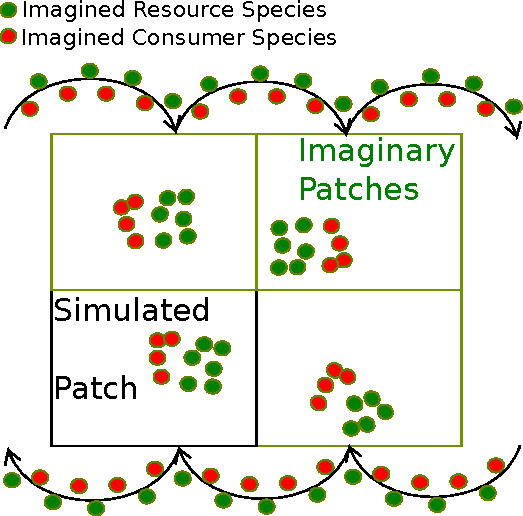
\includegraphics[scale=1]{../Images/topology_2.pdf}
\caption{Graphical representation of the community assembly model that simplifies the migration between a meta-community composed of $N \times N$ patches. The arrows symbolise migrations between patches of consumers (red dots) and resources (green dots). \label{fig:topology_2}}
\end{figure}

I now distinguishing two important conceptual developments that define the simplified representation of the metacommunity simulation. The first depicts the simplified metacommunity assembly before the introduction of intraspecific exploitative competition. I can safely assume that each initiated patch within the metacommunity with the initial conditions and parameters used in chapter \ref{ch:chapter_2} and chapter \ref{ch:chapter_3} assembles to reach similar steady-states in terms of the distribution of attack rates and the number of consumers and resources. This implies that the metacommunity retains no trophic niche information as in the local assembly model. Specifically, for each consumer and resource invasion, all trophic links are still sampled randomly, such that resource communities are assumed to be different in each patch. The only memory of the system is that of the base attack rates that are transferred between patches and subject to mutation as in the community assembly model. When all patches have assembled, such that they are at the steady-state described in the previous chapter, this will represent the initial state of the simplified metacommunity I study in this chapter. \\

The previous assumptions form the basis of the second important development of the simplified metacommunity model, that of cheaters being allowed to disperse in the simplified metacommunity model depicted in Fig.~\ref{fig:topology_3}. They describe the environment just before cheaters are suddenly allowed to disperse between patches. I therefore assume that the same rates of invasion and extinction can be applied to the simplified metacommunity, as long as I explicitly model extinction driven by cheaters. This is achieved via  intra-specific exploitative competition explained in Eq. \eqref{eq:exploi_2}, an in step 4 (b) of the metapopulation algorithm. I assume that the turnover caused by this novel type of competition does not disrupt rates of invasion and extinction derived from chapter 2 and chapter 3.

\begin{figure}[H]
\centering{}
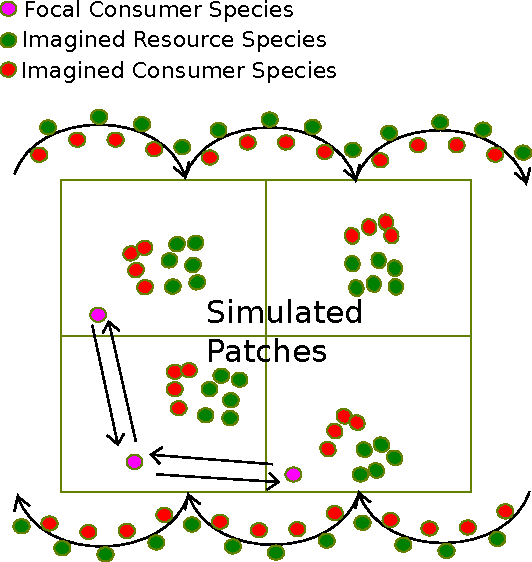
\includegraphics[scale=1]{../Images/topology_3.pdf}
\caption{Graphical representation of the approximated metacommunity community assembly in a $N \times N$ patch simulation. The arrows symbolise migrations between patches of imaginary consumers (red dots) and resources (green dots), and that of a focal consumer species (purple dot) whose populations disperse throughout the landscape. Each patch represents a food-web similar to that explicitly studied in chapter 2 and chapter 3 \label{fig:topology_3}}
\end{figure}

In the metapopulation models studied by \citep{Goodnight2008}, which forms the topological and ecological basis for the simplified metapopulation model, the parasite's ability to spread depends on their virulence and the availability of susceptible hosts in each patch (which form a $N \times N$ grid). The rate at which hosts die increases with virulence, leading to a trade-off between infection rate and persistence, that lets types of intermediate virulence be fittest in the long run. The authors go on to argue that by replacing parasites by consumers and hosts by resources, one might expect a similar negative feedback, such that consumers of intermediate foraging strength (so called "prudent predators") are fittest. The model presented in this chapter is slightly different to the analogy of \citep{Goodnight2008}, instead of replacing hosts by a specific resource, each patch instead represents a food-web community assembly model studied in the last two chapters, such that each patch experiences turnover via the invasion of resources and consumers. If persistence of the focal species is achieved in this simplified model, and if average base attack rates reach a steady-state (that is within a reasonable range studied in the original the community assembly model), this will be representative of the average dynamics of the entire meta-community. In which case I conclude that the  mechanisms studied in chapter \ref{ch:chapter_3} that mitigate overexploitation, are robust to dispersal and intraspecific exploitative competition, i.e. cheaters. In comparison, the modelling framework of \citep{Goodnight2008} is more abstract given it cannot immediately be linked to a local population dynamical model to that described in this thesis. The metapopluation model studied here is more specific given it is driven by the dynamics of the assembly model studied so far, i.e. the local model. This allows me to circumvent the need to use the simplifying assumption that there are only two interacting species. That said, the results in this chapter suggest that the mechanism at work in the two models are similar. I use the specific parametrisation of invasion probability $I(a)$ and lifetimes $L(a)$ derived form the local assembly model. I then show how the mechanisms originally alluded too by \citep{Goodnight2008} constrains the evolution of base attack rates (and therefore total trophic link strengths) and mitigates overexploitative behaviour. In this way, so called prudent predators (as coined by \citep{Slobodkin1968}) are fittest, via the emergent evolutionary  live-fast die-young trade-off. Before I explain these results I will explain how I infer the invasion probability and extinction rate of patches. 
 
\section{Definition of the invasion probability, hazard rate and dispersal rate}

Instead of inferring birth rates from the local model, I separate these into a dispersal rate $D$ (which is fixed throughout each simulation and which simulates the sampling of species selected to invade) and an invasion probabilities, which quantifies the ability to invade once chosen to disperse. The invasion probability of a species of type $\log_{10}(a_{ij})$ is obtained by turning the invasibility criterion $\sum_{k=1}^{S_{P}}B^R_ke^{\sigma\xi_{km}}a_{m}\epsilon<\rho$ (which was provided and validated in Sec. \ref{sec:inv}) into a probability distribution
\begin{equation}
P\Bigg[\sum_{k=1}^{S_{P}}e^{\sigma\xi_{km}}<\alpha_m\Bigg]\approx\Phi\Big(\frac{\ln(\alpha_m)-y_{0}}{\sigma_{0}}\Big)},\label{eq:prob_invasion}
\end{equation}
where $\alpha_m=\frac{a_m\epsilon K \beta}{\rho}$, $m$ represents a mutant attempting to invade a food-web with resident resources $k$, $\beta$ is the correction factor applied to account for resident competition at the point of invasion, and $y_0$ and $\sigma_0$ are the respective numeric estimates of the mean and standard deviation of $\sum_{k=1}^{S_{P}}e^{\sigma\xi_{km}}$. 

\subsection{Sampling new mutant $a_{ij}$ values} If a mutant population generated from a population located at $i,j$ successfully invades a patch $l,m$, then $a_{lm}$ will be sampled according to Eq. \eqref{eq:mutation} as in the local food-web model via
\begin{equation}
\log_{10}(a_{lm}) = \log_{10}(\gamma_{0}\gamma_{1}^{\xi}a_{ij}), \label{eq:attack_dist}
\end{equation}
where $\xi$ is a random variable distributed as $\sim N(0,1)$ at $\log_{10}(a_{lm} \times \gamma_{0})$ with standard deviation $\log_{10}(\gamma_{1})$. The mutation bias, $\gamma_{0}$, is exactly like that discussed in chapter 2 such that I assume that if there is lack of selection, the accumulation of deleterious mutations in a population (i.e. the mutational load) will lower the fitness of the population. 

\subsection{Hazard} The rate at which residents go extinct from each patch is obtained by assuming that life expectancy in the deconstructed and full assembly model can be approximated by a (constant) hazard model, such that the likelihood of a species reaching a certain lifetime, $L$, given a trait $a$, is given as
\begin{equation}
\mathscr{L}(L=t|a) = \prod_{i=0}^t (1-h(a)_i) h(a)_t \label{eq:likelihood_life}
\end{equation}
where $h(a)_t$, the hazard function, expresses the probability of species with trait $a$ going extinct at time $t$. If we assume a constant hazard, such that $h(a)_t=h(a)$ $\forall t$ Eq. \eqref{eq:likelihood_life} can be expressed as
\begin{equation}
\mathscr{L}(L=t|a) = (1-h(a))^{t-1}h(a)_t \label{eq:likelihood_life2}
\end{equation}
such that the expected lifetime, $E[L(a)]$, of a species with trait $a$ becomes 
\begin{equation}
E[L(a)] = \sum_{i=0}^{\infty}i(1-h(a))^{i-1}h(a)=\frac{1}{h(a)}. \label{eq:expected_life}
\end{equation}
Thus the hazard rates can be realised as 
\begin{equation}
h(a) = \frac{1}{E[L(a)]} \label{eq:death_rate}
\end{equation}
which can be obtained directly from calculations of $E[L(a)]$ from previous chapters (used to construct the curves in Fig. \ref{fig:fitness-decomposition} for example) as
\begin{equation}
E[L(a)] = \beta_0  + \beta_1 \log_{10}(a) + \beta_2 \log_{10}(a)^2 \label{eq:life_life}
\end{equation}

To calculate Eq. \eqref{eq:life_life} I first used a smoothing kernel\footnote{The function "rollmean" in R package "zoo" with bin sizes equal to $10\%$ of the number of input data points} to numerically estimate $E[L(\log_{10}(a))]$ over a fixed range of base attack rate values $(\log_{10}(a_{\min}),\log_{10}(a_{\max}))$ (see Tab. \ref{tab:parameters_meta}). I then proceeded to estimate $(\beta_1,\beta_2,\beta_3)$ via maximum likelihood estimation over this range by minimising the squared difference $(E[L(\log_{10}(a))]-\frac{1}{h(\log_{10}(a))})^2$.\\

\begin{table}[H]
  \caption{Fixed model parameters}\label{tab:parameters_meta}
\begin{tabular}{lll}

Symbol     & Description                                                                                                                                                                                                                      & Value                         \\
\hline
$\beta_0$  & Intercept for the hazard function Eq. \eqref{eq:death_rate}.  & 0.217 \\
\hline
$\beta_1$     & Linear term for the hazard function Eq. \eqref{eq:death_rate} & 0.074                            \\
\hline
$\beta_2$     & Quadratic term for the hazard function Eq. \eqref{eq:death_rate}                                                                                                                                                      & 0.006                              \\
\hline
$y_0$          & Mean of $\sum_{k=1}^{S_R} e^{\sigma \xi_km}$ term in Eq. \eqref{eq:prob_invasion} & 12                              \\
\hline
$\sigma_0$ & Standard deviation of $\sum_{k=1}^{S_R} e^{\sigma \xi_km}$ term  in Eq. \eqref{eq:prob_invasion} & 1                            \\
\hline
$S_p$     & Number of resources at quasi-equilibrium assumed for every patch & 250 \\
\hline
$\sigma$ & Inverse niche width & 4 \\
\hline
$\gamma_0$ & Mutation bias of base attack rate                                                                                                                                                                                           & $0.8^{0.5}$                           \\
\hline
$\gamma_1$ & Standard deviation of base attack rates                                                                                                                                                                                           & $1.3^{0.5}$                           \\
\hline
$p_0$     & Initial percentage of occupied sites & 10 \\
$\log_{10}(a_{min})$     & Minimal value used for interpolating hazard rates & -5.9 \\
\hline
$\log_{10}(a_{max})$     & Maximum value used for interpolating hazard rates & -4.7 \\
\hline
\end{tabular}
\end{table}

\section{Results}

In this section I will discuss the results describing the evolution of base attack rates and the proportion of occupied patches for a range of values of dispersal rate $D$ (which are fixed for each simulation). When $D^*=\frac{1}{S^*_C}\approx 0.004$ this is roughly equivalent to the rate at which consumers will invade a nearby patch (assuming all invasion attempts are guaranteed) if one consumer is sampled randomly from all other $S^*_C$ consumers within each patch. In Fig. \ref{fig:Meta_com_time_series_no_intra} I firstly show graphs depicting the simplified metacommunity simulation in which there can be no cheaters, such that if a patch is occupied, no other population may attempt to invade it even if it has larger base attack rates.

% Graph created in Orestes_metacommuntiy_grid.R
\begin{figure}[H]
\centering{}
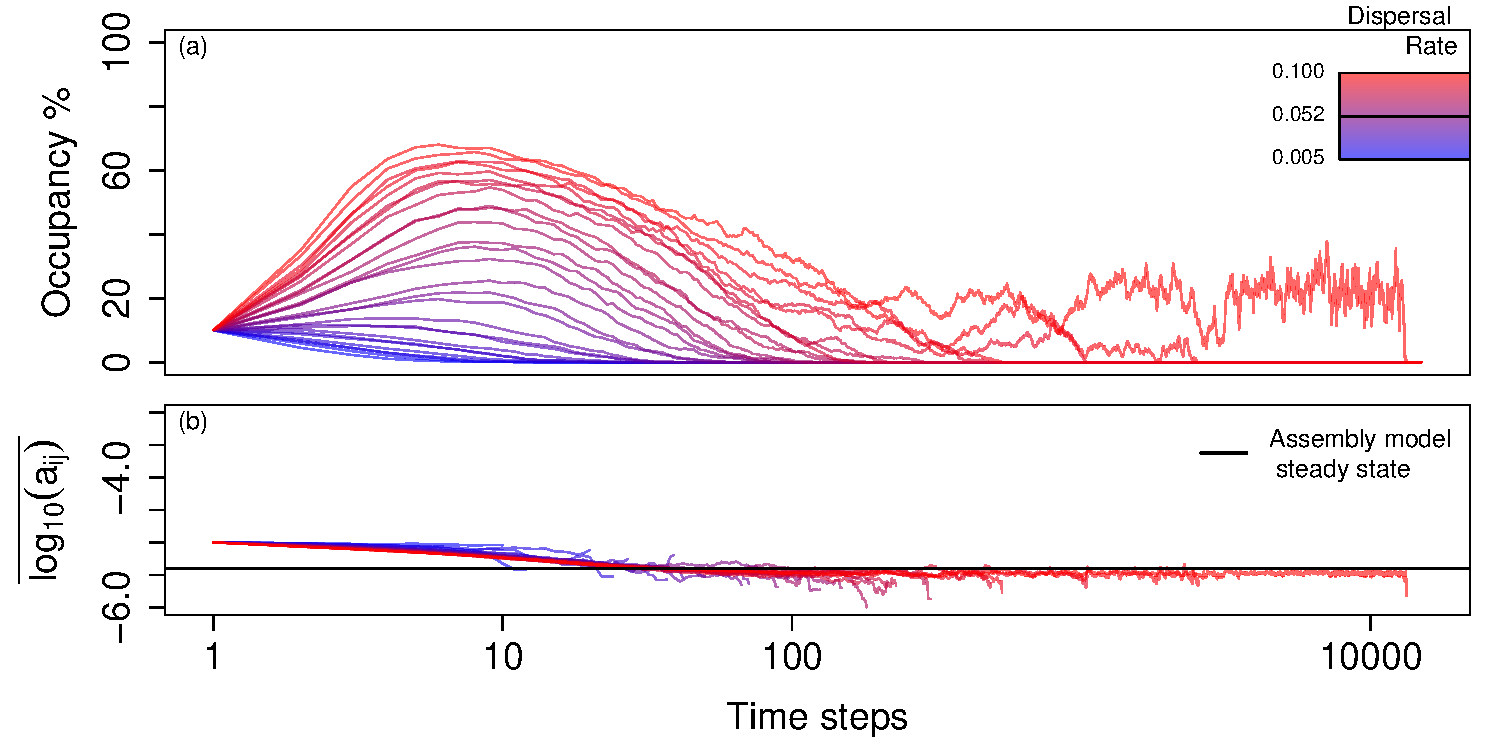
\includegraphics[scale=0.7]{../Images/Meta_com_time_series_no_intra.pdf}
\caption{Graphs for the time-series of the $\%$ of occupied patches (top) and $\overline{\log_{10}(a_{ij})}$ (bottom). \label{fig:Meta_com_time_series_no_intra}}
\end{figure}

 In panel (a) of Fig.~\ref{fig:Meta_com_time_series_no_intra} we firstly see that for all dispersal rates tested, patch occupancy will at some point equal 0$\%$. The average time it takes for this to happen is significantly delayed by the amount of dispersal $D$. From panel (b) we see that when cheaters are not present, average base attack rates recorded during the steady state saturate very near to the average value recorded during the steady state of the local assembly model studied in chapter 3\footnote{Although there is a slight difference this is attributable to measurement errors of the $\beta_0$, $\beta_1$ and $\beta_2$ parameters defining the death and birth rates used in the simplified metapopulation model}. This is what we would expected from the metacommunity model without cheaters. Fig.~\ref{fig:Meta_com_time_series_no_intra} therefore serves firstly as a validation tool to ensure the set up of the metapopulation model is correct. If it were not, there would be severe deviations between the saturation of base attack rates and the black line in Fig.~\ref{fig:Meta_com_time_series_no_intra} (b). It also serves as a benchmark tool to compare against the model variant with cheaters/intraspecific competition, which I present in Fig. \ref{fig:Meta_com_time_series_2}.
 
% Graph created in Orestes_metacommuntiy_grid.R
\begin{figure}[H]
\centering{}
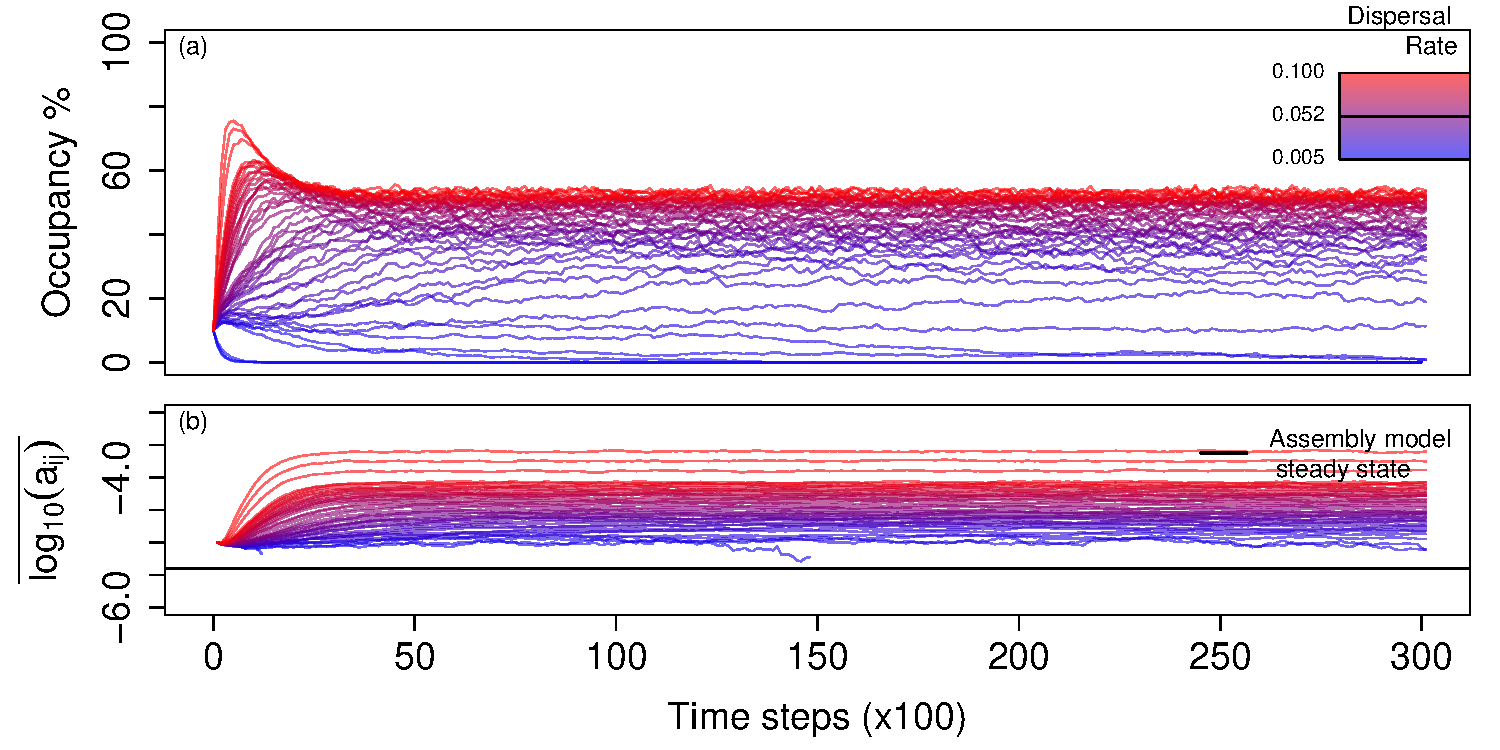
\includegraphics[scale=0.7]{../Images/Meta_com_time_series_2.pdf}
\caption{Time-series of the $\%$ of occupied patches (top) and $\overline{\log_{10}(a_{ij})}$. \label{fig:Meta_com_time_series_2}}
\end{figure}

Fig.~\ref{fig:Meta_com_time_series_2} (a) again informs us that if dispersal rates are not high enough, the focal species will soon go globally extinct and reach levels of patch occupancy equal to $0\%$. This global extinction occurs for values of $a$ above the mean studied in the local assembly model, but within the range in which it fluctuates during the steady state, and thus global extinction is not due to overexploitation of resources, but rather due to the typical dynamics driving consumers turnover (such as exploitative competition). As we increase $D$, such that populations do not go globally extinct, an upper limit seems to exist for patch occupancy.  Although the maximum level of patch occupancy also increases with $D$, the value during the steady state saturates at around $50\%$.\\

In Fig. \ref{fig:Meta_com_time_series_random} I show the equivalent version of Fig. \ref{fig:Meta_com_time_series_2}} for when patch connectance is completely random, such that for each dispersal attempt, populations are not limited to nearby patch and can attempt to invade any patch in the metacommunity. As we can see, the virtually random topology does not affect qualitative behaviour of the long term dynamics. Indeed, $\overline{log_{10}(a_{ij})}$ does not grow indefinitely for the range of fixed dispersal rates tested.\\ 

\begin{figure}[H]
\centering{}
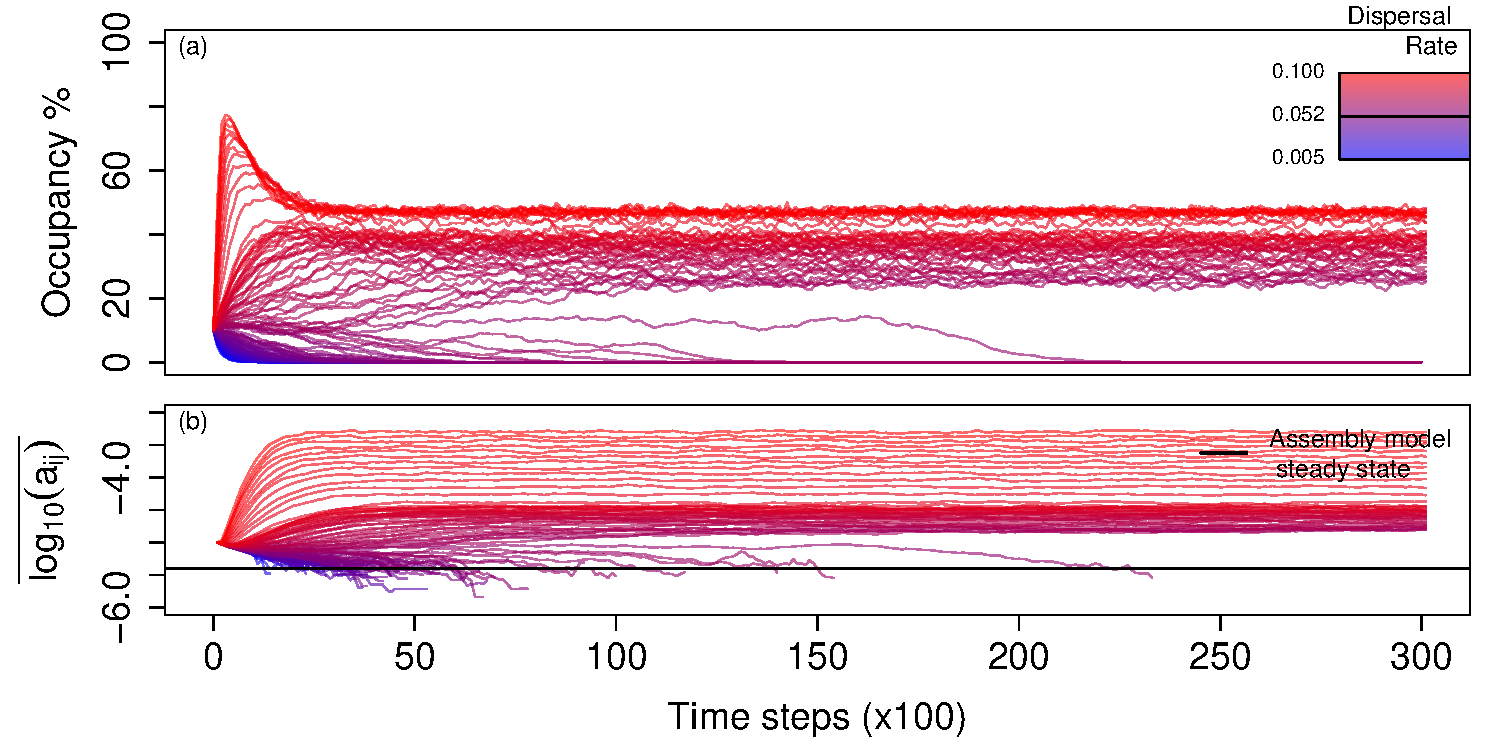
\includegraphics[scale=0.7]{../Images/Meta_com_time_series_random.pdf}
\caption{Time-series of the $\%$ of occupied patches (top) and $\overline{\log_{10}(a_{ij})}$ for a completely random patch connectance, such that populations can disperse to any patch in the $N \times N$ grid. \label{fig:Meta_com_time_series_random}}
\end{figure}

Comparison of Figs. \ref{fig:Meta_com_time_series_no_intra}  and \ref{fig:Meta_com_time_series_2} shows us firstly that patch migration clearly gives potential cheaters an evolutionary advantage, given that steady-state average base attack increases relative to the local assembly model. Secondly, during the steady-state, average base attack rates do not increase indefinitely as one might naively expected when incorporating cheaters. This implies that if we were to extend the current full and deconstructed assembly models to simulations of full metacommunities, the trade-off that we propose as constraining the evolution of base attack rates (and therefore overexploitation of resources) would not be mitigated by the advent of migration of intraspecific species populations. This indicates that patch migration of intraspecific populations does not override the evolutionary stabilising properties of the mechanism proposed in this thesis. Given the behaviour in Fig. \ref{fig:Meta_com_time_series_2} is reflective of what all other imaginary species are experiencing in the metapopulation, our model further predicts that on average all consumer species may still evolve in such a way that overexploitation is mitigated and trophic interactions constrained by the mechanisms discussed in this thesis. Thus whilst intraspecific competitive advantage associated with disperse may aid relatively larger base attack rates, this is not enough to usurp evolutionary forces that mitigate the evolutionary suicide induced by overexploitation. If this were the case, we would see a constant increase of $\overline{\log_{10}(a_{ij})}$ over time.\\

\section{Conclusion}

In this chapter I considered evolutionary forces - namely intraspecific exploitative competition - that occur from the selection between populations of the same species. These where not considered in the modelling framework in which the mechanisms constraining attack rates were originally studied. Instead of simulating the invasion of populations within assembly models studied so far (which simplify a metacommunity), I simulated a patch specific simplified metacommunity model that applies the extinction and dispersal rates studied in the last chapter. This allowed me to circumvent the need to assume the distributions of species types dispersing within a meta-community. This would require spatio-temporal averaging dynamics that depend on the short and long term fitness of types. This work was inspired by a parasite-host metacommunity simulation, modelled on a $N \times N$ patch system by \citep{Goodnight2008}. The authors discuses how an emergent trade-off that allows types of intermediate virulence to be fittest should not be spatially or temporally averaged and instead needs to be studied in an explicit spatio-temporal setting. Indeed \citep{Goodnight2008} suggest that the trade-off that is active in the parasite-host evolutionary history could be occurring analogously for predator-prey co-evolution, whilst their model is required to detect such a trade-off, in this chapter I used a similar model to test its robustness.\\

Instead of replacing hosts by a specific resource, as in \citep{Goodnight2008} analogy, I simulate a simplified metacommunity in which each patch represents a food-web community assembly model studied in the last two chapters. Under the assumption that each patch reaches the steady-state studied in previous chapters, I applied the invasion probabilities and extinction rates to simulate the dispersal of a species, composed of patch specific populations, within the meta-community. To achieve this I separated the sampling and invasion process of species into independent dispersal rates (independent of attack rates) and invasion probabilities (interpolated from the chapter \ref{ch:chapter_2} and chapter \ref{ch:chapter_3}). Finally, only the sub-population of a focal species of consumer (rather than many species) is simulated, under the assumption that it is representative of the average behaviour of all other imaginary consumers that are dispersing simultaneously in the meta-community.\\

The simplification  of a metacommunity, as detailed in this chapter, has two main advantages. Firstly, the division of consumer species into population means we do not have to to explicitly simulate foraging and vulnerability traits to capture the effects of intraspecific exploitative competition. Secondly, using the rate of extinction and invasion from the community assembly model avoids having to simulate species rich communities. Indeed without cheaters, Fig. \ref{fig:Meta_com_time_series_no_intra} depicts how the average base attack rates during the steady-state of the simplified metacommunity model are the same as in the one-patch model. \\

  I firstly concluded that patch migration allows cheaters to push average base attack rates above the steady state reported in chapter \ref{ch:chapter_3}, but that these still saturate around a constant average value during the steady state (see Fig.~\ref{fig:Meta_com_time_series_2}). Furthermore, although increased dispersal may increase the average value of base attack rates during the steady state, they do not increase indefinitely over time. This is what one might expect in a scenario in which many population compete over a set of limited resource, reminiscent of the tragedy of the commons first conceived by \citep{Hardin1968}. Thus the mechanism detailed in chapter \ref{ch:chapter_3} that renders a trade-off between invasive ability and persistence, which subsequently constrains consumer attack rates, is robust to the potential domination of cheaters. This is because the advantage of cheaters, relies on the percentage of occupied patches and the dispersal rates at their disposition. Higher values of $a_i$ may be selected as long as the sampled value is higher than that of an already occupied patch. Although the sampling of $a_i$ is subject to the mutation bias, this will only act to slow down the potentially unconstrained increases in $a_i$ associated with cheaters. However given that patches also go extinct more quickly as $a_i$ increases, it is also possible for a balance to occur such that levels of occupancy may be decreased to the point in which cheaters can no longer capitalise on patches with existing conspecific residents. This would seem to be the case according to Fig. \ref{fig:Meta_com_time_series_2} where indeed we see that as dispersal rates increase. This leads to a faster acceleration associated with increases in $a$, and also seemingly initially leads to higher levels of occupancy, after which occupancy declines as $a_i$ increases. The average value of $a_i$ does not show the same saturation with dispersal rates on the other hand, such that increasing dispersal rates will yield increases in the average value of $a_i$ during the steady state.  \\
  
  It would seem therefore that mitigation of overexploitation depends on dispersal rates, and that increasing these beyond a critical threshold would lead to values of $a$ that could cause a metapoulation wide collapse (i.e. for values of $a$ greater than the overexploitation threshold in Eq. \eqref{eq:over_exploitation}). However given that I have not explicitly modelled the local food-web dynamics occurring in this range of base attack rates I cannot interpret dynamics beyond certain values of $a$. It is even possible that some other hidden dynamic may saturate the increase of average attack rates measured during the steady-state. For example, the increase in death rates with $a$ may also accelerate with $a$, given that Fig. \ref{fig:fitness-decomposition} (d) and (h) experience an accelerated decrease with lifetimes as $log_{10}(a)$ increase. Furthermore, the current metapopulation simplification assumes that once a patch looses a population, the food-web within it is reset within that time-step, such that a new population attempting to invade is subject to the typical birth rate of a patch that has never been invaded by the species. Instead it would be more reasonable to expect these patches require a certain amount of species turnover to occur in order to recover from the niche deterioration caused by recently decease populations. In this way if not enough time has passed since a species was removed from a local patch, populations of the same species would find it difficult (or even impossible) to invade (especially for values of $a$ smaller than the previous resident, but also for larger values). This could be implemented in a simplified form by adding lag time in the form of an arbitrary number of time-steps before a patch becomes habitable again, or by amending  birth rates. However I decided not to include these potential biases. That the saturation of $a$ during the system steady state occurs, even when the niches of patches are completely reset after local extinction, is a clear enough indicator that the mechanism studied in this thesis is not overpowered by cheaters aided by migration between patches for the parameter regimes studied in chapter \ref{ch:chapter_2} and chapter \ref{ch:chapter_3}. \\
  
  Although I use a metacommunity to test the robustness of a trade-off for mitigating overexploitation, the model used to derive and study the trade-off is itself a simplification of a metacommunity. Therefore, the prediction of \citep{Goodnight2008}, that a spatio-temporal explicit treatment for studying evolutionary dynamics consumers and resources would reveal a fitness trade-off similar to that found in parasite-host communities seems to be correct. A negative feedback, caused by disrupting the very same resource pool that the consumers use to establish, forms trade-off between invasive ability and persistence. This live-fast die-young trade-off causes types of intermediate with attack rates to be fittest in the long-term. In the next chapter I will highlight the main ecological signatures expected to occur as a result of the live-fast die-young trade-off, and compare these expectation to field observations.
  
\chapter{Empirical signatures of the live-fast die-young trade-off\label{ch:chapter_5}}

\section{Introduction}

The mechanism identified in chapter \ref{ch:chapter_3} should be present and measurable in species competing over limited resources. It predicts that species evolve to live within limits imposed by their environments: the regenerative ability and diversity of niches. In particular I pose that this limit will be enforced by a negative feedback occurring at the population level, such that the long-term fitness of populations is defined by the live-fast die-young trade-off\footnote{Populations with stronger base attack rates are likelier to invade a community, however, they also erode their local niche the most and are therefore more likely to go extinct. The evolutionarily fittest populations in the long run are those that reach a balance between the ability to invade and persist}. It is therefore crucial to understand whether the expected live-fast die-young trade-off is indeed observable in natural food-webs. In the following chapter I will consider three different broad patterns in species traits and community structure predicted by the live-fast die-young trade-off. I will categorise these according to which stage they present themselves during the establishment of a population and compare them to existing ecological and evolutionary theory. The first category I discuss are for effects that occur “a posteriori”, i.e. after the invasion and establishment of species, and are thus the products of significant evolutionary changes that have been driven in a species. For this category I will limit myself to describing the expected patterns, given that clear empirical data or the adequate type was difficult to find. The second category corresponds to evidence for mechanisms arising during field observations. These will be organised into either three or four patterns, depending on whether the observations are for general ecological activity or if they are specific to the monitoring of species invasions (of which so called “boom-bust” invasions are of particular interest).

\section{“A posteriori” signatures: The saturation of $H_i$}

I begin by describing the indirect implication of the mechanism, which is directly related to the saturation of $H_i$ parameter in Sec. \ref{sec:model_definition}

\begin{equation}
H_i=\frac{\epsilon a_i \sum_{k=1}^{S_R}a_{ki}B^R_k}{\rho}
\end{equation}

I remind that $\rho$ is the combined rate of respiration and natural mortality. $\epsilon$ represents the conversion efficiency of assimilated resource biomass into biomass of the consumer. $a_i$ represents, for a consumer $i$, the base attack rate which is multiplied by $a_{ki}$, the trophic interaction with a resource species $k$. Fig. \ref{fig:serial_ext} in Sec. \ref{sec:serial_ext} implies that for those native species having undergone many serial extinction events, and which have subsequently settled and adapted to their environment, the value at which $H_i$ saturates is independent of $\alpha_0$. Given $\alpha_0$ is composed not only of base attack rates, but also respiration, $\epsilon $ and $K$ as well, this independence should exist for all the biotic parameters that compose $\alpha_0$. This implies that in the long-run $H_i$ saturates at a level that is independent of the biotic parameters that enter the serial extinction inequality, Eq. \eqref{eq:serial_extinction}. This implies that all species that have settled, are balanced with their environment, such that the value of $H_i$ becomes independent of species and their environment. This prediction can be tested quantitatively in two ways, the first is to replicate the serial extinction algorithm in Sec. \ref{sec:serial_ext} as an empirical experiment. This can be achieved by measuring the time-series of $H_i$ for a species entering a novel environment and subsequently verifying that $H_i$ indeed saturates after a variety of potential species that could be consumed by the focal consumer have invaded. This experiment would be analogous to the serial extinction algorithm detailed in Sec. \ref{sec:serial_ext} and would require a controlled experiment (the most feasible organism being at the scale of microorganisms) and a diversity of resources that could replicate the addition of resources in the assembly models. Another possibility is to confirm that native species in the same environment have similar values of $H_i$, or that younger arrivals tend to have larger values on average. Both these possibilities would be extremely complex to enact however. My prediction for saturation is based on the assumption that all resources species in the food-web have the same growth rate and carrying capacity and other simplifying model assumptions. A broader pattern that might be more easily observable concerns the fact that all these parameters should balance each other, such that in environments with relatively larger carrying capacity of resources, either attack rates will be lower or respiration higher (or a combination of these) than in environments with lower carrying capacity. 

\section{Signatures of the “live-fast die-young” trade-off \label{sec:signatures}}

The most important empirical observations are from studies that exhibit tell tale signs that indicate that the mechanisms underlying the live-fast die-young trade-off are active. Specifically, the expectation that “greedier” species (i.e. ones that are capable of relatively high predatory/foraging ability) are more likely to lose their most important resources. These consumers would subsequently be left to compete over resources they are not as well adapted to, and made locally extinct via exploitative competition. An ideal empirical study should exhibit the following signs:\\

%\renewcommand{\labelenumi}{\alph{enumi}}


\paragraph{(a)} That rate of growth of the population of a species within a community is negatively correlated with its ability to persist within it.\\

\paragraph{(b)} A negative feedback caused by serial extinctions: The ultimate cause of the negative correlation in (a) (and thus of local extinctions) is the overexploitation of the preferred self-limiting resource species of that focal consumer species, which is driven by serial extinctions. The subsequent reliance on other resources it is less well adapted to therefore weakens its ability to compete with other species.\\

\paragraph{(c)} The proximate cause of extinction should be exploitative competition of populations. This can be caused either by new invaders that can capitalise on the weakened previous invader that has deteriorated its niche, or by resident competitors that gained new resources through turnover of the resource community and so became more abundant.\\

The evidence and discussion of these phenomena can also be broadly organised according to the scale they might occur at:

\paragraph{I} In small homogeneous patches, once a species has entered one, the chances of dispersing between others patches are significantly smaller than between large heterogeneous patches (like woodland for example). Furthermore, when dispersing within it, a species will encounter the same environment. Examples of these patches, are ones in which species will spend their entire life-cycles occur in isolated patches (such as ponds), so that they cannot disperse from these. This would be the ideal example, because once the population has entered the patch, one can categorically identify whether its main resource has gone extinct, and if subsequently the focal population also went locally extinct. 

\paragraph{II}  In large heterogeneous patches, such as extensive terrestrial/aquatic environments (e.g. woodland, lakes, river systems), an invasive species can easily disperse between and within these and encounter a heterogeneous landscape. In these scenarios the trade-off becomes harder to identify simply because it is hard to show that the invasive species has eradicated its main resources. Given that it would take considerably more time than in the case of small homogeneous patches, it opens up the possibility of adaptation of both consumer and resource as well and of effects associated with species dispersal to confound the mechanism proposed in this thesis.\\

Most empirical studies tailor their measurements to suit specific ecological questions. The duration of observation and focus of biotic/abiotic characteristics is therefore specific to these questions. It is subsequently difficult to find evidence of signatures (a), (b), (c) in a single study. Next I will give an example of studies that qualitatively display some of the signatures, but that fails to explicitly display crucial aspects of it (and which therefore highlights the difficulty in finding good empirical examples). In the experiments by \citep{Johst2003}, the authors build on previous laboratory experimental studies for analysing the dependence of predator-prey persistence on patch connectedness, by analysing field observational experiment. Specifically, they discuss how the long-term persistence of the flightless weevil \textit{Hadramphus spinipennis} causes the frequent local extinction of its host plant \textit{Aciphylla dieffenbachii}. They highlight that the dependence on the ability of the consumer to disperse, occurs relative to the spatial and temporal scales of dispersal and patch use (e.g. regeneration, destruction). That the weevil manages to persist, despite its potential to overexploit its resources (that is modulated by patch connectance), indicates either an active feedback stops the occurrence of total prey exploitation, or that persistence occurs by chance (i.e. the parameters controlling the co-evolution of predator and prey are by chance fine tuned relative to extent of patch connectedness). The former assumption may be likelier, however it is not clear whether the types of weevil that cause local extinctions go extinct themselves (akin to the overexploitation mechanisms in Sec. \ref{sec:res_over}) or if they are indeed weakened by a reliance on secondary resources that make them more vulnerable to outcompetition and extinction. Thus it is not clear if this is a good example of signatures (a) through (c). However given measurements are from field observations, rather than a laboratory experiment, there are presumably other resources and indeed competitors of the weevil. \\

The best source of evidence, which I will focus on for the rest of this chapter, are studies on the impacts of invasive species on ecosystems. These are generally extensively documented qualitatively, such that a meta analysis by \citep{Sodhi2014} found that “out of 170 extinct species for which (extinction causes have been identified reliably), invasive species contributed directly to the demise of 91”. They note in particular that the threat of extinctions occurring on islands have been greatly increased due to non-native predators. They list several attributes that include the evolutionary advantage of predators relative to their preys traits (e.g. lack of flight in birds or lack of thorns in plants), and case scenarios such as the infamous introduction of the brown tree snake (\textit{Boiga irregularis}) that led to the extinction of many native species in Guam. This area of research therefore documents many cases of resource extinctions driven by predators and potentially contains investigations on the ability of these invasive species to persist after they have generated resource turnover. I will now elaborate on signatures (a) (b), and (c), such that they reflect the expected ecological impacts of species invasions and make them more comparable to these (mainly) qualitative, studies. Firstly, (a) should be qualitatively observable in an invasive species such that those with the most pest-like and destructive qualities, will be less successful at remaining established in non-native territory. They should exhibit “boom-bust” qualities, which is a term used to describe the mysterious disappearances (the “bust”) of invasive species that initially had experienced significant population growth (the “boom”). Furthermore, the population explosion of the invasive species may allow it to displace native species with similar (not necessarily identical) niches. Signature (b) should be observable via the exhaustion of its most important resources, such that it depends on resources that can no longer sustain the initial growth of the invader. This subsequently leads to the “bust”: the invasive species population reaches an equilibrium level significantly smaller than the peak it reached during its explosive growth. Signature (c) should be observable by the return of a previously displaced native competitor, whose most important resource was not exhausted by the invader, and can now capitalise on the significantly deflated population of the invader. This displacement may also be achieved by a new invader, that may not have been able to established during the arrival of the focal invader. This dissection of (a), (b) and (c) is summarised by the following steps therefore:

\begin{enumerate}

\item The “boom”: During invasion/establishment, consumer species can capitalise on available resources in such a way that their population explodes.

\item Other existing consumer species are outcompeted via the exploitative competition module detailed in Sec. \ref{sec:exp_comp}. This can occur even if their most important resource are different, however their niches must be similar enough such that the invasive species expels others sheer force of numbers.

\item In a relatively small time-frame (i.e. before any trait adaptation of either consumer or resources takes place), the population explosion causes severe degradation or extinction to the population of its most important resource (i.e. the “negative feedback” serial extinction process detailed in Sec. \ref{sec:serial_ext} ).

\item The “bust”: The population decline (or even extinction) of the preferred resource in 3 causes a subsequent decline of the invasive species population relative to its initial boom. The invasive species can now still survive but at a severely diminished level relative to its initial boom, given that it relies on secondary, less important resources that it is not as well adapted to.

\item The “final blow”: The reliance on secondary resources means that the focal consumer it is subsequently outcompeted (i.e. via exploitative competition detailed in Sec. \ref{sec:exp_comp}) from a patch, possibly by the same species it may have displaced during step 2.

\end{enumerate}

\section{Boom-bust species invasions}

To verify the mechanisms discussed in this thesis it is important to find research that chronologically displays steps 1 through 5. I will therefore discuss research relating to “boom-bust” invasion events (see \citep{Strayer2017} and \citep{Simberloff2004}, some of the examples of which I present below), whereby an invasive species initially grows very quickly in abundance and then decreases sharply in abundance, either going extinct or settling at much lower abundances. Boom-bust scenarios are consistent with signatures 1. and  4. However, whether these scenarios are consistent with signatures 2., 3. and 5. remains to be verified. \\

Not all studies of boom-bust dynamics in invasions are done with the same focus. Usually the original objective drives the authors to collect and analyse data in such way that direct comparison to these signatures is difficult. A good example of this problem is the study of invasive signal crayfish \textit{Pacifastacus leniusculus} that have spread in Swedish lakes since the 1960s. An analysis by \citep{Sandstro2014} of the surveyed populations found that 41 $\%$ of them collapsed within 40 years. They further found that none of the collapsed populations returned to harvestable levels. Although the lack of predatory eels in a lake made collapse less likely, collapse also happens in lakes with no eels, such that predation was not likely to be the driving force. Infection by the pathogen \textit{Aphanomyces astaci} could not be be asserted statistically either. Thus, there is no clear explanation for the collapse of roughly half of the surveyed population. Unfortunately, although time-series analyses were performed on this data (such that distinct phases of growth, establishment and decline were detectable) the key analysis of whether the rate of population growth during the invasion stage, was positively correlated with population collapse is missing. Indeed, many examples of boom-bust dynamics reviewed by \citep{Simberloff2004} simply exhibit the characteristic rapid population growth and subsequent decline expected from the exhaustion of important resources. Observation of invasions by the giant African snail \textit{Achatina fulica}, for example, suggests that peak populations may exhaust their food and induce starvation, given that there is a “characteristically rapid population expansion followed by a crash” (consistent with signature 4.) and “locally there is even extinction.” (consistent with signature 5.).\\

\subsection{Boom-bust and exploitative competition}

Examples of boom-bust invasions involving species competition can be found in the studies of the invasive ant \textit{Anoplolepis gracilipes}. \citep{Hoffmann2015} monitored how populations became very locally abundant in Arnhem Land, Australia, and then declined such that three of the seven populations went completely extinct. The authors compare their findings to those of \citep{Hill2003} where \textit{Anoplolepis gracilipes} showed similar population declines in the Seychelles, in which their significant geographic retreat occurred within 5 years. Comparisson was also sought with a case that possibly involved exploitative competition, studied by \citep{Abbott2014}, in which rapid (within two years) population declines of  \textit{Anoplolepis gracilipes} occurred on Christmas Island. Interestingly, the decline was associated with the recolonisation by the red land crab \textit{Gecarcoidea natalis}, which had been previously been outcompeted by its rival \textit{A. gracilipes}. Furthermore \citep{Hoffmann2015} argue that direct overexploitation of resources is not a probable cause of the decline, given that the savanna woodland where the observations were made retained resources rich in carbohydrates of the type that they depend on. This does not imply that the ants did not overexploit some other important source of carbohydrates that they were most adapted to. This may have allowed them to initially outcompete their rival at the point of invasion (corroborating signature 2).\\

Another ant species that shows this type of rapid decline and paradoxical suppression by native species is \textit{Linepithema humile}. It is also considered highly invasive with pest-like qualities. Local populations of it in New Zealand periodically collapse, according to \citep{Cooling2012} who concluded that, although a significant predictor of persistence was thermal environmental change, the actual change in persistence induced by thermal variation were not dramatic. The extent of the pest-like qualities was so significant that control of \textit{Linepithema humile} was predicted to cost New Zealand up to $\$$68 million per year. The local presence of this invasive species instead lasted for relatively short durations of 10–20 years, and other native ant species re-colonized all areas where \textit{Linepithema humile} populations had collapsed. To understand the relevance of these observations for the present study, it is important to keep in mind that in simple ecosystem models a species will persist in a community if and only if it can invade it when rare. Otherwise the community composition remains unchanged. Here, something different is observed: \textit{L. humile} could initially invade a location, but could not persist. To the contrary, it was excluded through competition with native species. One can therefore conclude that somehow the composition of the local community has changed after the invasion of \textit{L. humile}. Furthermore, the periodiciy of these collapses suggests that the change to the environment may be caused by the invasion of \textit{Linepithema humile} itself. Similar to the negative feedbacks implied by the live-fast die-young trade-off.\\

Signatures 2. and 5. presented above could serve as an explanation for how a native species may displace an invasive species which had previously outcompeted the former. Firstly, if the invasive species overexploited its most important resources during establishment (whilst causing the local exclusion of a native species). Secondly, by modifying community composition, subsequent reliance on a set of resources that is more suitable for the needs of the native species would have allowed it to locally recolonise the previously lost territory. It is of course possible that some other phenomena, such as infection or fungi, caused the retreat of the invasive ant, such that native species could return due to the lack of a rival. However given that these and other causes are not mentioned as possible drivers of the decline, and would presumably have been clear had they been present, signatures 2. and 5. are likely candidates for explaining these mysterious retreats of invasive ants. What is missing in these studies however is direct evidence that important resources of these invasive species where overexploited in a manner consistent with the serial extinction mechanisms (Sec. \ref{sec:serial_ext}) underlying signature 3.

\subsection{Boom-bust induced by negative feedback}

The introduction of the predatory Nile perch (Lates niloticus) monitored by \citep{Mkumbo2015} is a clear recent example of the overexploitation qualities of invasive species. Whilst the perch is certainly suffering a so called “bust”, it is hard to disentangle the exact reason given that overfishing in the region is also a significant attributable factor. Another case of a bust clearly related to resource exhaustion is that of introduced deer, \textit{Rangifer tarandus}, in the islands of New Zealand. As reviewed by \citep{Simberloff2004}, populations of these ungulates experienced a significant population increase once introduced, which was then followed by dispersal in response to the declining food and sharp declines in populations (in a time frame spanning less than 30 years). Given that the decline is associated with overexploitation of the main resources (lychen), this is consistent with the negative feedback signature 2. Indeed, stabilisation of populations only occurred on islands that were large enough and crashes were more severe on smaller islands, were there was little recovery. Given rival competitors and secondary resources were not directly cited, it is difficult to discern whether extinctions were driven by the act of resource overexploitation itself, as detailed in the overexploitation module in Sec. \ref{sec:res_over}, rather than signatures 3. and 5. 

\subsection{Boom-bust induced by negative feedback and competitive exclusion \label{sec:stoat}}

A good case study that qualitatively displays all signatures, is that of the weasel,\textit{ Mustela nivali}. As reviewed by \citep{Simberloff2004} these are often subject to population fluctuations that correlate with their preferred prey (voles and mice). In some cases, these fluctuations were so large that all three monitored populations had significant declines and fell below the threshold of detectability (for the original publication see \citep{Korpim1991}). A detailed study of the ratio of population sizes of the weasel with its prey species in Bialowieza National Park is given by \citep{Society1995} who document how the ratio of weasel to rodent increased with the numbers of rodents until some point. The weasel population suffered the suffered a decline induced by starvation. Interestingly, the authors compared their findings and indeed found similarities in other geographic areas including Russia, Azerbaijan, Turkmenistan and Alaska (see \citep{Jr2018}). It is clear therefore that the weasel can drive its local extinctions through prey depletion, however, even though these occurred in complex food-webs, composed of other competitors and a variety of resource species, it is not always clear whether signature 5. (local extinction of the weasel) is instead actually occurring as a result of severe prey depletion (as detailed in Sec. \ref{sec:res_over}), and thus self induced starvation. However, in the handbook by \citep{KingC}, the weasel is said to have been competitively suppressed by the stoat, \textit{Mustela erminea}, after the explosive population growth of the former in the non-native ranges of New Zealand. The decline is reported to be associated with the fact the weasels initially took advantage of the many small prey that were available thus allowing it to potentially generate serial extinctions and loose its preferred resources, corresponding to signature 3. However, these were suppressed by the stoat. Given that the same species of stoat can be found in the landscape studied by \citep{Society1995} this suggests that suppression of the stoat is also likely to have occurred in this study. Furthermore, according to \citep{Korpim1991} weasel population density lagged with that of voles (an important resource), whereas that of stoats did not. This suggest that the niches of stoat and weasel are different enough, that exhaustion (or suppression to levels than can no longer be used) of certain important prey sources of the weasel still allows stoats (reviewed as having a broad diet \citep{Simberloff2004}) to strive on other resources. This could eventually would allow it to suppress the weasel.\\

The review by \citep{Strayer2017} presents another example, of over-invasion of an invasive species of mussel, \textit{Dreissena polymorpha}, by another mussel species \textit{Dreissena rostriformis bugensis}. The authors suggest that a famous trade-off between competition and dispersal\footnote{Originally formalised and tested by \citep{February1980} as a theoretical co-existence mechanism} is the underlying cause for these dynamics, whereby species that are better at dispersing are ultimately worse at competing. An exact mechanism is not demonstrated however and it is possible the dispersal-competition trade-off might have been confused with the live-fast die-young trade-off. Both would display the pattern underlying signature (a), especially because a higher ability to invade can lead to an elevated dispersal ability. If the trade-off with competition incurs a negative feedback consistent with signature 3, this might be confused with an unexplained trade-off of decreased competitive ability that occurs with elevated dispersal rates (consistent with signatures 3. and 5.).\\

 Paradoxically, according to \citep{Karatayev2011}, which studied both \textit{D. polymorpha} and \textit{D. r. bugensis} in their native ranges, the main difference between the mussels is their ability to stick to surfaces, allowing \textit{D. polymorpha} to be more likely to stick to boats and disperse. At the very least, this trait, which allows it to disperse better has no clear competitive disadvantage. On the contrary, this ability should even make it more competitive given the potential ability to withstand stronger currents and predators. In fact, in their native habitat these species coexist, and it is evident they have different niches: \textit{D. polymorpha} is dominant at shallower (benthic) depths. Thus there is no clear reason for why  \textit{Dreissena rostriformis bugensis} is continuously suppressing \textit{Danaea polymorpha} in non-native ranges. However, the mechanism discussed in this thesis can be argued to be the cause. Firstly we assume that the niches of \textit{Dreissena rostriformis bugensis} and \textit{Danaea polymorpha} are different enough. This is a fair assumption given they occupy slightly different geographic niches in the native ranges where they co-exist. Then during invasion in non-native lands, assume that resources found by \textit{Danaea polymorpha} to initially outcompete \textit{Dreissena rostriformis bugensis}, such that this explains \textit{Danaea polymorpha} earlier arrival and invasion in non-native territories. Next, if we consider that the invasive qualities of \textit{D. polymorpha} are pest-like (as described by \citep{Yeo2009} and \citep{Taylor1996}2015}), this implies that the non-native patches it first encountered contained resources very favourable to it. This could lead to the type of feedback proposed in signature 3., i.e. serial extinctions that caused the extinction of \textit{D. polymorpha}'s most important resource(s). Now, if \textit{D. polymorpha} subsequently had to rely on resources that \textit{D. r. bugensis} is better adapted too, this would allow the latter to outcompete the former, consistent with signature 5.\\

\newpage

\begin{table}[H]
\caption{List of articles discussing boom-bust events which exhibit signatures of the live-fast die-young trade-off. These are categorised according to the particular tell tale sign they exhibit. The competitive exclusion category is for invasive species that seem to have been outcompeted by the same native species they displaced during the initial invasion. The negative feedback category describes studies that show how resource overexploitation immediately affected the population density of invasive species, and which lead to its so called “bust”. The negative correlations signature refers to the expected negative correlations between invassive ability and persistence.\label{tab:signatures}}
\begin{tabular}{|p{7.5cm}|p{7.5cm}|}
\hline
Example & Signature displayed\\
\hline
Giant African snail: Achatina Fulica & Boom-bust \\
\hline
Invasive crayfish: Pacifastacus leniusculus
& Boom-bust \\
\hline
Invasive ants: Anoplolepis gracilipes, Linepithema humile &
Boom-bust and exploitative competition \\
\hline
Ungulates: Rangifer Tarandus &
Boom-bust induced by negative feedback\\
\hline
Nile Perch: Lates niloticus &
Boom-bust induced by negative feedback \\
\hline
Least weasel: Mustela nivelas &
Boom-bust induced by negative feedback and competitive exclusion \\ 
\hline
Zebra mussel: Dreissena polymorphai &
Boom-bust induced by negative feedback and competitive exclusion \\
\hline
\end{tabular}
\end{table}

\subsection{Conclusion \label{sec:conclusion_emp}}

In this chapter I compared empirical examples with the expected ecological signatures of the mechanisms proposed in this thesis (which I have listed in Table \ref{tab:mechanisms}). The lack of awareness of the live-fast die-young trade-off made empirical validation via a meta-analysis a creative challenge. The validation, as presented in this chapter, focused on “boom-bust” phenomena studied in the field of invasive species. These are the likeliest studies to the most relevant signatures that underlie the live-fast die-young trade-off. These include the rapid depletion of primary resources that leads to a reliance of secondary resources, which renders populations less competitive in the long-run. The face-value characteristics of boom-bust experiments are well aligned with the qualitative signatures expected by the proposed trade-off. Invasive species that are able to grow and establish significantly well, suddenly disappear for no apparent reason. What is not clear is the mechanism for such disappearances. Only in one study was a clear connection found, that of the weasel \textit{Mustela nivalis} detailed in Sec. \ref{sec:stoat}, which was well aligned with the expected signatures of the live-fast die-young trade-off. It is clear therefore, and indeed welcomed, that a more directed empirical verification is necessary to concretely establish the validity of the live-fast die-young trade-off. Fortunately, these signatures (as detailed Sec. \ref{sec:signatures}) should be easily identifiable for future field observations and empirical studies. \\

 The difficulty in empirically validating the live-fast die-young trade-off, can be assumed to be largely due to the unawareness of the effects of this trade-off. It can be argued that the significance of the mechanisms discussed in this thesis, for shaping the life history of species, have largely been unknown so far. For example as evidenced in Table 1 of the theoretical review by \citep{Hastings2005}, the mechanism I propose are not currently being considered in theoretical models that aim to capture the spread of invasive species. In the more qualitative review by \citep{Strayer2006}, the authors discuss how invasive species may change the communities that they invade. However, they refer to the arrival of predators, parasites, and diseases that could stall the invader, increased resistance of native species either through physiological, behavioural, morphological plasticity, evolutionary change, and changes in the abiotic environment caused by the invader. Considerations relating to negative feedbacks of invasive species are also missing in a review by \citep{Simberloff2013} on the impacts of invasive species, where the authors conclude that “Invasion science must develop better metrics for quantifying and categorizing impacts”. Moreover, as demonstrated in the review by \citep{Ehrenfeld2010}, although ecological theory is invoked to explain the impacts of invasions on ecosystems, such as trophic cascades, authors suggest the need for new research directions. As in the words of the authors, these include ‘the need for whole-system budgets, the quantification of abundance-impact relationships for particular ecosystem processes, and a better exploration of food web impacts on ecosystem processes’. The latter of these directions, i.e. a better exploration of food web impacts on ecosystem processes, is indirectly sought via the analysis and validation of the live-fast die-young trade-off. In this chapter, although I have not been able to clearly show consistent occurrence of signatures (a), (b), and (c) or between 1. through 4., I have however found research that demonstrates facets of these. Indeed, I have found empirical evidence to suggest that the mechanisms presented in this thesis has the potential for significantly shaping the evolution of consumer competing over limited resources. I thus conclude that it is crucial that these mechanisms undergo direct empirical investigation. Such studies would not only rigorously test the theory proposed here, but also provide a better understanding of the dynamics of invasive predatory species and its implications for their long-term fitness at metacommunity level.\\




\section*{Discussion}

The main objective of this thesis was to understand how attack rates are constrained in consumer-resource food-web systems. This has been achieved via the analysis and verification of the live-fast die-young trade-off, which is the first original contribution of this thesis. Before deriving this trade-off, I firstly validated the need for a constraint on attack rates to exist, i.e. to curb total resource exploitation. This is the naive expected outcome of agents competing without foresight for a limited set of resources, known as the tragedy of the commons. The mathematical framework used to study the problem was devised by probing the potential ability of ecological mechanisms and evolutionary theory for universally acting as a constraint. The result was a two-part mathematical framework. The first part, analysed and derived the proposed constraint, i.e the live-fast die-young trade-off. This trade-off can be summarise as follows: The larger the initial advantage of an invasively fit species (which allows it to more easily establish itself in new patches) can lead to an evolutionary disadvantage in the long run, given it increases the propensity to overexploit its primary resources. This is because the reliance on other resources it is less well adapted to causes the species to be less competitive in the long run. The second part of the framework tested the robustness of the proposed trade-off relative to the potentially mitigating effects of "cheaters", i.e. allopatric populations that can outcompete less competitive ones.\\

 The second crucial novelty of this thesis is the deconstructed model assembly model used in the modelling framework to uncover the live-fast die-young trade-off. The deconstructed assembly model approximates the intractable full food-web assembly models originally devised in chapter 1 to study the problem of overxploitation. The deconstructed model has allowed me to simplify the latter full assembly model into distinct ecological components. I was then able to gauge the importance of each component for controlling the plateau reached during the evolutionary trajectory of base attack rates depicted in Fig. \ref{fig:agg-through-time}. I argue that this ability to simplify and decrypt transcends the particular ecological problem of this thesis. It has the potential to elucidate other macroscopic phenomena, in wider ecological contexts, and indeed for any system expressed as coupled differential equations similar to Lotka-Volterra equations. This applicability depends on the types of interactions present in the system. The use of the exploitative competition module depends on their being many weak interactions and few strong ones for example. This assumption is validated by field observations that warrant this type of distribution of interactions, as discussed in Sec. \ref{sec:weak}.\\
 
  The difference between the framework used in this thesis and others typically used to study the tragedy of the commons in ecological scenarios, is the significantly larger number of interacting agents. Although the simulations used in thesis, i.e. the assembly of complex food-webs, are used to study a variety of ecological phenomena, to my knowledge this is the first time they have been used to study the problem of overexploitation in consumer-resource systems. Crucially, it is from the complexity of many interacting agents, and ensuing spatio-temporal dynamics, that the live-fast die-young trade-off emerges and can be studied. This is particularly interesting given it implies that constraints on attack rates are not defined apriori, such as via pleiotropic effects, or thermodynamics limits imposed by the bio-chemical reactions that govern life (which were discussed in chapter 1). If these mechanisms were the effective constraints, they would have to be calibrated in such a way to allow complex life to exist, i.e. a parametrisation that avoids total resource overexploitation. This further implies that life occurs by chance. Instead the live-fast die-young trade-off allows for totally overexploitative traits to be physically possible, but relatively unfit to more sustainable foraging and predatory strategies. This is because overexploitative traits are removed faster from natural systems. It can be argued however that "chance" may not be completely removed from the problem. In both the full and deconstructed assembly models, persistence depends on the choice of the mutation bias parameter. This parameter controls the amount of deterioration of fitness associated with the effects of mutational load. If this deterioration is not high enough, overexploitative types will be preferentially selected for until a system wide collapse occurs. The actual deterioration of fitness associated with mutational load in real natural systems occurs via a complex interaction of events, but can be simplified into the probability of transmission of vertical mutations and the interaction of these mutations with the environment (i.e. their effect on fitness). It can be further argued that the propensity to produce mutations, and thus the underlying genetic machinery, is itself a trait that may be selected for. It is not clear therefore whether the live-fast die-young trade-off would be capable of mitigating overexploitation if the mutation bias is also subject to selective forces. Furthermore it is clear that the framework used in this thesis is not a perfect reflection of reality. However, as with any scientific effort focused on modelling physical phenomena, a trade-off between reality and computational / analytic feasibility was sought to identify the live-fast die-young trade-off. Now that a the trade-off has been proposed, complexity may be brought back to question the robustness of the proposed trade-off. I previously mentioned the genetic structures underlying the mutation bias, other complexities that could pose a problem include, and are not limited to, other types of interactions (such as mutualism and intra-guild predation) that are usually present in complex food-webs and environmental stochasticity. \\
 
  In the light of the live-fast die-young trade-off not being automatically robust to other possible modelling modifications, I do not claim to have undeniably answered the question of how attack rates are constrained in all consumer-resource systems. I do however provide and framework for doing so, and which so far can be used to claim that the live-fast die-young trade-off is the most feasible and insightful constraint yet. This is because it is applicable to virtually any system of resources and consumers, given it incorporates a broad range of predatory / foraging interactions, population structure and abiotic environments. I would further argue that the trade-off I propose is harmonious with certain evolutionary studies. Specifically, I claim to have mechanistically consolidated the trade-off qualitatively described by \citep{Goodnight2008}. The authors highlight the need to overcome spatio-temporal averaging techniques to fully understand the dynamics that allow intermediate types of virulence to be fittest in host-parasite systems. They then argue that a similar trade-off at the heart of the evolutionary constraint on virulence could potentially be found analogously in predatory-prey systems. This thesis not only confirms the analogy in \citep{Goodnight2008}, the live-fast die-young trade-off also echoes the need to view absolute fitness of species as being composed of spatio-temporal dimensions. \\
  
  Regardless of whether the live-fast die-young trade-off acts as the most significant universal consraint on attack rates, I argue that the mechanisms that underly it have a strong bearing on studies for eco-evolutionary feedbacks (EEF).  This is because these mechanisms imply a negative selective pressure on predators. According to a review of the current canons of EEF theory by \citep{Govaert2018}, which discusses theoretical studies of changes in species growth induced by density dependent selection where the mechanism discussed in this thesis is likely to occur, it would seem that the live-fast die-young trade-off is not generally being considered. The example of constraints on attack rats discussed by \citep{The2013} depends on a priori assumed trade-offs that constrain the maximisation of attack rates (that would otherwise lead to overexploitation), whereas in \citep{Lande2007} the authors declare a constraint to depend on a randomly fluctuating environment. Furthermore, considerations of predator-prey EEF tend to focus on trait evolution of prey defence (eco to evo) resulting in shifts of prey and predator densities, and rapid prey defence evolution in predator-prey cycles. Additionally, the effects of feedback on the stability of predator–prey dynamics depend on trade‐off shapes. These are usually also defined a priori however, and are immediate (e.g. pleiotropic) rather than emerging from interactions with the environment. As discussed at the end of Sec. \ref{sec:conclusion_emp}, the mechanisms underlying the live-fast die-young trade-off are also not generally being considered even in scenarios I would expect this trade-off to be most active, i.e. during species invasions. I argue that including the emergent live-fast die-young trade-off is important to further our understanding of the life-history of co-evolving consumers and resources, as well as for understanding the relatively more immediate dynamics of species invasions.\\

 



\bibliography{zbb-abbrev-local,yo_latest_2}
\bibliographystyle{ecol_let}
\addcontentsline{toc}{section}{\refname}



\end{document}

%%% Local Variables:
%%% mode: latex
%%% mode: flyspell
%%% TeX-master: t
%%% End:
